% Generated by Sphinx.
\def\sphinxdocclass{report}
\newif\ifsphinxKeepOldNames \sphinxKeepOldNamestrue
\documentclass[a4paper,10pt,icelandic]{sphinxmanual}
\usepackage{iftex}

\ifPDFTeX
  \usepackage[utf8]{inputenc}
\fi
\ifdefined\DeclareUnicodeCharacter
  \DeclareUnicodeCharacter{00A0}{\nobreakspace}
\fi
\usepackage{cmap}
\usepackage[T1]{fontenc}
\usepackage{amsmath,amssymb,amstext}
\usepackage{babel}
\usepackage{times}
\usepackage[Sonny]{fncychap}
\usepackage{longtable}
\usepackage{sphinx}
\usepackage{multirow}
\usepackage{eqparbox}


\addto\captionsicelandic{\renewcommand{\figurename}{Mynd }}
\addto\captionsicelandic{\renewcommand{\tablename}{Tafla }}
\SetupFloatingEnvironment{literal-block}{name=Listi }

\addto\extrasicelandic{\def\pageautorefname{page}}

\setcounter{tocdepth}{1}


\usepackage{amsmath}
\usepackage{amssymb}
\usepackage{hyperref}


\title{Stærðfræðigreining I (STÆ104G)}
\date{sep. 26, 2016}
\release{2015}
\author{Benedikt Steinar Magnússon}
\newcommand{\sphinxlogo}{\sphinxincludegraphics{hi_vnvs_horiz_raunvisindadeild.jpg}\par}
\renewcommand{\releasename}{Útgáfa}
\makeindex

\makeatletter
\def\PYG@reset{\let\PYG@it=\relax \let\PYG@bf=\relax%
    \let\PYG@ul=\relax \let\PYG@tc=\relax%
    \let\PYG@bc=\relax \let\PYG@ff=\relax}
\def\PYG@tok#1{\csname PYG@tok@#1\endcsname}
\def\PYG@toks#1+{\ifx\relax#1\empty\else%
    \PYG@tok{#1}\expandafter\PYG@toks\fi}
\def\PYG@do#1{\PYG@bc{\PYG@tc{\PYG@ul{%
    \PYG@it{\PYG@bf{\PYG@ff{#1}}}}}}}
\def\PYG#1#2{\PYG@reset\PYG@toks#1+\relax+\PYG@do{#2}}

\expandafter\def\csname PYG@tok@cm\endcsname{\let\PYG@it=\textit\def\PYG@tc##1{\textcolor[rgb]{0.25,0.50,0.56}{##1}}}
\expandafter\def\csname PYG@tok@na\endcsname{\def\PYG@tc##1{\textcolor[rgb]{0.25,0.44,0.63}{##1}}}
\expandafter\def\csname PYG@tok@ss\endcsname{\def\PYG@tc##1{\textcolor[rgb]{0.32,0.47,0.09}{##1}}}
\expandafter\def\csname PYG@tok@gh\endcsname{\let\PYG@bf=\textbf\def\PYG@tc##1{\textcolor[rgb]{0.00,0.00,0.50}{##1}}}
\expandafter\def\csname PYG@tok@si\endcsname{\let\PYG@it=\textit\def\PYG@tc##1{\textcolor[rgb]{0.44,0.63,0.82}{##1}}}
\expandafter\def\csname PYG@tok@sc\endcsname{\def\PYG@tc##1{\textcolor[rgb]{0.25,0.44,0.63}{##1}}}
\expandafter\def\csname PYG@tok@gu\endcsname{\let\PYG@bf=\textbf\def\PYG@tc##1{\textcolor[rgb]{0.50,0.00,0.50}{##1}}}
\expandafter\def\csname PYG@tok@bp\endcsname{\def\PYG@tc##1{\textcolor[rgb]{0.00,0.44,0.13}{##1}}}
\expandafter\def\csname PYG@tok@mo\endcsname{\def\PYG@tc##1{\textcolor[rgb]{0.13,0.50,0.31}{##1}}}
\expandafter\def\csname PYG@tok@ge\endcsname{\let\PYG@it=\textit}
\expandafter\def\csname PYG@tok@nc\endcsname{\let\PYG@bf=\textbf\def\PYG@tc##1{\textcolor[rgb]{0.05,0.52,0.71}{##1}}}
\expandafter\def\csname PYG@tok@sb\endcsname{\def\PYG@tc##1{\textcolor[rgb]{0.25,0.44,0.63}{##1}}}
\expandafter\def\csname PYG@tok@gd\endcsname{\def\PYG@tc##1{\textcolor[rgb]{0.63,0.00,0.00}{##1}}}
\expandafter\def\csname PYG@tok@ne\endcsname{\def\PYG@tc##1{\textcolor[rgb]{0.00,0.44,0.13}{##1}}}
\expandafter\def\csname PYG@tok@nd\endcsname{\let\PYG@bf=\textbf\def\PYG@tc##1{\textcolor[rgb]{0.33,0.33,0.33}{##1}}}
\expandafter\def\csname PYG@tok@nn\endcsname{\let\PYG@bf=\textbf\def\PYG@tc##1{\textcolor[rgb]{0.05,0.52,0.71}{##1}}}
\expandafter\def\csname PYG@tok@c1\endcsname{\let\PYG@it=\textit\def\PYG@tc##1{\textcolor[rgb]{0.25,0.50,0.56}{##1}}}
\expandafter\def\csname PYG@tok@c\endcsname{\let\PYG@it=\textit\def\PYG@tc##1{\textcolor[rgb]{0.25,0.50,0.56}{##1}}}
\expandafter\def\csname PYG@tok@kn\endcsname{\let\PYG@bf=\textbf\def\PYG@tc##1{\textcolor[rgb]{0.00,0.44,0.13}{##1}}}
\expandafter\def\csname PYG@tok@sh\endcsname{\def\PYG@tc##1{\textcolor[rgb]{0.25,0.44,0.63}{##1}}}
\expandafter\def\csname PYG@tok@gs\endcsname{\let\PYG@bf=\textbf}
\expandafter\def\csname PYG@tok@mb\endcsname{\def\PYG@tc##1{\textcolor[rgb]{0.13,0.50,0.31}{##1}}}
\expandafter\def\csname PYG@tok@gp\endcsname{\let\PYG@bf=\textbf\def\PYG@tc##1{\textcolor[rgb]{0.78,0.36,0.04}{##1}}}
\expandafter\def\csname PYG@tok@k\endcsname{\let\PYG@bf=\textbf\def\PYG@tc##1{\textcolor[rgb]{0.00,0.44,0.13}{##1}}}
\expandafter\def\csname PYG@tok@vi\endcsname{\def\PYG@tc##1{\textcolor[rgb]{0.73,0.38,0.84}{##1}}}
\expandafter\def\csname PYG@tok@o\endcsname{\def\PYG@tc##1{\textcolor[rgb]{0.40,0.40,0.40}{##1}}}
\expandafter\def\csname PYG@tok@il\endcsname{\def\PYG@tc##1{\textcolor[rgb]{0.13,0.50,0.31}{##1}}}
\expandafter\def\csname PYG@tok@kr\endcsname{\let\PYG@bf=\textbf\def\PYG@tc##1{\textcolor[rgb]{0.00,0.44,0.13}{##1}}}
\expandafter\def\csname PYG@tok@sx\endcsname{\def\PYG@tc##1{\textcolor[rgb]{0.78,0.36,0.04}{##1}}}
\expandafter\def\csname PYG@tok@ch\endcsname{\let\PYG@it=\textit\def\PYG@tc##1{\textcolor[rgb]{0.25,0.50,0.56}{##1}}}
\expandafter\def\csname PYG@tok@ni\endcsname{\let\PYG@bf=\textbf\def\PYG@tc##1{\textcolor[rgb]{0.84,0.33,0.22}{##1}}}
\expandafter\def\csname PYG@tok@gi\endcsname{\def\PYG@tc##1{\textcolor[rgb]{0.00,0.63,0.00}{##1}}}
\expandafter\def\csname PYG@tok@s1\endcsname{\def\PYG@tc##1{\textcolor[rgb]{0.25,0.44,0.63}{##1}}}
\expandafter\def\csname PYG@tok@kp\endcsname{\def\PYG@tc##1{\textcolor[rgb]{0.00,0.44,0.13}{##1}}}
\expandafter\def\csname PYG@tok@w\endcsname{\def\PYG@tc##1{\textcolor[rgb]{0.73,0.73,0.73}{##1}}}
\expandafter\def\csname PYG@tok@gr\endcsname{\def\PYG@tc##1{\textcolor[rgb]{1.00,0.00,0.00}{##1}}}
\expandafter\def\csname PYG@tok@kt\endcsname{\def\PYG@tc##1{\textcolor[rgb]{0.56,0.13,0.00}{##1}}}
\expandafter\def\csname PYG@tok@nl\endcsname{\let\PYG@bf=\textbf\def\PYG@tc##1{\textcolor[rgb]{0.00,0.13,0.44}{##1}}}
\expandafter\def\csname PYG@tok@sd\endcsname{\let\PYG@it=\textit\def\PYG@tc##1{\textcolor[rgb]{0.25,0.44,0.63}{##1}}}
\expandafter\def\csname PYG@tok@mi\endcsname{\def\PYG@tc##1{\textcolor[rgb]{0.13,0.50,0.31}{##1}}}
\expandafter\def\csname PYG@tok@cs\endcsname{\def\PYG@tc##1{\textcolor[rgb]{0.25,0.50,0.56}{##1}}\def\PYG@bc##1{\setlength{\fboxsep}{0pt}\colorbox[rgb]{1.00,0.94,0.94}{\strut ##1}}}
\expandafter\def\csname PYG@tok@gt\endcsname{\def\PYG@tc##1{\textcolor[rgb]{0.00,0.27,0.87}{##1}}}
\expandafter\def\csname PYG@tok@s\endcsname{\def\PYG@tc##1{\textcolor[rgb]{0.25,0.44,0.63}{##1}}}
\expandafter\def\csname PYG@tok@mh\endcsname{\def\PYG@tc##1{\textcolor[rgb]{0.13,0.50,0.31}{##1}}}
\expandafter\def\csname PYG@tok@cpf\endcsname{\let\PYG@it=\textit\def\PYG@tc##1{\textcolor[rgb]{0.25,0.50,0.56}{##1}}}
\expandafter\def\csname PYG@tok@go\endcsname{\def\PYG@tc##1{\textcolor[rgb]{0.20,0.20,0.20}{##1}}}
\expandafter\def\csname PYG@tok@ow\endcsname{\let\PYG@bf=\textbf\def\PYG@tc##1{\textcolor[rgb]{0.00,0.44,0.13}{##1}}}
\expandafter\def\csname PYG@tok@m\endcsname{\def\PYG@tc##1{\textcolor[rgb]{0.13,0.50,0.31}{##1}}}
\expandafter\def\csname PYG@tok@nv\endcsname{\def\PYG@tc##1{\textcolor[rgb]{0.73,0.38,0.84}{##1}}}
\expandafter\def\csname PYG@tok@kd\endcsname{\let\PYG@bf=\textbf\def\PYG@tc##1{\textcolor[rgb]{0.00,0.44,0.13}{##1}}}
\expandafter\def\csname PYG@tok@nf\endcsname{\def\PYG@tc##1{\textcolor[rgb]{0.02,0.16,0.49}{##1}}}
\expandafter\def\csname PYG@tok@se\endcsname{\let\PYG@bf=\textbf\def\PYG@tc##1{\textcolor[rgb]{0.25,0.44,0.63}{##1}}}
\expandafter\def\csname PYG@tok@s2\endcsname{\def\PYG@tc##1{\textcolor[rgb]{0.25,0.44,0.63}{##1}}}
\expandafter\def\csname PYG@tok@sr\endcsname{\def\PYG@tc##1{\textcolor[rgb]{0.14,0.33,0.53}{##1}}}
\expandafter\def\csname PYG@tok@mf\endcsname{\def\PYG@tc##1{\textcolor[rgb]{0.13,0.50,0.31}{##1}}}
\expandafter\def\csname PYG@tok@nt\endcsname{\let\PYG@bf=\textbf\def\PYG@tc##1{\textcolor[rgb]{0.02,0.16,0.45}{##1}}}
\expandafter\def\csname PYG@tok@nb\endcsname{\def\PYG@tc##1{\textcolor[rgb]{0.00,0.44,0.13}{##1}}}
\expandafter\def\csname PYG@tok@kc\endcsname{\let\PYG@bf=\textbf\def\PYG@tc##1{\textcolor[rgb]{0.00,0.44,0.13}{##1}}}
\expandafter\def\csname PYG@tok@vg\endcsname{\def\PYG@tc##1{\textcolor[rgb]{0.73,0.38,0.84}{##1}}}
\expandafter\def\csname PYG@tok@no\endcsname{\def\PYG@tc##1{\textcolor[rgb]{0.38,0.68,0.84}{##1}}}
\expandafter\def\csname PYG@tok@vc\endcsname{\def\PYG@tc##1{\textcolor[rgb]{0.73,0.38,0.84}{##1}}}
\expandafter\def\csname PYG@tok@cp\endcsname{\def\PYG@tc##1{\textcolor[rgb]{0.00,0.44,0.13}{##1}}}
\expandafter\def\csname PYG@tok@err\endcsname{\def\PYG@bc##1{\setlength{\fboxsep}{0pt}\fcolorbox[rgb]{1.00,0.00,0.00}{1,1,1}{\strut ##1}}}

\def\PYGZbs{\char`\\}
\def\PYGZus{\char`\_}
\def\PYGZob{\char`\{}
\def\PYGZcb{\char`\}}
\def\PYGZca{\char`\^}
\def\PYGZam{\char`\&}
\def\PYGZlt{\char`\<}
\def\PYGZgt{\char`\>}
\def\PYGZsh{\char`\#}
\def\PYGZpc{\char`\%}
\def\PYGZdl{\char`\$}
\def\PYGZhy{\char`\-}
\def\PYGZsq{\char`\'}
\def\PYGZdq{\char`\"}
\def\PYGZti{\char`\~}
% for compatibility with earlier versions
\def\PYGZat{@}
\def\PYGZlb{[}
\def\PYGZrb{]}
\makeatother

\renewcommand\PYGZsq{\textquotesingle}

\begin{document}

\maketitle
\tableofcontents
\emph{Don't Panic.}

-- Douglas Adams, The Hitchhiker's Guide to the Galaxy
\phantomsection\label{index::doc}




\chapter{Tölur og föll}
\label{kafli01:tolur-og-foll}\label{kafli01:staerfraeigreining-i-stae104g-haskoli-islands-haust-2016}\label{kafli01::doc}

\section{Inngangur}
\label{kafli01:inngangur}
\emph{There is a theory which states that if ever anyone discovers exactly what the Universe is for and why it is here, it will instantly disappear and be replaced by something even more bizarre and inexplicable.
There is another theory which states that this has already happened.}

- Douglas Adams, The Restaurant at the End of the Universe


\subsection{Grunnhugmyndin}
\label{kafli01:grunnhugmyndin}
Stærðfræðigreining grundvallast á því að mæla breytingu (oft með tilliti
til tíma)
\begin{itemize}
\item {} 
Eðlisfræði; hraði, hröðun, massi, orka, vinna, afl, þrýstingur

\item {} 
Rúmfræði; flatarmál, rúmmál, lengd, massamiðja

\item {} 
Hagnýtingar; hagfræði, stofnstærðir, hámörkun/lágmörkun, hreyfikerfi, hitaflæði

\item {} 
Stærðfræði; markgildi, hermun, jafnvægisástand

\end{itemize}

Sett fram samtímis, en óháð, af
\href{http://www.visindavefur.is/svar.php?id=1635}{Isaac Newton} (http://www.visindavefur.is/svar.php?id=1635) og
\href{http://www.visindavefur.is/svar.php?id=59920}{Gottfried Leibniz} (http://www.visindavefur.is/svar.php?id=59920) í lok 17. aldar.

\noindent{\hspace*{\fill}\sphinxincludegraphics[width=0.500\linewidth]{{01_NewtonLeibniz}.jpg}\hspace*{\fill}}


\subsection{Ítarefni}
\label{kafli01:itarefni}
Fyrir nánari útlistun á hugtökunum sem við fjöllum um þá er hægt að skoða,
auk kennslubókarinnar,
\begin{itemize}
\item {} 
\href{http://stae.is}{http://stæ.is} (http://stae.is) (hugtakasafn og orðaskrá)

\item {} 
\url{http://planetmath.org}

\item {} 
\url{http://mathworld.wolfram.com}

\item {} 
\url{http://en.wikipedia.org} (ath. enska útgáfan)

\end{itemize}


\subsection{Forrit}
\label{kafli01:forrit}\begin{itemize}
\item {} 
GeoGebra \url{http://www.geogebra.org}

\item {} 
WolframAlpha \url{http://www.wolframalpha.com}

\item {} 
Matlab \url{http://www.mathworks.com}
(sjá \url{https://notendur.hi.is/~jonasson/matlab/})

\item {} 
Octave \url{http://www.gnu.org/software/octave/} (opið og ókeypis, svipað og Matlab)

\item {} 
Sage \url{http://www.sagemath.org/}  (opið og ókeypis, byggt á Python)

\item {} 
Mathematica \url{http://www.wolfram.com/mathematica/}

\end{itemize}


\bigskip\hrule{}\bigskip



\section{Tölur}
\label{kafli01:tolur}
\index{rauntölur|see{tölur}}\index{rauntölur}\index{tölur!náttúrlegar tölur}\index{tölur!heiltölur}\index{tölur!ræðar tölur}\index{tölur!rauntölur}\index{tölur!tvinntölur}

\subsection{Skilgreining: Tölur}
\label{kafli01:index-0}\label{kafli01:skilgreining-tolur}\begin{enumerate}
\item {} 
\textit{Náttúrlegu tölurnar} eru tölurnar \(1, 2, 3, 4, \ldots\) og
mengi þeirra er táknað með \(\mathbb{N}\).

\item {} 
Mengi \textit{heiltalna} er táknað með \(\mathbb{Z}\).
\(\mathbb{Z}= \ldots,-2,-1,0,1,2,3,\ldots\)

\item {} 
Mengi \textit{ræðra talna} er táknað með \(\mathbb{Q}\).
\(\mathbb{Q}= \{ \frac pq ; p,q \in \mathbb{Z}\}\).

\item {} 
Mengi \textit{rauntalna} er táknað með \(\mathbb{R}\).

\item {} 
Mengi \textit{tvinntalna} er táknað með \(\mathbb{C}\).

\end{enumerate}

\begin{notice}{note}{Athugasemd:}
Margir vilja telja \(0\) með sem náttúrlega tölu. Það
er eðlilegt ef maður lítur á náttúrlegu tölurnar þannig að þær tákni
fjölda. Ef maður lítur hins vegar þannig á að þær séu notaðar til að
númera hluti þá er 0 ekki með.
\end{notice}


\subsection{Smíði rauntalna}
\label{kafli01:smii-rauntalna}
Rauntölur eru smíðaðar úr ræðu tölunum með því að
fylla upp í götin.

T.d. eru
\begin{equation*}
\begin{split}\begin{aligned}
\pi &= 3,1415926\ldots, \qquad \text{og}\\
\sqrt 2 -4  &= -2,58578\ldots\end{aligned}\end{split}
\end{equation*}
ekki ræðar tölur (það er ekki hægt að skrifa þær sem brot
\(\frac ab\), þar sem \(a\) og \(b\) eru heilar tölur), en
þær eru rauntölur. Slíkar tölur kallast \textit{óræðar}.

Sjá einnig \href{http://www.xn--st-2ia.is/fletta/\%C3\%B3r\%C3\%A6\%C3\%B0ar\_t\%C3\%B6lur}{Óræðar tölur \textbar{} stæ.is} (http://www.xn--st-2ia.is/fletta/\%C3\%B3r\%C3\%A6\%C3\%B0ar\_t\%C3\%B6lur).

\index{rauntölur!frumsendan um efra mark}

\subsection{Frumsendan um efra mark}
\label{kafli01:frumsendanumeframark}\label{kafli01:frumsendan-um-efra-mark}\label{kafli01:index-1}
Látum \(A\) vera mengi af rauntölum sem
er þannig að til er tala \(x\), þannig að fyrir allar tölur
\(a \in A\) þá er
\begin{equation*}
\begin{split}a\leq x.\end{split}
\end{equation*}
Þá er til rauntala \(x_0\) sem kallast \textit{efra mark} fyrir
\(A\), sem er þannig að \(a\leq x_0\) fyrir allar tölur
\(a\in
A\) og ef \(x<x_0\) þá er til tala \(a\in A\) þannig að
\(a>x\).

Sjá einnig \href{https://en.wikipedia.org/wiki/Least-upper-bound\_property}{Least-upper-bound property} (https://en.wikipedia.org/wiki/Least-upper-bound\_property).


\section{Bil}
\label{kafli01:bil}\phantomsection\label{kafli01:skilgreining-1-3-1}
\index{bil}

\subsection{Skilgreining: Bil}
\label{kafli01:index-2}\label{kafli01:skilgreining-bil}
Látum \(a\) og \(b\) vera rauntölur þannig að
\(a<b\). Skilgreinum
\begin{enumerate}
\item {} 
\emph{opið bil} \((a,b)=\{x\in \mathbb{R}; a<x<b\}\)

\item {} 
\emph{lokað bil} \([a,b]=\{x\in \mathbb{R}; a\leq x\leq b\}\)

\item {} 
\emph{hálfopið bil} \([a,b)=\{x\in \mathbb{R}; a\leq x<b\}\)

\item {} 
\emph{hálfopið bil} \((a,b]=\{x\in \mathbb{R}; a< x\leq b\}\)

\end{enumerate}

Þessi bil sem er skilgreind hér fyrir ofan eru kölluð endanleg. Til eru
fleiri gerðir af bilum:
\begin{enumerate}
\setcounter{enumi}{4}
\item {} 
\emph{opið óendanlegt bil} \((a,\infty)=\{x\in \mathbb{R}; a<x\}\)

\item {} 
\emph{opið óendanlegt bil} \((-\infty, a)=\{x\in \mathbb{R}; x<a\}\)

\item {} 
\emph{lokað óendanlegt bil} \([a,\infty)=\{x\in \mathbb{R}; a\leq x\}\)

\item {} 
\emph{lokað óendanlegt bil} \((-\infty, a]=\{x\in \mathbb{R}; x\leq a\}\)

\item {} 
\emph{allur rauntalnaásinn} \((-\infty, \infty)= \mathbb{R}\).

\end{enumerate}


\subsection{Skilgreining: Bil}
\label{kafli01:id1}
Mengi \(A\) af rauntölum kallast \textit{bil} ef um allar
tölur \(a<b\) sem eru í menginu \(A\) gildir að ef \(a<x<b\)
þá er \(x\) líka í menginu \(A\). Þ.e. bil innihalda engin göt.

\begin{notice}{note}{Athugasemd:}
Sérhvert bil á rauntalnaásnum er af einni þeirra gerða sem talin er
upp í {\hyperref[kafli01:skilgreining\string-1\string-3\string-1]{\sphinxcrossref{Skilgreining 1.3.1}}}. Þessi staðhæfing er jafngild frumsendunni um
efra mark.
\end{notice}

\begin{notice}{note}{Athugasemd:}
Það er jafngilt að segja
\begin{equation*}
\begin{split}x \in (a-\eta,a+\eta)\end{split}
\end{equation*}
og
\begin{equation*}
\begin{split}|x-a| < \eta.\end{split}
\end{equation*}\end{notice}


\bigskip\hrule{}\bigskip



\section{Föll}
\label{kafli01:foll}
\index{vörpun}\index{fall}\index{vörpun|see{fall}}

\subsection{Skilgreining: Vörpun}
\label{kafli01:skilgreining-vorpun}\label{kafli01:index-3}
\textit{Vörpun} frá mengi \(X\) yfir í mengi \(Y\) er
regla sem úthlutar sérhverju staki \(x\) í \(X\) nákvæmlega einu
staki \(f(x)\) í \(Y\). Táknum þetta með \(f:X \to Y\).

Stakið \(f(x)\) kallast \textit{gildi} vörpunarinnar (í punktinum
\(x\)).

\index{fall!skilgreiningarmengi}\index{fall!bakmengi}\index{fall!myndmengi}

\subsection{Skilgreining}
\label{kafli01:skilgreining}\label{kafli01:index-4}
Mengið \(X\) kallast \textit{skilgreiningarmengi}
\(f\), mengið \(Y\) kallast \textit{bakmengi}
\(f\) og mengið
\(f(X) = \{ f(x); x \in X \}\) kallast \textit{myndmengi} \(f\).

\noindent{\hspace*{\fill}\sphinxincludegraphics[width=0.500\linewidth]{{02_Mynd_vorpunar}.png}\hspace*{\fill}}

\begin{notice}{warning}{Aðvörun:}
Það er ekki víst að öll gildin í \(Y\) séu tekin
(það er \(f(X)\) getur verið minna en \(Y\)). Eins þá er mögulegt
að \(f\) taki sama gildið oftar en einu sinni.
\end{notice}

\index{fall!samskeyting}

\subsection{Skilgreining: Samskeyting}
\label{kafli01:skilgreining-samskeyting}\label{kafli01:index-5}\label{kafli01:samskeyting}
Látum \(f:X \to Y\) og \(g:Y \to Z\) vera
varpanir. Vörpunin \(g\circ f:X \to Z\) sem skilgreind er með
\((g\circ f)(x)=g(f(x))\) kallast \textit{samskeyting} \(f\) og
\(g\). Stakið \(g(f(x)) \in Z\) fæst með því að beita fyrst
vörpuninni \(f\) á stakið \(x\) og síðan vörpuninni \(g\) á
stakið \(f(x)\).

\noindent{\hspace*{\fill}\sphinxincludegraphics[width=0.500\linewidth]{{02_Samskeyting}.png}\hspace*{\fill}}


\subsection{Dæmi}
\label{kafli01:daemi}
Skoðum föllin \(f:\mathbb R \to \mathbb R, f(x) = 2x-1\)
og \(g:\mathbb R \to \mathbb R, g(x) = x^2\).
Þá er samskeytingin \(g\circ f\)
\begin{equation*}
\begin{split}g(f(x) = g(2x -1) = (2x-1)^2 = 4x^2-4x+1\end{split}
\end{equation*}
Athugið að samskeytingin \(f \circ g\) er ekki sama fallið
\begin{equation*}
\begin{split}f(g(x)) = f(x^2) = 2x^2-1\end{split}
\end{equation*}
\index{fall!átækt}\index{fall!eintækt}

\subsection{Skilgreining: Átækni og eintækni}
\label{kafli01:skilgreining-ataekni-og-eintaekni}\label{kafli01:index-6}
Við segjum að vörpunin \(f\) sé \textit{átæk} ef
\(f(X)=Y\), það þýðir að fyrir sérhvert stak \(y\) í \(Y\)
þá er til (amk. eitt) stak \(x\) í \(X\) þannig að
\(f(x)=y\).

Segjum að vörpunin \(f\) sé \textit{eintæk} ef \(f(x_1) = f(x_2)\)
hefur í för með sér að \(x_1=x_2\), það er sérhvert gildi sem vörpunin
tekur er bara tekið einu sinni.

\index{fall!gagntækt}

\subsection{Skilgreining: Gagntækni}
\label{kafli01:skilgreining-gagntaekni}\label{kafli01:index-7}
Vörpun sem er bæði eintæk og átæk kallast \textit{gagntæk}.

\index{fall!andhverfa}

\subsection{Skilgreining: Andhverfa}
\label{kafli01:skilgreining-andhverfa}\label{kafli01:index-8}\label{kafli01:andhverfa}
Látum \(f:X \to Y\) vera vörpun. Sagt er að \(f\)
sé \textit{andhverfanleg} ef til er vörpun \(f^{-1}:Y \to X\) þannig að
samskeyting varpananna \(f\) og \(f^{-1}\) annars vegar og
\(f^{-1}\) og \(f\) hins vegar sé viðeigandi \textit{samsemdarvörpun},
þ.e. \(f^{-1}\circ f=id_X\) og \(f\circ f^{-1} = id_Y\).

\noindent{\hspace*{\fill}\sphinxincludegraphics[width=0.500\linewidth]{{02_Andhverfa}.png}\hspace*{\fill}}

\begin{notice}{note}{Athugasemd:}
Venjulega hjá okkur þá eru mengin \(X\) og \(Y\)
mengi af rauntölum. Þegar \(Y\) er mengi af tölum þá er notast við
orðið \textit{fall} í stað orðsins \emph{vörpun}.
\end{notice}

\index{fall!graf}

\subsection{Dæmi}
\label{kafli01:index-9}\label{kafli01:id2}
Látum \(X=[0,2]\), \(Y=[0,4]\) og \(f:X \to Y, f(x) = x^2\).
Þá er \(f\) gagntæk vörpun og andhverfan er gefin með
\(f^{-1}(x) = \sqrt x\).

\noindent{\hspace*{\fill}\sphinxincludegraphics[width=0.500\linewidth]{{04_andhverfa}.png}\hspace*{\fill}}

\begin{notice}{note}{Athugasemd:}
Hér má velja \(X\) sem önnur mengi en \([0,2]\) svo lengi sem
\(X\) inniheldur ekki bæði \(a\) og \(-a\), \(a\neq 0\),
því þá er \(f\) ekki lengur eintæk.

Mengið \(Y\) er svo valið sem myndmengið \(f(Y)\).
\end{notice}


\subsection{Skilgreining: Graf}
\label{kafli01:skilgreining-graf}
Látum \(f:X \to Y\) vera fall þannig að \(X\)
og \(Y\) eru mengi af rauntölum. \textit{Graf} fallsins \(f\) er þá
mengi allra punkta í planinu \(\mathbb{R}^2\) af gerðinni
\((x,f(x))\) þar sem \(x\in X\). Hér notum við oft \(y\) í stað
\(f(x)\).


\begin{center}
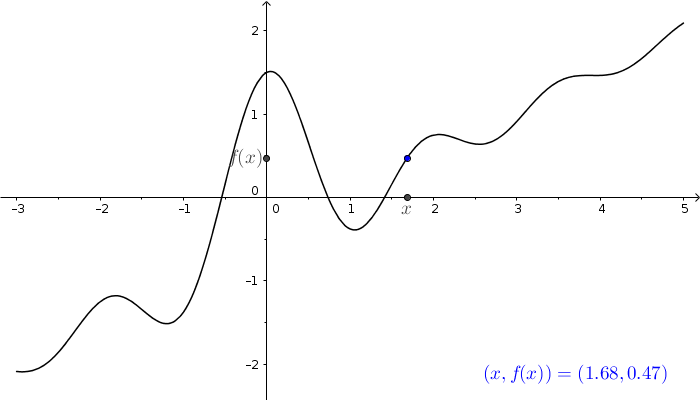
\includegraphics[width=12cm,keepaspectratio=true]{04_Graf_falls.png}
\end{center}


\index{fall!jafnstætt}\index{fall!oddstætt}

\subsection{Skilgreining: Jafnstætt og oddstætt}
\label{kafli01:skilgreining-jafnstaett-og-oddstaett}\label{kafli01:index-10}
Við segjum að fall \(f\) sé \textit{jafnstætt} ef
\begin{equation*}
\begin{split}f(x) = f(-x)\end{split}
\end{equation*}
fyrir öll \(x\) í skilgreiningarmengi \(f\).

Við segjum að fall \(f\) sé \textit{oddstætt} ef
\begin{equation*}
\begin{split}f(x) = -f(-x)\end{split}
\end{equation*}
fyrir öll \(x\) í skilgreiningarmengi \(f\).

\begin{center}
  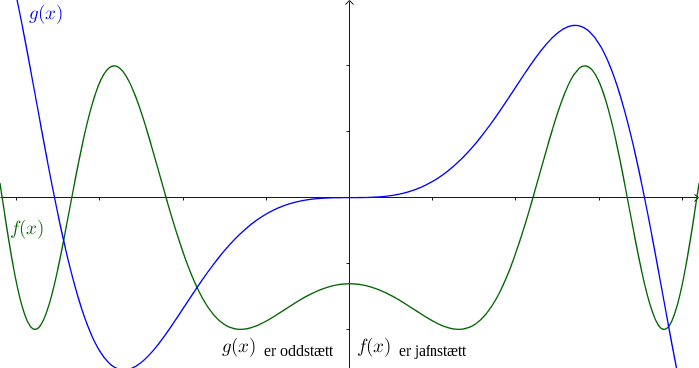
\includegraphics[width=10cm]{04_JafnstaettOddstaett.png}
\end{center}

\chapter{Markgildi og samfelldni}
\label{kafli02:markgildi-og-samfelldni}\label{kafli02::doc}
\begin{notice}{note}{Athugasemd:}
\textbf{Nauðsynleg undirstaða}
\begin{itemize}
\item {} 
Jafna línu, P.2

\item {} 
Jafna hrings, P.3

\item {} 
Hliðrun og skölun grafs, P.3

\item {} 
(Stranglega) minnkandi og (stranglega) vaxandi föll, 2.8

\item {} 
Jafnstæð og oddstæð föll, P.4

\item {} 
Margliður; deiling, þáttun og rætur, P.6

\item {} 
Tölugildisfallið, P.1

\item {} 
Þríhyrningsójafnan, P.1

\item {} 
Formerkjafallið, \(sgn(x)\), P.5

\end{itemize}
\end{notice}

\begin{notice}{warning}{Aðvörun:}
Þessi kafli fjallar um tvö afskaplega mikilvæg og nátengd hugtök,
markgildi og samfelldni. Það er nauðsynlegt fyrir nemendur að ná
góðum tökum á þeim því mörg hugtök í stærðfræði og hagnýtingum á stærðfræði
sem verða á vegi ykkar í framtíðinni byggja á þessum hugtökum.
\end{notice}

\emph{I'd take the awe of understanding over the awe of ignorance any day.}

- Douglas Adams, The Salmon of Doubt


\bigskip\hrule{}\bigskip



\section{Markgildi}
\label{kafli02:markgildi}\label{kafli02:id1}
\index{markgildi}

\subsection{Óformleg skilgreining á markgildi}
\label{kafli02:index-0}\label{kafli02:oformleg-skilgreining-a-markgildi}
Segjum að fall \(f(x)\) \emph{stefni á tölu} \(L\) \emph{þegar} \(x\)
\emph{stefnir á} \(a\), og ritum \(\lim_{x\rightarrow a} f(x)=L\), ef
við getum tryggt að \(f(x)\) sé eins nálægt \(L\) og við
viljum bara með því að velja \(x\) nógu nálægt \(a\).


\subsection{Skilgreining: Markgildi}
\label{kafli02:skilgreining-markgildi}
Gerum ráð fyrir að fall \(f\) sé skilgreint á opnu bili umhverfis
punktinn \(a\), nema hvað hugsanlega er \(f(a)\) ekki
skilgreint. Við segjum að \(f(x)\) \emph{stefni á tölu} \(L\) \emph{þegar}
\(x\) \emph{stefnir á} \(a\), og ritum
\(\lim_{x\rightarrow a} f(x)=L\), ef eftirfarandi skilyrði er
uppfyllt:

Fyrir sérhverja tölu \(\epsilon>0\) er til tala \(\delta>0\)
þannig að um öll \(x\) sem eru þannig að
\begin{equation*}
\begin{split}0 < |x-a| < \delta,\quad \text{ þá gildir } \quad |f(x)-L| <\epsilon.\end{split}
\end{equation*}
Við segjum að talan \(L\) sé \textit{markgildi} \(f(x)\) þegar
\(x\) stefnir á \(a\).


\begin{center}
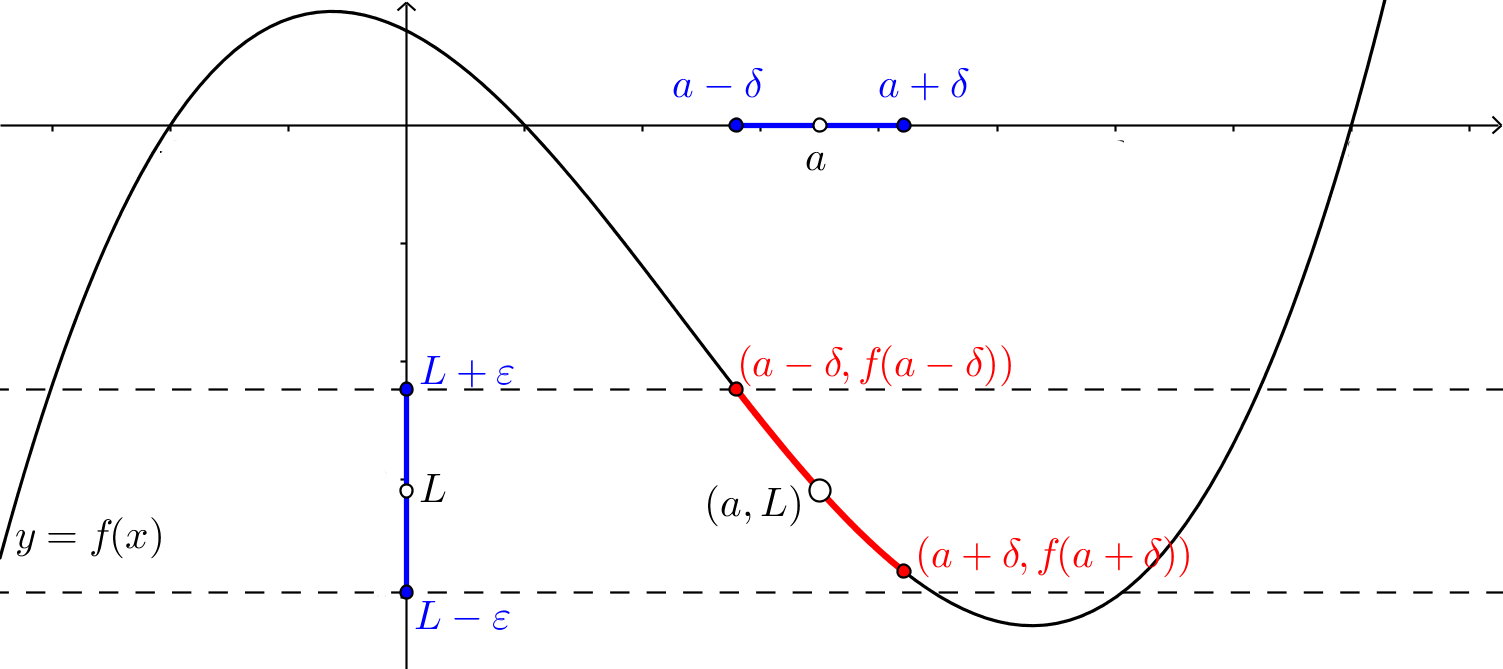
\includegraphics[width=12cm,keepaspectratio=true]{01_markgildi.png}
\end{center}


\begin{notice}{note}{Athugasemd:}
Þegar athugað er hvort markgildið \(\lim_{x\rightarrow a} f(x)\) er
til, og þá hvert gildi þess er, þá skiptir ekki máli hvort \(f(a)\) er
skilgreint eða ekki.
\end{notice}


\subsection{Dæmi}
\label{kafli02:daemi}\label{kafli02:daemi2-1}\begin{enumerate}
\item {} 
\(\lim_{x \to a} c = c\), \(c\) fasti

\item {} 
\(\lim_{x \to a} x = a\)

\item {} 
\(\lim_{x \to a} |x| = |a|\)

\end{enumerate}

Hér er fallið sem um ræðir \(f(x) = x\) og \(L=a\).
Látum \(\epsilon>0\) vera gefið. Við viljum finna
\(\delta >0\) þannig að \(|x-a|<\delta\) hafi í för
með sér \(|f(x)-a| < \epsilon\). Þar sem \(f(x)=x\) þá er seinni
ójafnan jafngild \(|x-a|<\epsilon\). Þetta er sama ójafnan og
\(\delta\) þarf að uppfylla þannig að okkur nægir að velja
\(\delta = \epsilon\). Þá hefur
\begin{equation*}
\begin{split}|x-a| < \delta\end{split}
\end{equation*}
í för með sér að
\begin{equation*}
\begin{split}|f(x) -a| < \epsilon.\end{split}
\end{equation*}
\textbf{Ábendingar fyrir sannanir á liðum 1 og 3}

Til að sanna þetta þá er best að teikna mynd til að átta sig á því hvernig
föllin haga sér. Svo má velja
\begin{enumerate}
\item {} 
\(\delta\) sem hvað sem er.

\end{enumerate}
\begin{enumerate}
\setcounter{enumi}{2}
\item {} 
\(\delta=\epsilon\).

\end{enumerate}


\bigskip\hrule{}\bigskip



\section{Markgildi frá hægri og vinstri}
\label{kafli02:markgildi-fra-haegri-og-vinstri}
\index{markgildi!frá hægri}

\subsection{Óformleg skilgreining}
\label{kafli02:oformleg-skilgreining}\label{kafli02:index-1}
Gerum ráð fyrir að fall \(f\) sé skilgreint á opnu bili
\((a,b)\). Segjum að \(f(x)\) \emph{stefni á tölu} \(L\) \emph{þegar}
\(x\) \emph{stefnir á} \(a\) \emph{frá hægri}, og ritum
\(\lim_{x\rightarrow a^+} f(x)=L\), ef við getum tryggt að
\(f(x)\) sé eins nálægt \(L\) og við viljum bara með því að
velja \(x>a\) nógu nálægt \(a\).


\subsection{Skilgreining: Markgildi frá hægri}
\label{kafli02:skilgreining-markgildi-fra-haegri}
Gerum ráð fyrir að fall \(f\) sé skilgreint á opnu bili
\((a,b)\). Við segjum að \(f(x)\) \emph{stefni á tölu} \(L\)
\emph{þegar} \(x\) \emph{stefnir á} \(a\) \emph{frá hægri}, og ritum
\(\lim_{x\rightarrow a^+} f(x)=L\), ef eftirfarandi skilyrði er
uppfyllt.

Fyrir sérhverja tölu \(\epsilon>0\) er til tala \(\delta>0\)
þannig að um öll \(x\) sem eru þannig að
\begin{equation*}
\begin{split}a<x<a+\delta,\quad \text{ þá er } \quad |f(x)-L| <\epsilon.\end{split}
\end{equation*}

\begin{center}
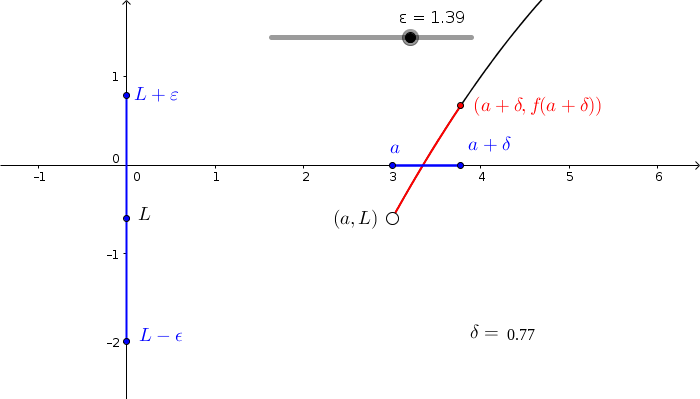
\includegraphics[width=12cm,keepaspectratio=true]{02_markfrahaegri.png}
\end{center}


\index{markgildi!frá vinstri}

\subsection{Óformleg skilgreining}
\label{kafli02:id2}\label{kafli02:index-2}
Gerum ráð fyrir að fall \(f\) sé skilgreint á opnu bili
\((b,a)\). Segjum að \(f(x)\) \emph{stefni á tölu} \(L\) þegar
\(x\) \emph{stefnir á} \(a\) \emph{frá vinstri}, og ritum
\(\lim_{x\rightarrow a^-} f(x)=L\), ef við getum tryggt að
\(f(x)\) sé eins nálægt \(L\) og við viljum bara með því að
velja \(x<a\) nógu nálægt \(a\).


\subsection{Skilgreining: Markgildi frá vinstri}
\label{kafli02:skilgreining-markgildi-fra-vinstri}
Gerum ráð fyrir að fall \(f\) sé skilgreint á opnu bili
\((b,a)\). Við segjum að \(f(x)\) \emph{stefni á tölu} \(L\)
\emph{þegar} \(x\) \emph{stefnir á} \(a\) \emph{frá vinstri}, og ritum
\(\lim_{x\rightarrow a^-} f(x)=L\), ef eftirfarandi skilyrði er
uppfyllt.

Fyrir sérhverja tölu \(\epsilon>0\) er til tala \(\delta>0\)
þannig að um öll \(x\) sem eru þannig að
\begin{equation*}
\begin{split}a-\delta<x<a,\quad \text{ þá er } \quad |f(x)-L| <\epsilon.\end{split}
\end{equation*}

\begin{center}
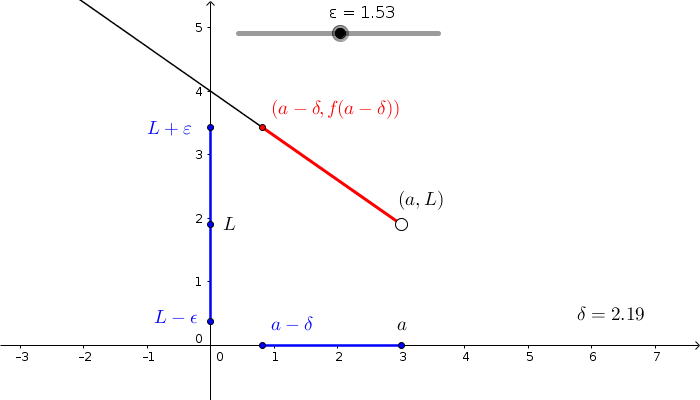
\includegraphics[width=12cm,keepaspectratio=true]{03_markfravinstri.png}
\end{center}



\subsection{Setning}
\label{kafli02:setning-hv-markgildi}\label{kafli02:setning}
Gerum ráð fyrir að fall \(f\) sé skilgreint á opnu bili umhverfis
punktinn \(a\), nema hvað hugsanlega er \(f(a)\) ekki
skilgreint. Þá er
\begin{equation*}
\begin{split}\lim_{x\rightarrow a} f(x)=L\end{split}
\end{equation*}
ef og aðeins ef
\begin{equation*}
\begin{split}\lim_{x\rightarrow a^-} f(x)=L=\lim_{x\rightarrow a^+} f(x).\end{split}
\end{equation*}

\subsection{Dæmi: Tölugildisfallið}
\label{kafli02:daemi-tolugildisfalli}
\textit{Tölugildisfallið} \(|x|\) er skilgreint sem \(x\)
ef \(x\geq 0\) en \(-x\) ef \(x<0\). Um tölugildisfallið gildir
\begin{enumerate}
\item {} \begin{equation*}
\begin{split}\lim_{x\to 0^+} \frac x{|x|} = 1\end{split}
\end{equation*}
\item {} \begin{equation*}
\begin{split}\lim_{x\to 0^-} \frac x{|x|} = -1\end{split}
\end{equation*}
\item {} \begin{equation*}
\begin{split}\lim_{x\to 0} \frac x{|x|} \quad \text{er ekki til}\end{split}
\end{equation*}
\end{enumerate}

\begin{center}
  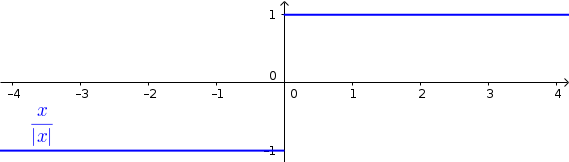
\includegraphics[width=10cm]{02_daemi.png}          
    \end{center}  
\begin{enumerate}
\item {} 
Hér skoðum við eingöngu \(x>0\) og þá gildir að
\(\frac x{|x|} = \frac xx = 1\). Þar sem
\(\lim_{x \to 0} 1 = 1\) samkvæmt {\hyperref[kafli02:daemi2\string-1]{\sphinxcrossref{\DUrole{std,std-ref}{Dæmi 2.1.3}}}}
þá gildir einni að \(\lim_{x \to 0^+} 1 = 1\) samkvæmt
{\hyperref[kafli02:setning\string-hv\string-markgildi]{\sphinxcrossref{\DUrole{std,std-ref}{setningunni}}}}
hér á undan. Þannig að
\begin{equation*}
\begin{split}\lim_{x \to 0^+} \frac x{|x|} =
\lim_{x \to 0^+} 1 = 1\end{split}
\end{equation*}
\item {} 
Eins og liður 1 nema ef \(x<0\) þá er
\(\frac x{|x|} = \frac x{-x} = -1\)

\item {} 
Af liðum 1 og 2 sést að hægri og vinstri markgildin eru ekki þau sömu þannig
að samkvæmt {\hyperref[kafli02:setning\string-hv\string-markgildi]{\sphinxcrossref{\DUrole{std,std-ref}{setningunni}}}} hér á undan þá er
markgildið ekki til.

\end{enumerate}


\bigskip\hrule{}\bigskip



\section{Reiknireglur fyrir markgildi}
\label{kafli02:reiknireglur-fyrir-markgildi}

\subsection{Setning}
\label{kafli02:id3}\label{kafli02:setning-markgildi}
Gerum ráð fyrir að \(\lim_{x\rightarrow a}f(x)=L\) og að
\(\lim_{x\rightarrow a}g(x)=M\). Þá gildir
\begin{enumerate}
\item {} 
\(\lim_{x\rightarrow a}\Big(f(x)+g(x)\Big)=L+M\).

\item {} 
\(\lim_{x\rightarrow a}\Big(f(x)-g(x)\Big)=L-M\).

\item {} 
\(\lim_{x\rightarrow a}f(x)g(x)=LM\).

\item {} 
\(\lim_{x\rightarrow a}kf(x)=kL\), þar sem \(k\) fasti.

\item {} 
\(\lim_{x\rightarrow a}f(x)/g(x)=L/M\), að því gefnu að
\(M\neq 0\).

\item {} 
Gerum ráð fyrir að \(m\) og \(n\) séu heiltölur þannig að
\(f(x)^{m/n}\) sé skilgreint fyrir öll \(x\) á bili
\((b,c)\) umhverfis \(a\) (en ekki endilega fyrir
\(x=a\)) og að \(L^{m/n}\) sé skilgreint. Þá er
\(\lim_{x\rightarrow a}f(x)^{m/n}=L^{m/n}\).

\item {} 
Ef til er bil \((b,c)\) sem inniheldur \(a\) þannig að
\(f(x)\leq g(x)\) fyrir öll \(x\in (b,c)\), nema kannski
\(x=a\), þá er
\(\lim_{x\rightarrow a}f(x)=L\leq M=\lim_{x\rightarrow a}g(x)\).

\end{enumerate}

\begin{notice}{warning}{Aðvörun:}
Liður (i) í setningunni á undan segir að ef markgildin
\(\lim_{x\to a} f(x)\) og \(\lim_{x\to a} g(x)\) eru til þá sé
markgildið \(\lim_{x\to a} (f(x)+g(x))\) einnig til.

En hún segir \textbf{ekki} að ef \(f\) og \(g\) eru föll þannig að
markgildið \(\lim_{x\to a} (f(x)+g(x))\) er til, að þá séu
markgildin \(\lim_{x\to a} f(x)\) og \(\lim_{x\to a} g(x)\)
einnig til.
\end{notice}

\textbf{Sönnun á lið 1}

Við viljum sýna að fyrir \(\epsilon>0\) þá sé til \(\delta>0\)
þannig að ef \(|x-a|<\delta\) þá sé \(|f(x)+g(x) - (L+M)|<\epsilon\).
Látum nú \(\epsilon>0\) vera gefið, þá fæst af
\(\lim_{x\to a} f(x) = L\) að til er \(\delta_1>0\) þannig að
\begin{equation*}
\begin{split}|f(x)-L| < \frac \epsilon 2\end{split}
\end{equation*}
ef \(|x-a|<\delta_1\). Eins fæst af \(\lim_{x \to a} g(x)=M\)
að til er \(\delta_2\) þannig að
\begin{equation*}
\begin{split}|g(x)-M| < \frac \epsilon 2\end{split}
\end{equation*}
ef \(|x-a|<\delta_2\).

Ef við setjum \(\delta = \min\{\delta_1,\delta_2\}\) þá þýðir það að
öll \(x\) sem uppfylla \(|x-a|<\delta\) uppfylla einnig
\(|x-a|<\delta_1\) og \(|x-a|<\delta_2\). Þá gefur þríhyrningsójafnan
okkur að fyrir slíkt \(x\) þá er
\begin{equation*}
\begin{split}|f(x)+g(x) - (L+M)| = |f(x)-L + g(x)-M| \\
< |f(x)-L| + |g(x)-M| < \frac \epsilon 2 + \frac \epsilon 2 = \epsilon,\end{split}
\end{equation*}
sem er það sem við vildum sýna.

\index{klemmureglan}

\subsection{Setning: Klemmureglan}
\label{kafli02:setning-klemmureglan}\label{kafli02:index-3}
Gerum ráð fyrir að \(f(x)\leq
g(x)\leq h(x)\) fyrir öll \(x\) á bili \((b, c)\) sem inniheldur
\(a\), nema kannski \(x=a\). Gerum enn fremur ráð fyrir að
\begin{equation*}
\begin{split}\lim_{x\rightarrow a}f(x)=\lim_{x\rightarrow a}h(x)=L.\end{split}
\end{equation*}
Þá er \(\lim_{x\rightarrow a}g(x)=L\).

\noindent{\hspace*{\fill}\sphinxincludegraphics[width=0.800\linewidth]{{04_03_klemmuregla}.png}\hspace*{\fill}}

\textbf{Sönnun}

Látum \(\epsilon>0\) vera gefið. Við viljum sýna að þá sé til \(\delta>0\) þannig
að \(|g(x)-L|<\epsilon\) fyrir öll \(x\) sem uppfylla \(|x-a|<\delta\).

Þetta má líka skrifa svona:
Við viljum sýna að þá sé til \(\delta>0\) þannig
að \(L-\epsilon<g(x)<L+\epsilon\) fyrir öll \(x\) sem uppfylla \(a-\delta < x<a+\delta\).

Við vitum nú að þar sem \(\lim_{x\to a} f(x) = L\) þá er til \(\delta_1\)
þannig að \(L-\epsilon<f(x)<L+\epsilon\) fyrir öll \(x\) sem uppfylla \(a-\delta_1 < x<a+\delta_1\).

Eins þá fæst af \(\lim_{x\to a} h(x) = L\) að til er \(\delta_2\)
þannig að \(L-\epsilon<g(x)<L+\epsilon\) fyrir öll \(x\) sem uppfylla \(a-\delta_2 < x<a+\delta_2\).

Setjum nú \(\delta = \min\{\delta_1,\delta_2\}\) og athugum að það þýðir að fyrir sérhvert \(x\) sem
uppfyllir \(a-\delta < x < a+\delta\) uppfyllir einnig \(a-\delta_1 < x<a+\delta_1\)
og \(a-\delta_2 < x<a+\delta_2\). Þá gefur \(f(x)\leq g(x)\leq h(x)\) að
\begin{equation*}
\begin{split}L-\epsilon<f(x) \leq g(x) \leq h(x) < L+\epsilon.\end{split}
\end{equation*}
Þar með er \(L-\epsilon < g(x) < L+\epsilon\) og þá höfum við sýnt að
\(\lim_{x\to a} g(x) = L\).


\subsection{Dæmi: Markgildi með sínus}
\label{kafli02:daemi-markgildi-me-sinus}\begin{enumerate}
\item {} \begin{equation*}
\begin{split}\lim_{x\to 0} \sin\left(\frac 1x\right) \quad \text{er ekki til}\end{split}
\end{equation*}
\item {} \begin{equation*}
\begin{split}\lim_{x\to 0} x\sin\left(\frac 1x\right) = 0\end{split}
\end{equation*}
\item {} \begin{equation*}
\begin{split}\lim_{x \to 0} \frac{\sin(x)}{x} = 1\end{split}
\end{equation*}
\end{enumerate}

Sönnum þetta með mótsögn. Gerum ráð fyrir að til sé markgildi \(L\) þannig að fyrir
sérhvert \(\epsilon >0\) er til \(\delta>0\) þannig að
\(|x-0|<\delta\) hefur í för með sér að \(|\sin(1/x) - L|<\epsilon\). Til þess
að þetta leiði til mótsagnar þurfum við að finna \(\epsilon>0\) sem er þannig að
sama hversu lítið \(\delta>0\) er valið þá er alltaf til \(x\) þannig að
\(|x-0|<\delta\) og
\begin{equation*}
\begin{split}\left|\sin\left(\frac 1x \right)-L\right| \geq \epsilon.\end{split}
\end{equation*}
Veljum \(\epsilon = 0,5\). Ástæðan fyrir þessu vali er sú að þar sem
\(\sin(1/x)\) sveiflast á milli \(-1\) og \(1\) þá er nóg að
velja tölu sem er þannig að fallið sveiflist út
fyrir bilið \([L-\epsilon,L+\epsilon]\). Í þessu tilviki þýðir það að
\(\epsilon\) þarf að vera minna en 1.

Ef markgildið er til þá er ætti að vera til \(\delta>0\) þannig að
\(|\sin(1/x)-L|< 0.5\) fyrir \(x\) sem uppfylla \(|x-0|<\delta\).
Byrjum á að skoða tilvikið \(L\leq 0\).
Finnum nógu stóra náttúrlega tölu \(k\)
þannig að \(\frac 1{2\pi k + \pi/2} < \delta\).
Ef við setjum \(x=\frac 1{2\pi k + \pi/2}\)
þá fæst að \(|x-0|<\delta\) en
\begin{equation*}
\begin{split}\left|\sin\left(\frac 1x \right) - L\right| =
|\sin(2\pi k +\pi/2) - L|  = |1-L| > 0,5\end{split}
\end{equation*}
Tilvikið þegar \(L>0\) er eins nema þá veljum við \(x=\frac 1{2\pi k - \pi/2}\)
sem þýðir að \(\sin(x) = -1\).


\begin{center}
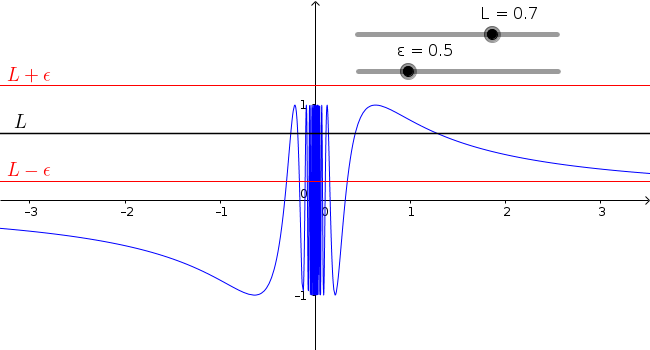
\includegraphics[width=12cm,keepaspectratio=true]{03_daemi-sin.png}
\end{center}



\section{Markgildi þegar x stefnir á óendanlegt}
\label{kafli02:markgildi-egar-x-stefnir-a-oendanlegt}
\noindent{\hspace*{\fill}\sphinxincludegraphics[width=0.500\linewidth]{{06_liminf}.png}\hspace*{\fill}}

\index{markgildi!þegar x stefnir á óendalegt}

\subsection{Óformleg skilgreining}
\label{kafli02:id4}\label{kafli02:index-4}
Gerum ráð fyrir að fall \(f\) sé skilgreint á bili
\((a, \infty)\). Segjum að \(f(x)\) \emph{stefni á tölu} \(L\)
\emph{þegar} \(x\) \emph{stefnir á} \(\infty\), og ritum
\(\lim_{x\rightarrow \infty} f(x)=L\), ef við getum tryggt að
\(f(x)\) sé eins nálægt \(L\) og við viljum bara með því að
velja \(x\) nógu stórt.


\subsection{Skilgreining: Markgildi þegar \protect\(x \to \infty\protect\)}
\label{kafli02:skilgreining-markgildi-egar}
Gerum ráð fyrir að fall \(f\) sé skilgreint á bili
\((a,\infty)\). Við segjum að \(f(x)\) \emph{stefni á tölu} \(L\)
\emph{þegar} \(x\) \emph{stefnir á} \(\infty\), og ritum
\(\lim_{x\rightarrow \infty} f(x)=L\), ef eftirfarandi skilyrði er
uppfyllt:

Fyrir sérhverja tölu \(\epsilon>0\) er til tala \(R\)
þannig að um öll \(x>R\) gildir að
\begin{equation*}
\begin{split}|f(x)-L|<\epsilon.\end{split}
\end{equation*}

\subsection{Óformleg skilgreining}
\label{kafli02:id5}
Fyrir \(-\infty\) er þetta gert með sama sniði.

Gerum ráð fyrir að fall \(f\) sé skilgreint á bili
\((-\infty, a)\). Segjum að \(f(x)\) \emph{stefni á tölu} \(L\)
\emph{þegar} \(x\) \emph{stefnir á} \(-\infty\), og ritum
\(\lim_{x\rightarrow -\infty} f(x)=L\), ef við getum tryggt að
\(f(x)\) sé eins nálægt \(L\) og við viljum bara með því að
velja \(x\) sem nógu stóra neikvæða tölu.


\subsection{Skilgreining: Markgildi þegar \protect\(x \to -\infty\protect\)}
\label{kafli02:id6}
Gerum ráð fyrir að fall \(f\) sé skilgreint á bili
\((-\infty,a)\). Við segjum að \(f(x)\) \emph{stefni á tölu}
\(L\) \emph{þegar} \(x\) \emph{stefnir á} \(-\infty\), og ritum
\(\lim_{x\rightarrow -\infty} f(x)=L\), ef eftirfarandi skilyrði er
uppfyllt:

Fyrir sérhverja tölu \(\epsilon>0\) er til tala \(R\)
þannig að um öll \(x<R\) gildir að
\begin{equation*}
\begin{split}|f(x)-L|<\epsilon.\end{split}
\end{equation*}

\bigskip\hrule{}\bigskip



\section{Óendanlegt sem markgildi}
\label{kafli02:oendanlegt-sem-markgildi}
\index{markgildi!óendanlegt sem markgildi}

\subsection{Óformleg skilgreining}
\label{kafli02:index-5}\label{kafli02:id7}
Gerum ráð fyrir að fall \(f\) sé skilgreint á opnu bili umhverfis
punktinn \(a\), nema hvað hugsanlega er \(f(a)\) ekki
skilgreint. Segjum að \(f(x)\) \emph{stefni á} \(\infty\) \emph{þegar}
\(x\) \emph{stefnir á} \(a\), og ritum
\(\lim_{x\rightarrow a} f(x)=\infty\), ef við getum tryggt að
\(f(x)\) sé \emph{hversu stórt sem við viljum} bara með því að velja
\(x\) \emph{nógu nálægt} \(a\).


\subsection{Skilgreining: Markgildið \protect\(\infty\protect\)}
\label{kafli02:id8}
Gerum ráð fyrir að fall \(f\) sé skilgreint á opnu bili umhverfis
punktinn \(a\), nema hvað hugsanlega er \(f(a)\) ekki
skilgreint. Við segjum að \(f(x)\) \emph{stefni á} \(\infty\) \emph{þegar}
\(x\) \emph{stefnir á} \(a\), og ritum
\(\lim_{x\rightarrow a} f(x)=\infty\), ef eftirfarandi skilyrði er
uppfyllt.

Fyrir sérhverja tölu \(B\) er til tala \(\delta>0\) þannig
að um öll \(x\) sem eru þannig að
\begin{equation*}
\begin{split}0 < |x-a| <\delta \quad  \text{ gildir að } \quad f(x) > B.\end{split}
\end{equation*}
\begin{notice}{warning}{Aðvörun:}
Athugið að \(\infty\) er \textbf{ekki} tala. Þó að
\(\lim_{x\rightarrow a} f(x)=\infty\) þá er samt sagt að markgildið
\(\lim_{x\rightarrow a} f(x)\) sé ekki til.
\end{notice}


\subsection{Óformleg skilgreining}
\label{kafli02:id9}
Gerum ráð fyrir að fall \(f\) sé skilgreint á opnu bili umhverfis
punktinn \(a\), nema hvað hugsanlega er \(f(a)\) ekki
skilgreint. Segjum að \(f(x)\) \emph{stefni á} \(-\infty\) \emph{þegar}
\(x\) \emph{stefnir á} \(a\), og ritum
\(\lim_{x\rightarrow a} f(x)=-\infty\), ef við getum tryggt að
\(f(x)\) sé hversu lítið sem við viljum bara með því að velja
\(x\) nógu nálægt \(a\).


\subsection{Skilgreining: Markgildið \protect\(-\infty\protect\)}
\label{kafli02:id10}
Gerum ráð fyrir að fall \(f\) sé skilgreint á opnu bili umhverfis
punktinn \(a\), nema hvað hugsanlega er \(f(a)\) ekki
skilgreint. Við segjum að \(f(x)\) \emph{stefni á} \(-\infty\)
\emph{þegar} \(x\) \emph{stefnir á} \(a\), og ritum
\(\lim_{x\rightarrow a} f(x)=-\infty\), ef eftirfarandi skilyrði er
uppfyllt.

Fyrir sérhverja tölu \(B\) er til tala \(\delta>0\) þannig
að um öll \(x\) sem eru þannig að
\begin{equation*}
\begin{split}0 < |x-a| < \delta \quad \text{ gildir að } \quad f(x)<B.\end{split}
\end{equation*}
\begin{notice}{warning}{Aðvörun:}
Athugið að \(-\infty\) er \textbf{ekki} tala. Þó að
\(\lim_{x\rightarrow a} f(x)=-\infty\) þá er samt sagt að markgildið
\(\lim_{x\rightarrow a} f(x)\) sé ekki til.
\end{notice}

\index{samfelldni}\index{samfelldni!í punkti}

\bigskip\hrule{}\bigskip



\section{Samfelldni}
\label{kafli02:samfelldni}\label{kafli02:id11}
Hér skilgreinum við og skoðum seinna grundvallarhugtakið í þessum kafla, sem er \textit{samfelldni}.

\index{innri punktur}

\subsection{Skilgreining: Innri punktur}
\label{kafli02:skilgreining-innri-punktur}\label{kafli02:index-7}
Látum \(A\subseteq {{\mathbb  R}}\) og \(x\in A\). Við segjum að
\(x\) sé \textit{innri punktur} \(A\) ef \(A\) inniheldur opið bil
umhverfis \(x\), það er að segja til er tala \(\delta>0\) þannig
að \((x-\delta, x+\delta)\subseteq
A\).

Ef \(x\) er ekki innri punktur \(A\) og \(x\in A\) þá segjum
við að \(x\) sé \textit{jaðarpunktur} \(A\).

\index{samfelldni!í punkti}

\subsection{Skilgreining: Samfelldni í punkti}
\label{kafli02:skilgreining-samfelldni-i-punkti}\label{kafli02:index-8}
Látum \(f\) vera fall og \(c\) innri punkt skilgreiningarsvæðis
\(f\). Sagt er að \(f\) sé \emph{samfellt í punktinum} \(c\) ef
\begin{equation*}
\begin{split}\lim_{x\rightarrow c}f(x)=f(c).\end{split}
\end{equation*}

\subsection{Setning}
\label{kafli02:id12}
Látum \(f\) og \(g\) vera föll. Gerum ráð fyrir að \(c\) sé
innri punktur skilgreiningarsvæðis beggja fallanna og að bæði föllin séu
samfelld í punktinum \(c\). Þá eru eftirfarandi föll samfelld í
\(c\):
\begin{enumerate}
\item {} 
\(f+g\)

\item {} 
\(f-g\)

\item {} 
\(fg\)

\item {} 
\(kf\), þar sem \(k\) er fasti

\item {} 
\(f/g\), ef \(g(c)\neq 0\)

\item {} 
\(\Big(f(x)\Big)^{1/n}\), að því gefnu að \(f(c)>0\) ef
\(n\) er slétt tala og \(f(c)\neq 0\) ef \(n<0\).

\end{enumerate}

Þessi setning er bein afleiðing af {\hyperref[kafli02:setning\string-markgildi]{\sphinxcrossref{\DUrole{std,std-ref}{Setningu 2.3.1}}}}.


\subsection{Setning: Samskeyting samfelldra falla}
\label{kafli02:setning-samskeyting-samfelldra-falla}
Látum \(g\) vera fall sem er skilgreint á opnu bili umhverfis
\(c\) og samfellt í \(c\) og látum \(f\) vera fall sem er
skilgreint á opnu bili umhverfis \(g(c)\) og samfellt í
\(g(c)\). Þá er fallið \(f\circ g\) skilgreint á opnu bili
umhverfis \(c\) og er samfellt í \(c\).

\begin{notice}{note}{Athugasemd:}
Ef fall er skilgreint með formúlu og skilgreingamengið er ekki tilgreint
sérstaklega, þá er venjan að líta alla þá punkta þar sem formúlan gildir
sem skilgreingarmengi fallsins
\end{notice}

\index{samfelldni}\index{samfellt fall}

\subsection{Skilgreining: Samfellt fall}
\label{kafli02:index-9}\label{kafli02:skilgrsamfellt}\label{kafli02:skilgreining-samfellt-fall}
Við segjum að fall \(f\) sé \textit{samfellt} ef það er samfellt í
sérhverjum punkti skilgreingarmengisins.

Óformlega þýðir þetta að hægt er að teikna graf \(f\) án þess að lyfta pennanum frá blaðinu.


\subsection{Dæmi}
\label{kafli02:id13}
Eftirfarandi föll eru samfelld
\begin{enumerate}
\item {} 
margliður

\item {} 
ræð föll

\item {} 
ræð veldi

\item {} 
hornaföll; \(\sin\), \(\cos\), \(\tan\)

\item {} 
tölugildisfallið \(|x|\)

\end{enumerate}


\subsection{Að búa til samfelld föll}
\label{kafli02:a-bua-til-samfelld-foll}
Með því að nota föllin úr dæminu á undan sem efnivið þá getum við búið
til fjölda samfelldra fall með því að beita aðgerðunum úr Setningu 2.6.4
og Setningu 2.6.3.

\index{samfelldni!frá hægri/vinstri}

\subsection{Dæmi}
\label{kafli02:id14}\label{kafli02:index-10}
Fallið \(\cos(3x+5)\) er samfellt. Margliðan \(g(x) =3x+5\) og
\(f(x) = \cos(x)\) eru samfelld föll og þá er samskeytingin
\(f\circ g(x) = \cos(3x+5)\) einnig samfellt fall.


\bigskip\hrule{}\bigskip



\section{Hægri/vinstri samfelldni}
\label{kafli02:haegri-vinstri-samfelldni}
Rifjum upp skilgreininguna á samfelldni.


\subsection{Skilgreining}
\label{kafli02:skilgreining}
Látum \(f\) vera fall og \(c\) innri punkt skilgreiningarsvæðis
\(f\). Sagt er að \(f\) sé \emph{samfellt í punktinum} \(c\) ef
\begin{equation*}
\begin{split}\lim_{x\rightarrow c}f(x)=f(c).\end{split}
\end{equation*}

\subsection{Athugasemd}
\label{kafli02:athugasemd}
Þessi skilgreining virkar aðeins fyrir innri punkta
skilgreiningarsvæðisins. Þannig að ef ætlunin er að rannsaka samfelldni
í jaðarpunktum þá gengur þessi skilgreining ekki. Hins vegar getum við
útvíkkað skilgreininguna á samfelldni fyrir hægri og vinstri endapunkta
bila með því að einskorða okkur við markgildi frá vinstri og hægri.


\subsection{Skilgreining: Hægri/vinstri samfelldni}
\label{kafli02:skilgreining-haegri-vinstri-samfelldni}\begin{enumerate}
\item {} 
Fall \(f\) er \emph{samfellt frá hægri í punkti} \(c\) ef
\(\lim_{x\rightarrow c^+}f(x)=f(c)\).

Hér er gert ráð fyrir að fallið \(f\) sé amk. skilgreint á
bili \([c, a)\).

\item {} 
Fall \(f\) er \emph{samfellt frá vinstri í punkti} \(c\) ef
\(\lim_{x\rightarrow c^-}f(x)=f(c)\).

Hér er gert ráð fyrir að fallið \(f\) sé amk. skilgreint á
bili \((a, c]\).

\end{enumerate}

Uppfærum nú skilgreininguna á {\hyperref[kafli02:skilgrsamfellt]{\sphinxcrossref{\DUrole{std,std-ref}{samfelldu falli}}}}.

\index{fall!samfellt}

\subsection{Uppfærð skilgreining: Samfellt fall}
\label{kafli02:index-11}\label{kafli02:uppfaer-skilgreining-samfellt-fall}
Gerum ráð fyrir að \(f\) sé fall sem er skilgreint á mengi
\(A\), þar sem \(A\) er sammengi endanlega margra bila. Við
segjum að fallið \(f\) sé \emph{samfellt} ef það er samfellt í öllum
innri punktum skilgreingarmengisins og ef það er samfellt frá
hægri/vinstri í jaðarpunktum skilgreingarmengisins, eftir því sem við á.

\begin{notice}{note}{Athugasemd:}
Ef fall er samfellt á opnu bili \((a,b)\), og ef \(a<c<d<b\), þá
er fallið einnig samfellt á bilinu \([c,d]\).
\end{notice}


\bigskip\hrule{}\bigskip



\section{Eiginleikar samfelldra falla}
\label{kafli02:eiginleikar-samfelldra-falla}
\index{há- og lággildislögmálið}

\subsection{Setning – Há- og lággildislögmálið}
\label{kafli02:ha-og-laggildislogmali}\label{kafli02:setning-ha-og-laggildislogmali}\label{kafli02:index-12}
Látum \(f\) vera samfellt fall skilgreint á \textbf{lokuðu takmörkuðu bili}
\([a,b]\). Þá eru til tölur \(x_1\) og \(x_2\) í
\([a,b]\) þannig að fyrir allar tölur \(x\) í \([a,b]\) er
\begin{equation*}
\begin{split}f(x_1)\leq f(x)\leq f(x_2).\end{split}
\end{equation*}
Þetta þýðir að samfellt fall \(f\) á lokuðu og takmörkuðu bili
\([a,b]\) tekur bæði hæsta og lægsta gildi á bilinu. Hæsta gildið er
þá \(f(x_2)\) og lægsta gildið er \(f(x_1)\).

\begin{notice}{note}{Athugasemd:}
Það er mögulegt að fallið taki há/lággildi sitt í fleiri en einum
punkti.
\end{notice}

\index{milligildissetningin}

\subsection{Setning: Milligildissetningin}
\label{kafli02:index-13}\label{kafli02:setning-milligildissetningin}
Látum \(f\) vera samfellt fall skilgreint á lokuðu takmörkuðu bili
\([a,b]\). Gerum ráð fyrir að \(s\) sé tala sem liggur á milli
\(f(a)\) og \(f(b)\). Þá er til tala \(c\) sem liggur á
milli \(a\) og \(b\) þannig að \(f(c)=s\).


\begin{center}
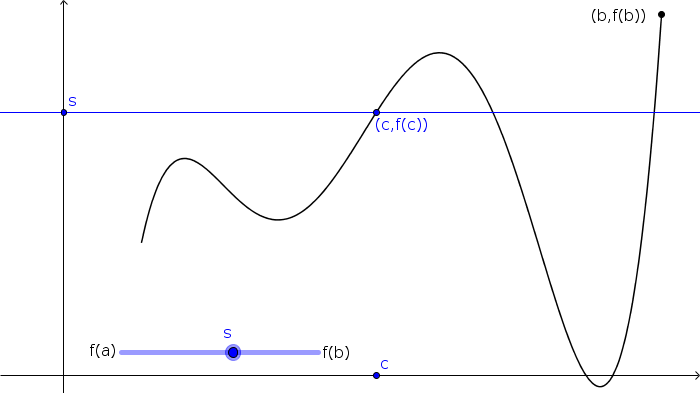
\includegraphics[width=12cm,keepaspectratio=true]{10_milligildissetn.png}
\end{center}


\textbf{Sönnun}

Í setningunni þá gerum við ráð fyrir að \(s\) liggi á milli \(f(a)\) og
\(f(b)\). Til að svona \(s\) sé til þá þarf \(f(a) \neq f(b)\).

Skoðum tilvikið þegar \(f(a) < f(b)\), en þá er \(f(a) < s < f(b)\).
Tilvikið \(f(a)>f(b)\) er nánast eins.

Skilgreinum mengið \(S = \{ x \in [a,b] ; f(x) < s\}\). Þetta mengi er ekki tómt
því \(a\) er í því og það er takmarkað að ofan af \(b\). Samkvæmt
{\hyperref[kafli01:frumsendanumeframark]{\sphinxcrossref{\DUrole{std,std-ref}{Frumsendunni um efra mark}}}} þá er til efra mark \(c \in[a,b]\)
fyrir \(S\). Við viljum sýna að \(f(c)=s\).

Ef \(f(c)>s\) þá segir samfelldni \(f\)
okkur að til sé lítið bil kringum \(c\) þar sem fallið er stærra en \(s\). Sér í lagi er
til tala minni en \(c\) sem er ekki í menginu \(A\). Þetta þýðir að \(c\) er
ekki minnsta efra mark \(A\). Orðum þetta aðeins nákvæmar.

Veljum \(0<\epsilon < f(c)-s\) þá er til \(\delta>0\) þannig að ef \(x\in ]c-\delta,c+\delta[\)
þá er \(|f(c)-f(x)|<\epsilon < f(c) -s\). Þetta hefur í för með sér að \(f(c) - f(x) < f(c) -s\),
það er \(f(x)>s\). Þetta þýðir að öll \(x\in]c-\delta,c[\) eru ``minni'' efri mörk fyrir \(A\)
en \(c\) sem gengur ekki og er því mótsögn.

Ef \(f(c)<s\) þá segir samfelldni \(f\) okkur að til sé lítið bil kringum \(c\)
þar sem fallið er minna en \(s\). Sér í lagi  er til tala stærri en \(c\) sem er í menginu
\(A\). Þetta þýðir að \(c\) er ekki efra mark, því efra mark á að vera stærra eða jafnt
og öll stök í \(A\). Þetta er einnig mótsögn.

Þá er bara eftir möguleikinn \(f(c)=s\), sem nákvæmlega það sem við vildum.

\begin{notice}{note}{Athugasemd:}
Það er möguleiki að það séu fleiri en einn punktur á bilinu þar sem fallið tekur
gildið \(s\). Sönnunin hér á undan finnur þann stærsta.
\end{notice}


\subsection{Fylgisetning}
\label{kafli02:fylgisetning}
Ef \(P(x)=a_nx^n+a_{n-1}x^{n-1}+\cdots+a_1x+a_0\) er margliða af
oddatölu stigi \(n\), þá er til rauntala \(c\) þannig að \(P(c)=0\).

\textbf{Sönnun}

Gerum ráð fyrir að \(a_n>0\). Þá er
\(\lim_{x\to -\infty} P(x) = -\infty\) og
\(\lim_{x\to \infty} P(x) = \infty\). Það þýðir að til eru tölur
\(a\) og \(b\) þannig að \(P(a)<0\) og \(P(b)>0\). Með
því að beita Milligildissetningunni á fallið \(P\) á bilinu
\([a,b]\) og með \(s=0\) þá fæst að til er núllstöð á bilinu
\([a,b]\).

Ef \(a_n < 0\) þá víxlast formerkin á markgildunum hér að ofan en röksemdafærslan er
að öðru leyti eins.


\chapter{Afleiður}
\label{kafli03:afleiur}\label{kafli03::doc}
\begin{notice}{note}{Athugasemd:}
\textbf{Nauðsynleg undirstaða}
\begin{itemize}
\item {} 
{\hyperref[kafli02:markgildi]{\sphinxcrossref{\DUrole{std,std-ref}{Markgildi}}}}

\item {} 
{\hyperref[kafli02:samfelldni]{\sphinxcrossref{\DUrole{std,std-ref}{Samfelldni}}}}

\item {} 
{\hyperref[kafli01:samskeyting]{\sphinxcrossref{\DUrole{std,std-ref}{samskeyting falla}}}}

\item {} 
{\hyperref[kafli01:andhverfa]{\sphinxcrossref{\DUrole{std,std-ref}{andhverfur falla}}}}

\item {} 
hornaföll, P7

\end{itemize}
\end{notice}

\emph{He felt that his whole life was some kind of dream and he sometimes wondered whose it was and whether they were enjoying it.}

-- Douglas Adams, The Hitchhiker's Guide to the Galaxy


\bigskip\hrule{}\bigskip


\index{afleiða}

\section{Skilgreining á afleiðu}
\label{kafli03:skilgreining-a-afleiu}\label{kafli03:index-0}\label{kafli03:afleidur}

\subsection{Skilgreining: Afleiða}
\label{kafli03:skilgreining-afleia}
Látum \(a\) vera innri punkt skilgreiningarsvæðis falls \(f\).
\textit{Afleiða falls} \(f\) \emph{í punkti} \(a\) er skilgreind sem
\begin{equation*}
\begin{split}f'(a)=\lim_{h\rightarrow 0}\frac{f(a+h)-f(a)}{h}.\end{split}
\end{equation*}
Ef markgildið er til þá er sagt að fallið \(f\) sé
\textit{diffranlegt} \emph{í
punktinum} \(a\), en annars er sagt að fallið sé \emph{ekki diffranlegt í
punktinum} \(a\).


\subsection{Dæmi}
\label{kafli03:daemi}
Fallið \(f(x) = x^2\) er diffranlegt í sérhverjum punkti \(a\).
Það sést af því að
\begin{equation*}
\begin{split}\begin{aligned}
\lim_{h\to 0} \frac{f(a+h)-f(a)}{h}
&= \lim_{h\to 0} \frac{(a+h)^2-a^2}{h}\\
&= \lim_{h\to 0} \frac{a^2+2ah+h^2-a^2}{h}\\
&= \lim_{h\to 0} \frac{2ah+h^2}{h}\\
&= \lim_{h\to 0} 2a+h = 2a.\end{aligned}\end{split}
\end{equation*}

\begin{center}
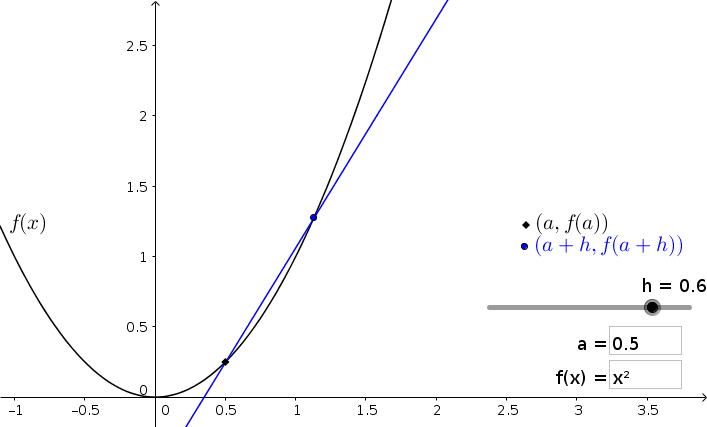
\includegraphics[width=12cm,keepaspectratio=true]{./01_afleida.png}
\end{center}



\subsection{Setning}
\label{kafli03:setning}
Ef fall \(f\) er diffranlegt í punkti \(c\) þá er \(f\)
samfellt í punktinum \(c\).

\textbf{Sönnun}

Skoðum markgildið \(f'(x)=\lim_{h\to 0} \frac{f(c+h)-f(c)}{h}\). Þar
sem \(h\to 0\) þá verður teljarinn einnig að stefna á 0. Það er
\(\lim_{h \to 0} f(c+h)-f(c) = 0\), eða
\(\lim_{h \to 0} f(c+h) = f(c)\). Þetta má einnig rita
\(\lim_{x \to c} f(x) = f(c)\), sem þýðir að fallið \(f\) er
samfellt í \(x=c\).

\begin{notice}{warning}{Aðvörun:}
Fall getur verið samfellt í punkti \(c\) án þess að það sé
diffranlegt í \(c\).
\end{notice}


\subsection{Dæmi}
\label{kafli03:id1}
Fallið \(f(x) = |x|\) er samfellt. En það er ekki diffranlegt í
punktinum \(x=0\). Það sést af því að
\begin{equation*}
\begin{split}\lim_{h\to 0^+} \frac{f(0+h)-f(0)}{h} = \lim_{h\to 0^+} \frac{|h|}{h} = 1\end{split}
\end{equation*}
en
\begin{equation*}
\begin{split}\lim_{h\to 0^-} \frac{f(0+h)-f(0)}{h} = \lim_{h\to 0^-} \frac{|h|}{h} = -1.\end{split}
\end{equation*}
Það er, markgildið \(\lim_{h\to 0} \frac{f(0+h)-f(0)}{h}\) er ekki til.

\index{snertill}\index{sniðill}\index{snertill|see{sniðill}}\index{sniðill|see{snertill}}

\subsection{Snertill}
\label{kafli03:snertill}\label{kafli03:index-1}
Afleiðu falls \(f\) í punktinum \(a\) fæst með því að taka
\textit{sniðil} í gegnum punktana \((a,f(a))\) og \((a+h,f(a+h))\), og
láta svo \(h\) stefna á \(0\).

Þetta gefur hallatölu \textit{snertilsins} við graf fallsins í punktinum
\((a,f(a))\)

Jafna snertils við graf fallsins í punktingum \(a\) er línan
\begin{equation*}
\begin{split}y = f'(a)(x-a) + f(a).\end{split}
\end{equation*}

\begin{center}
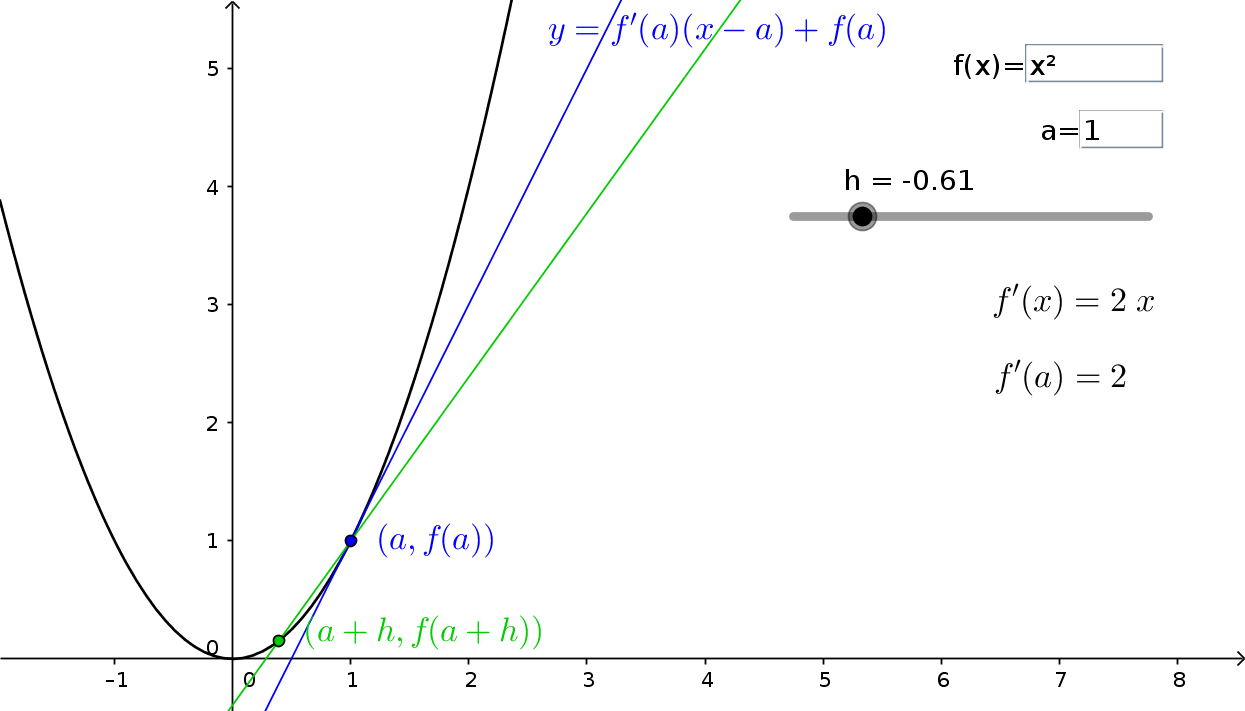
\includegraphics[width=12cm,keepaspectratio=true]{./01_05_snertill.png}
\end{center}



\subsection{Athugasemd: Hallatalan \protect\(\infty\protect\) er ekki leyfð}
\label{kafli03:athugasemd-hallatalan-er-ekki-leyf}
Við leyfum ekki \(f'(a) = \infty\) eða
\(f'(a) = -\infty\). Samanber
\(f(x) = x^{\frac 13}\) í \(a=0\),
\begin{equation*}
\begin{split}\lim_{h \to 0} \frac{f(0+h)-f(0)}h =
     \lim_{h \to 0} \frac{h^{\frac 13}}h =
    \lim_{h \to 0} h^{-\frac 23} = \infty.\end{split}
\end{equation*}
Hér ætti því jafna snertilsins að vera \(x=0\).

\noindent{\hspace*{\fill}\sphinxincludegraphics[width=12cm]{{01_x13}.png}\hspace*{\fill}}

Við viljum að snertillinn sé nálgun við graf fallsins fyrir \(x\) nálægt
\(a\), lóðrétt lína er gagnslaus nálgun því hún er ekki skilgreind sem
fall af \(x\).


\bigskip\hrule{}\bigskip



\section{Útvíkkun fyrir lokuð bil}
\label{kafli03:utvikkun-fyrir-loku-bil}
Ef fallið \(f\) er skilgreint á lokuðu bili þá getum við skilgreint
afleiðuna í endapunktunum með því að taka markgildi frá hægri/vinstri
eftir því sem við á.

\index{afleiða!hægri/vinstri}

\subsection{Skilgreining: Hægri/vinstri afleiða}
\label{kafli03:index-2}\label{kafli03:skilgreining-haegri-vinstri-afleia}\begin{enumerate}
\item {} 
\emph{Hægri afleiða falls} \(f\) \emph{í punkti} \(x\) er skilgreind
sem
\begin{equation*}
\begin{split}f_+'(x)=\lim_{h\rightarrow 0^+}\frac{f(x+h)-f(x)}{h}.\end{split}
\end{equation*}
\item {} 
\emph{Vinstri afleiða falls} \(f\) \emph{í punkti} \(x\) er
skilgreind sem
\begin{equation*}
\begin{split}f_-'(x)=\lim_{h\rightarrow 0^-}\frac{f(x+h)-f(x)}{h}.\end{split}
\end{equation*}
\end{enumerate}


\subsection{Setning}
\label{kafli03:id2}
Ef \(x\) er innri punktur í skilgreiningarsvæði fallsins \(f\)
þá er \(f\) diffranlegt í \(x\) þá og því að eins
\begin{equation*}
\begin{split}f_+'(x)=\lim_{h\rightarrow 0^+}\frac{f(x+h)-f(x)}{h}
=   f_-'(x)=\lim_{h\rightarrow 0^-}\frac{f(x+h)-f(x)}{h},\end{split}
\end{equation*}
og þá er \(f'(x)\) jafnt og markgildin hér fyrir ofan.

Þetta leiðir beint af skilgreiningunum hér á undan og
{\hyperref[kafli02:setning\string-hv\string-markgildi]{\sphinxcrossref{\DUrole{std,std-ref}{Setningu 2.2.5}}}}.

\index{afleiða!diffranlegt fall}

\subsection{Skilgreining: Diffranlegt fall}
\label{kafli03:skilgreining-diffranlegt-fall}\label{kafli03:index-3}
Látum \(f\) vera fall með skilgreiningarsvæði \(A\). Gerum ráð
fyrir að \(A\) sé sammengi endanlega margra bila. Við segjum að
fallið \(f\) sé \emph{diffranlegt} ef það er diffranlegt í öllum innri
punktum \(A\) og diffranlegt frá vinstri/hægri í jaðarpunktum
\(A\) eftir því sem við á.


\subsection{Ritháttur}
\label{kafli03:rithattur}
Afleiða falls \(f\) er ýmist táknuð með
\begin{equation*}
\begin{split}f', \qquad \frac {df}{dx}, \qquad D_x f \qquad \text{eða} \qquad Df.\end{split}
\end{equation*}
Ef við skrifum \(y=f(x)\) þá má einnig tákna hana með
\begin{equation*}
\begin{split}y', \qquad \frac {dy}{dx}, \qquad D_x y \qquad \text{eða} \qquad Dy.\end{split}
\end{equation*}

\subsection{Dæmi}
\label{kafli03:id3}
Fallið \(f(x) = \sqrt{x}\), \(f:[0,\infty[\to {{\mathbb  R}}\)
er diffranlegt á menginu \(]0,\infty[\) og afleiðan er gefin með
\(f'(x) = \frac 1{2\sqrt{x}} = \frac 12 x^{-1/2}\) þar. Hins vegar
er \(f\) ekki diffranlegt í \(x=0\) þrátt fyrir að fallgildið sé
vel skilgreint (og fallið samfellt frá hægri) þar.

Ef \(x>0\) þá fæst
\begin{equation*}
\begin{split}\begin{aligned}
  \lim_{h\to 0} \frac{\sqrt{x+h}-\sqrt{x}}h &=
  \lim_{h\to 0} \frac{(\sqrt{x+h}-\sqrt{x})(\sqrt{x+h}+\sqrt{x})}{h(\sqrt{x+h}+\sqrt{x})}\\
  &= \lim_{h\to 0} \frac{\sqrt{x+h}^2-\sqrt{x}^2}{h(\sqrt{x+h}+\sqrt{x})}\\
  &= \lim_{h\to 0} \frac{x+h-x}{h(\sqrt{x+h}+\sqrt{x})}\\
  &= \lim_{h\to 0} \frac{1}{\sqrt{x+h}+\sqrt{x}} = \frac{1}{2\sqrt{x}},\end{aligned}\end{split}
\end{equation*}
sem segir okkur að \(f'(x) = \frac 12 x^{-1/2}\).

Í vinstri endapunkti skilgreingarsvæðisins, \(x=0\), þá fæst hins
vegar
\begin{equation*}
\begin{split}\begin{aligned}
  \lim_{h\to 0^+} \frac{\sqrt{h}-\sqrt{0}}h &=
  \lim_{h\to 0^+} \frac{\sqrt{h}}h\\
  &= \lim_{h\to 0^+} \frac{1}{\sqrt{h}} = \infty,\end{aligned}\end{split}
\end{equation*}
sem sýnir að fallið er ekki diffranlegt frá hægri í \(x=0\).


\bigskip\hrule{}\bigskip



\section{Reiknireglur}
\label{kafli03:reiknireglur}

\subsection{Setning}
\label{kafli03:setning-3-3-1}\label{kafli03:id4}
Látum \(f\) og \(g\) vera föll sem eru diffranleg í punkti
\(x\). Þá eru föllin \(f+g,\ f-g, kf\) (þar sem \(k\) er
fasti) og \(fg\) diffranleg í punktinum \(x\), og ef
\(g(x)\neq 0\) þá eru föllin \(1/g\) og \(f/g\) líka
diffranleg í \(x\).

Eftirfarandi formúlur gilda um afleiður fallanna sem talin eru upp hér
að framan:
\begin{enumerate}
\item {} 
\((f+g)'(x)=f'(x)+g'(x)\)

\item {} 
\((f-g)'(x)=f'(x)-g'(x)\)

\item {} 
\((kf)'(x)=kf'(x)\), þar sem \(k\) er fasti

\item {} 
\((fg)'(x)=f'(x)g(x)+f(x)g'(x)\)

\item {} 
\(\displaystyle\Bigg(\frac{1}{g}\Bigg)'(x)=\frac{-g'(x)}{g(x)^2}\),
ef \(g(x)\neq 0\)

\item {} 
\(\displaystyle\Bigg(\frac{f}{g}\Bigg)'(x)=
\frac{f'(x)g(x)-f(x)g'(x)}{g(x)^2}\), ef \(g(x)\neq 0\)

\end{enumerate}


\subsection{Nokkrar afleiður}
\label{kafli03:setning-3-3-2}\label{kafli03:nokkrar-afleiur}\begin{enumerate}
\item {} 
\(\frac{d}{dx} c =  \lim_{h\to 0} \frac{c-c}h = 0\)

\item {} 
\(\frac{d}{dx} x =  \lim_{h\to 0} \frac{x+h-x}h = 1\)

\item {} 
\(\frac{d}{dx} x^2 = \lim_{h\to 0} \frac{x^2+2xh+h^2-x^2}h
= \lim_{h\to 0} \frac{2xh + h^2}h = \lim_{h\to 0} 2x+h= 2x\)

\end{enumerate}


\subsection{Setning}
\label{kafli03:id5}\label{kafli03:setning-3-3-3}\begin{equation*}
\begin{split}\frac{d}{dx} x^n = n x^{n-1}\end{split}
\end{equation*}
\textbf{Sönnun}

Sýnum þetta með þrepun.Tilfellið \(n=1\) er afgreitt hér að ofan
(3.3.2 (2)).
Gerum ráð fyrir að niðurstaðan gildi fyrir \(n\) og sýnum að þá
gildi hún einnig fyrir \(n+1\),
\begin{equation*}
\begin{split}\frac{d}{dx} x^{n+1} = \frac{d}{dx} (x\cdot x^n) =
    \left(\frac{d}{dx} x\right) x^n + x\frac{d}{dx} x^n
    = x^n + x\,
    \underbrace{n\, x^{n-1}}_\text{þ.f.}
    = (n+1) x^n.\end{split}
\end{equation*}

\subsection{Afleiður margliða}
\label{kafli03:afleiur-marglia}
Með því að nota setningarnar að ofan þá eigum við ekki í neinum
vandræðum með að diffra margliður. {\hyperref[kafli03:setning\string-3\string-3\string-1]{\sphinxcrossref{Setning 3.3.1}}} (i) segir
að við getum diffrað hvern lið fyrir sig, liður (iii) í sömu setningu
segir að við getum tekið fastana fram fyrir afleiðuna og loks segir
{\hyperref[kafli03:setning\string-3\string-3\string-3]{\sphinxcrossref{Setning 3.3.3}}} hvernig við diffrum \(x^n\).


\subsection{Dæmi: Afleiða margliðu}
\label{kafli03:daemi-afleia-margliu}
Finnum afleiðu margliðunnar \(p(x) = 4x^3-2x + 5\). Nú er
\begin{equation*}
\begin{split}\begin{aligned}
\frac{d}{dx} p(x)
&= \frac{d}{dx}4x^3 - \frac{d}{dx}2x + \frac{d}{dx}5 \\
&= 4\frac{d}{dx}x^3 -2\frac{d}{dx}x + \frac{d}{dx}5 =
4\cdot 3x^2 -2\cdot 1 + 0 = 12x^2-2\end{aligned}\end{split}
\end{equation*}
\index{keðjureglan}

\subsection{Setning: Keðjureglan}
\label{kafli03:kedjuregla}\label{kafli03:index-4}\label{kafli03:setning-kejureglan}
Gerum ráð fyrir að \(f\) og \(g\) séu föll þannig að \(g\)
er diffranlegt í \(x\) og \(f\) er diffranlegt í \(g(x)\).
Þá er samskeytingin \(f\circ g\) diffranleg í \(x\) og
\begin{equation*}
\begin{split}(f\circ g)'(x) = f'(g(x))\cdot g'(x).\end{split}
\end{equation*}

\subsection{Dæmi}
\label{kafli03:id7}
Skoðum föllin \(f(x) = \sqrt x\) og \(g(x) = 3x^5\). Bæði þessi föll eru
diffranleg og afleiðurnar eru \(f'(x) = \frac 12 x^{-1/2}\) og
\(g'(x) = 15x^4\). Afleiða samskeytingarinnar \(f\circ g\) er þá
samkvæmt keðjureglunni
\begin{equation*}
\begin{split}(f\circ g)'(x) = \frac 12 (3x^5)^{-1/2} \cdot 15x^4.\end{split}
\end{equation*}

\bigskip\hrule{}\bigskip



\section{Hærri afleiður}
\label{kafli03:haerri-afleiur}

\subsection{Skilgreining}
\label{kafli03:skilgreining}
Látum \(f\) vera fall. \emph{Afleiðan} \(f'\) er fall sem skilgreint er
í öllum punktum þar sem \(f\) er diffranlegt.

Ef fallið \(f'\) er diffranlegt í punkti \(x\) þá er afleiða
\(f'\) í punktinum \(x\) táknuð með \(f''(x)\) og kölluð
\textit{önnur afleiða} \(f\) í punktinum \(x\). Líta má á aðra afleiðu
\(f\) sem fall \(f''\) sem er skilgreint í öllum punktum þar sem
\(f'\) er diffranlegt.

Almennt má skilgreina \(n\)\emph{-tu afleiðu} \(f\), táknaða með
\(f^{(n)}\), þannig að í þeim punktum \(x\) þar sem fallið
\(f^{(n-1)}\) er diffranlegt þá er
\(f^{(n)}(x)=\frac{d}{dx}f^{(n-1)}(x)\).


\subsection{Dæmi}
\label{kafli03:id8}
Ef \(f(x)  = 3x^2\), þá er
\begin{equation*}
\begin{split}f'(x) = 3\frac{d}{dx}x^2 = 3\cdot 2x = 6x\end{split}
\end{equation*}
og
\begin{equation*}
\begin{split}f''(x) = \frac{d}{dx} 6x = 6.\end{split}
\end{equation*}

\subsection{Ritháttur}
\label{kafli03:id9}
Ritum \(y=f(x)\).

Þá má tákna fyrstu afleiðu \(f\) með
\begin{equation*}
\begin{split}y'= f'(x)=\frac{d}{dx}f(x)=D_xf(x)\ =\ D_x y= \frac{dy}{dx},\end{split}
\end{equation*}
aðra afleiðuna með
\begin{equation*}
\begin{split}\begin{aligned}
y'' &=
f''(x)=\frac{d}{dx}f'(x)=\frac{d}{dx}\frac{d}{dx}f(x)
= D^2_xf(x)= D^2_x y=\frac{d^2}{dx^2}f(x)=\frac{d^2 y}{dx^2}\end{aligned}\end{split}
\end{equation*}
og almennt \(n\)-tu afleiðuna
\begin{equation*}
\begin{split}\begin{aligned}
y^{(n)} &= f^{(n)}(x)=\frac{d}{dx}f^{(n-1)}(x)=
\frac{d}{dx}\Big(\frac{d^{n-1}}{dx^{n-1}}f(x)\Big) \\
&=D^n_xf(x)\ =\ D^n_x y
=\frac{d^n}{dx^n}f(x)
= \frac{d^n y}{dx^n}.\end{aligned}\end{split}
\end{equation*}
\begin{notice}{note}{Athugasemd:}
Venja er að rita \(f'''\) til að tákna þriðju afleiðu \(f\) en
afar sjaldgæft að \(f''''\) sé notað til að tákna fjórðu afleiðu
\(f\) og mun algengara að nota \(f^{(4)}\).
\end{notice}


\bigskip\hrule{}\bigskip



\section{Útgildi}
\label{kafli03:utgildi}\label{kafli03:id10}
\index{útgildi}\index{útgildi!hágildi}\index{útgildi!lággildi}

\subsection{Skilgreining: Útgildi}
\label{kafli03:index-5}\label{kafli03:skilgreining-utgildi}
Við segjum að fall \(f\) hafi \textit{staðbundið hágildi} í punktinum
\(x_0\) ef til er bil \((a,b)\) umhverfis \(x_0\), sem er
þannig að
\begin{equation*}
\begin{split}f(x) \leq f(x_0), \quad \text{ fyrir öll } x \in (a,b).\end{split}
\end{equation*}
Við segjum að fall \(f\) hafi \textit{staðbundið lággildi} í punktinum
\(x_0\) ef til er bil \((a,b)\) umhverfis \(x_0\), sem er
þannig að
\begin{equation*}
\begin{split}f(x) \geq f(x_0), \quad \text{ fyrir öll } x \in (a,b).\end{split}
\end{equation*}
Tölum um að fallið \(f\) hafi \textit{staðbundið útgildi} í punktinum
\(x_0\) ef það hefur staðbundið hágildi eða staðbundið lággildi þar.


\subsection{Setning}
\label{kafli03:setning-3-5-2}\label{kafli03:id11}
Ef fallið \(f\) hefur staðbundið útgildi í punktinum \(x_0\) og
er diffranlegt þá er \(f'(x_0)=0\).

\begin{DUlineblock}{0em}
\item[] 
\end{DUlineblock}

\textbf{Sönnun}

Gerum ráð fyrir að \(f\) hafi staðbundið hágildi í punktinum \(x_0\).
Þá er \(f(x_0)-f(x)\geq 0\) og ef \(x<x_0\),
þá fæst að  \(\frac{f(x_0)-f(x)}{x_0-x}\geq 0\). Þetta þýðir að
\begin{equation*}
\begin{split}\lim_{x \to x_0^-} = \frac{f(x_0) - f(x)}{x_0-x} \geq 0.
    \label{vinstri}\end{split}
\end{equation*}
Eins þá er \(f(x_0)-f(x)\geq 0\) og ef \(x_0<x\),
þá er \(\frac{f(x_0)-f(x)}{x_0-x} \leq 0\).
Þetta þýðir að
\begin{equation*}
\begin{split}\lim_{x \to x_0^+} = \frac{f(x_0) - f(x)}{x_0-x} \leq 0.
    \label{haegri}\end{split}
\end{equation*}
Við vitum að markgildið
\(\lim_{x\to x_0} \frac{f(x_0)-f(x)}{x_0-x}\) er til þar sem fallið
er diffranlegt, það þýðir að markgildin frá hægri og vinstri eru þau
sömu. Eina leiðin til þess að það samræmist hægri og vinstri markgildunum
hér að ofan er ef
\begin{equation*}
\begin{split}f'(x_0) = \lim_{x\to x_0} \frac{f(x_0)-f(x)}{x_0-x} = 0.\end{split}
\end{equation*}
\begin{DUlineblock}{0em}
\item[] 
\item[] 
\end{DUlineblock}

\begin{notice}{warning}{Aðvörun:}
Þó að \(f'(a)=0\) þá er ekki víst að \(a\) sé staðbundið útgildi.

Til dæmis þá hefur fallið \(f(x) = x^3\) ekkert staðbundið útgildi
þrátt fyrir að \(f'(0) = 0\) (\(f'(x) = 3x^2\)).
\end{notice}


\bigskip\hrule{}\bigskip



\section{Hornaföll og afleiður þeirra}
\label{kafli03:hornafoll-og-afleiur-eirra}

\subsection{Setning}
\label{kafli03:id12}\begin{enumerate}
\item {} 
\(\displaystyle\lim_{x\rightarrow 0}\frac{\sin x}{x}=1\)

\item {} 
\(\displaystyle\lim_{x\rightarrow 0}\frac{\cos x-1}{x}=0\)

\item {} 
\(\displaystyle\frac{d}{dx}\sin x=\cos x\)

\item {} 
\(\displaystyle\frac{d}{dx}\cos x=-\sin x\)

\item {} 
\(\displaystyle\frac{d}{dx}\tan x=\frac{1}{\cos^2 x}=1+\tan^2 x\)

\end{enumerate}


\bigskip\hrule{}\bigskip



\section{Meðalgildissetningin}
\label{kafli03:mealgildissetningin}
\index{setning Rolle}

\subsection{Setning Rolle}
\label{kafli03:rolle}\label{kafli03:index-6}\label{kafli03:setning-rolle}
Látum \(g:[a,b]\rightarrow{{\mathbb  R}}\) vera samfellt fall. Gerum
ráð fyrir að \(g\) sé diffranlegt í öllum punktum í bilinu
\((a,b)\). Ef \(g(a)=g(b)\) þá er til punktur \(c\) á bilinu
\((a,b)\) þannig að \(g'(c)=0\).

\textbf{Sönnun}

Ef \(g(x)=c\) er fasti, þá er \(g'(x)=0\). Ef hins vegar
\(g\) er ekki fasti þá er til \(x \in (a,b)\) þannig að
\(g(x)\neq g(a)\), gerum ráð fyrir að \(g(x)>g(a)\)
(tilfellið ef \(g(x)<g(a)\) gengur nánast eins fyrir sig).
Samkvæmt Há- og lággildislögmálinu
þá tekur fallið \(g\) sitt hæsta
gildi í punkti \(c\) á bilinu \([a,b]\).Þar sem
\(g(c)\geq g(x) >  g(a) = g(b)\) þá getur \(c\) hvorki verið
\(a\) né \(b\).
Þar sem \(c\)
er útgildi þá segir {\hyperref[kafli03:setning\string-3\string-5\string-2]{\sphinxcrossref{Setning 3.5.2}}} að \(g'(c)=0\).

\index{meðalgildissetningin}

\subsection{Meðalgildissetningin}
\label{kafli03:id13}\label{kafli03:index-7}
Látum \(f:[a,b]\rightarrow{{\mathbb  R}}\) vera samfellt fall. Gerum
ráð fyrir að \(f\) sé diffranlegt í öllum punktum í bilinu
\((a,b)\). Þá er til punktur \(c\) í bilinu \((a,b)\) þannig
að
\begin{equation*}
\begin{split}\frac{f(b)-f(a)}{b-a}=f'(c).\end{split}
\end{equation*}
\textbf{Sönnun}

Skilgreinum nýtt fall
\begin{equation*}
\begin{split}h(x)=f(x)-\left(f(a)+ \frac{f(b)-f(a)}{b-a}(x-a)\right).\end{split}
\end{equation*}
Athugið að \(h\) er bara \(f\) mínus línan sem liggur í gegnum
\((a,f(a))\) og \((b,f(b))\). Þetta þýðir að \(h\) er diffranlegt
og að \(h(a)=h(b)=0\). Þá gefur Setning Rolle að til er \(c\) þannig að
\(h'(c)=0\).

Nú er
\begin{equation*}
\begin{split}h'(x) = f'(x) - \left(0+\frac{f(b)-f(a)}{b-a}(1-0)\right)
= f'(x) - \frac{f(b)-f(a)}{b-a}\end{split}
\end{equation*}
þannig að
\begin{equation*}
\begin{split}0 = h'(c) = f'(c) - \frac{f(b)-f(a)}{b-a},\end{split}
\end{equation*}
eða
\begin{equation*}
\begin{split}f'(c) = \frac{f(b)-f(a)}{b-a}.\end{split}
\end{equation*}
\begin{notice}{note}{Athugasemd:}
Niðurstöðuna úr \textit{meðalgildissetningunni} má orða svona:

Í einhverjum punkti á bilinu er stundarbreytingin jöfn meðalbreytingunni
yfir allt bilið.
\end{notice}

\index{meðalgildissetningin}

\subsection{Alhæfða meðalgildissetningin}
\label{kafli03:alhaefa-mealgildissetningin}\label{kafli03:index-8}
Gerum ráð fyrir að föllin \(f\) og \(g\) séu samfelld á lokaða
bilinu \([a,b]\) og diffranleg á opna bilinu \((a,b)\). Gerum
auk þess ráð fyrir að fyrir allar tölur \(x\) í \((a,b)\) sé
\(g'(x)\neq 0\). Þá er til tala \(c\in (a,b)\) þannig að
\begin{equation*}
\begin{split}\frac{f(b)-f(a)}{g(b)-g(a)}=\frac{f'(c)}{g'(c)}.\end{split}
\end{equation*}

\bigskip\hrule{}\bigskip



\section{Vaxandi og minnkandi föll}
\label{kafli03:vaxandi-og-minnkandi-foll}\label{kafli03:vaxandiminnkandi}
\index{fall!vaxandi/minnkandi}

\subsection{Skilgreining: Vaxandi/minnkandi}
\label{kafli03:index-9}\label{kafli03:skilgreining-vaxandi-minnkandi}
Fall \(f\) er \emph{vaxandi} á bili \((a,b)\) ef um
alla punkta \(x_1\) og \(x_2\) á \((a,b)\) þannig að
\(x_1 < x_2\) gildir að
\begin{equation*}
\begin{split}f(x_1) \leq f(x_2).\end{split}
\end{equation*}
Fall \(f\) er \emph{stranglega vaxandi} á bili \((a,b)\)
ef um alla punkta \(x_1\) og \(x_2\) á \((a,b)\) þannig að
\(x_1 < x_2\) gildir að
\begin{equation*}
\begin{split}f(x_1) < f(x_2).\end{split}
\end{equation*}
Fall \(f\) er \emph{minnkandi} á bili \((a,b)\) ef um
alla punkta \(x_1\) og \(x_2\) á \((a,b)\) þannig að
\(x_1 < x_2\) gildir að
\begin{equation*}
\begin{split}f(x_1) \geq f(x_2).\end{split}
\end{equation*}
Fall \(f\) er \emph{stranglega minnkandi} á bili
\((a,b)\) ef um alla punkta \(x_1\) og \(x_2\) á
\((a,b)\) þannig að \(x_1 < x_2\) gildir að
\begin{equation*}
\begin{split}f(x_1) > f(x_2).\end{split}
\end{equation*}
\begin{notice}{note}{Athugasemd:}
Kennslubókin notar \emph{nondecreasing/nonincreasing} fyrir vaxandi/minnkandi og
\emph{increasing/decreasing} fyrir stranglega vaxandi/minnkandi.

Einnig þekkist að nota \emph{increasing/decreasing} og \emph{strictly increasing/decreasing}.
Til dæmis er það gert á \href{https://en.wikipedia.org/wiki/Monotonic\_function}{Wikipedia: Monotonic functions} (https://en.wikipedia.org/wiki/Monotonic\_function).
\end{notice}


\subsection{Setning}
\label{kafli03:vaxandieoae}\label{kafli03:id15}
Látum \(f\) vera diffranlegt fall. Þá er \(f\) vaxandi þá og því
aðeins að \(f' \geq 0\).

\textbf{Sönnun}

Byrjum á að gera ráð fyrir að fallið sé vaxandi. Festum punkt \(x\) og
sýnum að \(f'(x)\geq 0\). Þar sem \(f\) er vaxandi þá gildir fyrir
sérhvert \(h>0\) að
\begin{equation*}
\begin{split}\frac{f(x+h)-f(x)}{h} \geq 0\end{split}
\end{equation*}
Þá gildir einnig um markgildið \(\lim_{h\to 0^+} \frac{f(x+h)-f(x)}h \geq 0\).

Ef hins vegar \(h<0\) þá er \(x+h < x\) og því
\(f(x+h)<f(x)\). Þetta gefur að
\begin{equation*}
\begin{split}\frac{f(x+h)-f(x)}h \geq 0\end{split}
\end{equation*}
sem þýðir að \(\lim_{h\to 0^-} \frac{f(x+h)-f(x)}h \geq 0\). Og þar af leiðandi
er \(f'(x) = \lim_{h\to 0} \frac{f(x+h)-f(x)}h \geq 0\).


\bigskip\hrule{}\bigskip


Gerum nú ráð fyrir \(f'\geq 0\) og sýnum að þá sé fallið vaxandi.
Festum tvo punkta \(x_1 < x_2\). Ef \(f(x_1) > f(x_2)\), það er
\(f(x_2)-f(x_1)<0\)
þá er
\begin{equation*}
\begin{split}\frac{f(x_2)-f(x_1)}{x_2-x_1} < 0.\end{split}
\end{equation*}
Samkvæmt meðalgildissetningunni þá er til punktur \(¢\) á bilinu \([x_1,x_2]\)
þar sem afleiðan tekur þetta gildi, en það er í mótsögn við að  \(f'(c)\geq 0\).


\subsection{Setning}
\label{kafli03:minnkandieoae}\label{kafli03:id16}
Látum \(f\) vera diffranlegt fall. Þá er \(f\) minnkandi þá og
því aðeins að \(f' \leq 0\).


\subsection{Setning}
\label{kafli03:id17}
Látum \(f\) vera diffranlegt fall. Ef \(f'>0\) þá er \(f\)
stranglega vaxandi.


\subsection{Setning}
\label{kafli03:id18}
Látum \(f\) vera diffranlegt fall. Ef \(f'<0\) þá er \(f\)
stranglega minnkandi.

\begin{notice}{warning}{Aðvörun:}
Diffranlegt fall getur verið stranglega vaxandi/minnkandi án þess að
afleiðan sé alls staðar stærri/minni en 0. Til dæmis er afleiða \(f(x)=x^3\) jöfn 0 í
\(x=0\) en fallið er stranglega vaxandi á öllum rauntalnaásnum.
\end{notice}


\subsection{Afleiður fastafalla}
\label{kafli03:afleiur-fastafalla}
Við vitum að ef \(f\) er fasti, það er \(f(x)=c\), þá er
\(f'(x)=0\) fyrir öll \(x\).

Nú fáum við einnig eftirfarandi út frá Setningum {\hyperref[kafli03:vaxandieoae]{\sphinxcrossref{\DUrole{std,std-ref}{3.8.2}}}} og {\hyperref[kafli03:minnkandieoae]{\sphinxcrossref{\DUrole{std,std-ref}{3.8.3}}}}:

Ef \(f\) er diffranlegt fall á bili \(I\) sem er þannig að
\(f'(x) = 0\) á \(I\), þá er \(f\) fasti,
þ.e. \(f(x) = c\) fyrir öll \(x\in I\).


\bigskip\hrule{}\bigskip



\section{Fólgin diffrun}
\label{kafli03:folgin-diffrun}

\subsection{Dæmi}
\label{kafli03:id19}
Jafna hrings með geisla 1 er \(x^2+y^2=1\). Við vitum að hægt er að
skrifa efri og neðri helminga hans sem föll af \(y\), annars vegar
\(y=\sqrt{1-x^2}\) og hins vegar \(y=-\sqrt{1-x^2}\). Ef við
viljum finna snertil við hringinn getum við notað þessi föll. En þar sem
við vitum að hægt er að skrifa \(y\) sem fall af \(x\) þá getum
við einnig diffrað jöfnu hringsins beint með aðstoð keðjureglunnar,
\begin{equation*}
\begin{split}\begin{aligned}
\frac{d}{dx}(x^2+y^2) &=& \frac{d}{dx} 1\\
    2x + 2y\frac{dy}{dx} &=& 0\\
    y\frac{dy}{dx} &=& -x\\
    \frac{dy}{dx} &=& -\frac xy.\end{aligned}\end{split}
\end{equation*}
\noindent{\hspace*{\fill}\sphinxincludegraphics[width=12cm]{{11_hringur}.png}\hspace*{\fill}}


\subsection{Setning: Andhverfusetningin}
\label{kafli03:setning-andhverfusetningin}
Látum feril vera gefinn með \(F(x,y) =0\), þar sem \(F\) er
diffranlegt í bæði \(x\) og \(y\). Í punktum þar sem ferillinn
er ekki lóðréttur (þ.e. \(\frac{d}{dy}F \neq 0\)) þá er hægt að
skrifa \(y\) sem fall af \(x\) og þá fæst af keðjureglunni að
\begin{equation*}
\begin{split}\frac{d}{dx} F(x,y) + \frac{d}{dy}F(x,y) \frac{dy}{dx} = 0,\end{split}
\end{equation*}
þ.e.
\begin{equation*}
\begin{split}\frac{dy}{dx} = -\frac{\frac{d}{dx} F(x,y)}{\frac{d}{dy} F(x,y)}.\end{split}
\end{equation*}
Sjá \url{https://en.wikipedia.org/wiki/Inverse\_function\_theorem}


\subsection{Með öðrum orðum}
\label{kafli03:me-orum-orum}
Það kemur á sama stað niður að einangra \(y=f(x)\), ef það er
mögulegt, og finna \(y'\) með því að diffra, eins og að diffra
\(F(x,y)=0\) og einangra svo \(y'=\frac{dy}{dx}\).


\subsection{Vinnulag}
\label{kafli03:vinnulag}\begin{enumerate}
\item {} 
Diffrum beggja vegna jöfnuna með tilliti til \(x\), og lítum á
\(y\) sem fall af \(x\) sem við diffrum með aðstoð
keðjureglunnar (og gleymum ekki \(y'\))

\item {} 
Einangrum \(y'\)

\item {} 
Skiptum \(y\) út fyrir \(f(x)\).

\end{enumerate}


\subsection{Setning: Hagnýting á fólginni diffrun}
\label{kafli03:setning-hagnyting-a-folginni-diffrun}
Ef \(n\) og \(m\) eru heilar tölur þá er
\begin{equation*}
\begin{split}\frac{d}{dx} x^{\frac nm} = \frac nm x^{\frac nm -1}.\end{split}
\end{equation*}
\textbf{Sönnun}

Punktar á grafi fallsins \(x^{n/m}\) ákvarðast af jöfnunni \(y=x^{n/m}\), það er
\(y^m = x^n\). Skilgreinum því
\begin{equation*}
\begin{split}F(x,y) = x^n-y^m\end{split}
\end{equation*}
Þar sem \(\frac d{dx} F(x,y) = nx^{n-1}\) og
\(\frac d{dy} F(x,y) = -my^{m-1}\) þá fæst að
\begin{equation*}
\begin{split}\begin{aligned}
y' &= \frac {d}{dx} y =
- \frac{n x^{n-1}}{-m y^{m-1}} =
\frac{n x^{n-1}}{m (x^{\frac nm})^{m-1}} \\
&= \frac nm x^{(n-1) - \frac nm(m-1)}
= \frac nm x^{n-1-n+\frac nm} = \frac nm x^{\frac nm -1}. \end{aligned}\end{split}
\end{equation*}

\bigskip\hrule{}\bigskip


\index{fall!andhverfa}

\section{Andhverf föll}
\label{kafli03:index-10}\label{kafli03:andhverf-foll}
Rifjum upp að gagntæk vörpun \(f:X\to Y\) hefur andhverfu
\(f^{-1}:Y\to X\) sem uppfyllir að
\begin{equation*}
\begin{split}y=f(x)\qquad\mbox{þá og því aðeins að}\qquad x=f^{-1}(y).\end{split}
\end{equation*}
Sjá {\hyperref[kafli01:andhverfa]{\sphinxcrossref{\DUrole{std,std-ref}{kafla 1.4}}}}.


\subsection{Athugasemd}
\label{kafli03:athugasemd}
Látum \(f:X \to Y\) vera fall sem skilgreint er á mengi \(X\). Gerum ráð
fyrir að \(f\) sé eintækt. Með því að einskorða bakmengi \(f\) við
myndmengið \(\tilde Y = f(X)\) þá verður \(f:X\to \tilde Y\) gagntækt fall.
Þá er til andhverfa \(f^{-1}:\tilde Y \to X\) sem uppfyllir
\begin{equation*}
\begin{split}y=f(x)\qquad\mbox{þá og því aðeins að}\qquad x=f^{-1}(y).\end{split}
\end{equation*}

\subsection{Setning}
\label{kafli03:id20}
Fall sem er strangt vaxandi eða strangt minnkandi er eintækt og á sér
því andhverfu.


\subsection{Eiginleikar}
\label{kafli03:eiginleikar}\begin{enumerate}
\item {} 
\(y=f^{-1}(x)\) þá og því aðeins að \(x=f(y)\).

\item {} 
Skilgreingarsvæði \(f\) er myndmengi \(f^{-1}\).

\item {} 
Myndmengi \(f^{-1}\) er jafnt skilgreiningarsvæði \(f\).

\item {} 
\(f^{-1}(f(x))=x\) fyrir öll \(x\) í skilgreiningarsvæði
\(f\).

\item {} 
\(f(f^{-1}(x))=x\) fyrir öll \(x\) í skilgreiningarsvæði
\(f^{-1}\).

\item {} 
\((f^{-1})^{-1}(x)=f(x)\) fyrir öll \(x\) í
skilgreiningarsvæði \(f\), alltsvo \((f^{-1})^{-1}=f\).

\item {} 
Graf \(f^{-1}\) er speglun á grafi \(f\) um línuna
\(y=x\).

\end{enumerate}

\index{afleiða!andhverfa}

\subsection{Setning: Afleiða andhverfunnar}
\label{kafli03:setning-afleia-andhverfunnar}\label{kafli03:index-12}
Gerum ráð fyrir að fall \(f\) hafi andhverfu \(f^{-1}\). Látum
\(x\) vera á skilgreiningarsvæði \(f\) og gerum ráð fyrir að
\(f\) sé diffranlegt í punktinum \(f^{-1}(x)\) og að
\(f'(f^{-1}(x))\neq 0\). Þá er \(f^{-1}\) diffranlegt í
punktinum \(x\) og
\begin{equation*}
\begin{split}\left(f^{-1}\right)'(x)=\frac{1}{f'(f^{-1}(x))}\end{split}
\end{equation*}
\begin{notice}{note}{Athugasemd:}
Setningin segir okkur sér í lagi að láréttur snertill við \(f\)
svarar til lóðrétts snertils við \(f^{-1}\).
\end{notice}


\bigskip\hrule{}\bigskip



\section{Línulegar nálganir}
\label{kafli03:linulegar-nalganir}

\subsection{Staðbundnar nálganir}
\label{kafli03:stabundnar-nalganir}
Skoðum diffranlegt fall \(f\) í grennd um fastann punkt
\(a\). Látum \(x\) vera punkt í grennd um \(a\)
Ef graf fallsins er ekki ,,mjög
sveigt” þá er snertillinn við \((a,f(a))\) næstum samsíða
sniðlinum gegnum \((a,f(a))\) og \((x,f(x))\).
Það þýðir að
\begin{equation*}
\begin{split}\begin{aligned}
     \frac{f(x)-f(a)}{x-a} &\approx f'(a),\\
     f(x)-f(a) &\approx  f'(a)(x-a),\\
     f(x) &\approx f'(x)(x-a) + f(a).
\end{aligned}\end{split}
\end{equation*}
\begin{notice}{warning}{Aðvörun:}
Athugið að hér er \(a\) fast en \(x\) breytist.
\end{notice}

\begin{notice}{note}{Athugasemd:}
Einnig er hægt að skrifa þetta á eftirfarandi hátt.
Skilgreinum \(x\) = a + Delta x{}` og
\(\Delta y = f(x) - f(a)\) þá þýðir þetta að
\(\Delta y \approx \Delta x f'(a)\).

Það er, breytingin á fallgildinum er um það bil breytingin í
breytunni margfaldað við afleiðuna í punktinum.
\end{notice}


\subsection{Skilgreining: Línuleg nálgun}
\label{kafli03:skilgreining-linuleg-nalgun}
Línuleg nálgun á falli \(f\) nálægt \(a\), eða 1. stigs Taylor
margliða \(f\) í \(a\), er gefin með
\(P_1(x)=f(a)+f'(a)(x-a)\).


\subsection{Setning: Skekkjumat}
\label{kafli03:setning-skekkjumat}
Skekkjan í nálguninni \(E_1(x)=f(x)-P_1(x)\) uppfyllir að til er
tala \(X \in (a,x)\) þannig að
\begin{equation*}
\begin{split}E_1(x)=\frac{f''(X)}{2}(x-a)^2.\end{split}
\end{equation*}

\subsection{Skekkjumat fyrir línulegar nálganir}
\label{kafli03:skekkjumat-fyrir-linulegar-nalganir}
Gerum ráð fyrir að \(f''(t)\) sé skilgreint fyrir öll \(t\) í
opnu bili sem inniheldur bæði \(a\) og \(x\). Gerum enn fremur
ráð fyrir að \(m\) og \(M\) séu tölur þannig að fyrir öll
\(t\in (a, x)\) gildi að \(m\leq f''(t)\leq M\). Þá er
\begin{equation*}
\begin{split}\frac{m}{2}(x-a)^2\leq E_1(x)
=\frac{f''(X)}{2}(x-a)^2\leq \frac{M}{2}(x-a)^2,\end{split}
\end{equation*}
sem gefur að
\begin{equation*}
\begin{split}f(a)+f'(a)(x-a)+\frac{m}{2}(x-a)^2\leq f(x)
\leq f(a)+f'(a)(x-a)+\frac{M}{2}(x-a)^2.\end{split}
\end{equation*}

\bigskip\hrule{}\bigskip



\section{Taylormargliður}
\label{kafli03:taylormargliur}
Línuleg nálgun á falli er ekkert annað en nálgun með fyrsta stigs
margliðu.

Spurningin er því hvort hægt sé að nota margliður af hærra stigi og fá
þá betri nálgun?

Hvernig er 0. stigs nálgun á falli?

\index{Taylor margliða}

\subsection{Skilgreining: Taylormargliða}
\label{kafli03:index-13}\label{kafli03:skilgreining-taylormarglia}
Gerum ráð fyrir að fall \(f\) sé diffranlegt \(n\) sinnum í
punkti \(a\), þ.e.a.s. við gerum ráð fyrir að \(n\)-ta afleiðan
\(f^{(n)}(a)\) sé skilgreind. \emph{Taylor margliða} af \(n\)-ta
stigi fyrir \(f\) um \(x=a\) (oft líka sagt með \emph{miðju} í
\(a\)) er margliðan
\begin{equation*}
\begin{split}\begin{gathered}
    P_n(x)=f(a)+f'(a)(x-a)+\frac{f''(a)}{2}(x-a)^2+ \\
    \frac{f'''(a)}{3!}(x-a)^3+\cdots+\frac{f^{(n)}(a)}{n!}(x-a)^n.\end{gathered}\end{split}
\end{equation*}
Talað er um \(n\)-ta stigs Taylor nálgun þegar gildið \(P_n(x)\)
er notað sem nálgun fyrir \(f(x)\).

Skekkjan í nálguninni (munurinn á réttu fallgildi og nálgunargildi) er
táknaður með
\begin{equation*}
\begin{split}E_n(x)=f(x)-P_n(x).\end{split}
\end{equation*}

\subsection{Skekkjumat fyrir Taylor margliður}
\label{kafli03:skekkjumat-fyrir-taylor-margliur}
Gerum ráð fyrir að \(n+1\)-afleiðan \(f^{(n+1)}(t)\) sé
skilgreind fyrir öll \(t\) í opnu bili sem inniheldur bæði \(a\)
og \(x\). Þá er til tala \(X\) á milli \(a\) og \(x\)
þannig að
\begin{equation*}
\begin{split}E_n(x)=\frac{f^{(n+1)}(X)}{(n+1)!}(x-a)^{n+1}.\end{split}
\end{equation*}
Því má rita
\begin{equation*}
\begin{split}\begin{aligned}
f(x)
=&f(a)+f'(a)(x-a)+\frac{f''(a)}{2}(x-a)^2+ \\
 & \cdots+\frac{f^{(n)}(a)}{n!}(x-a)^n+E_n(x)\\
=&f(a)+f'(a)(x-a)+\frac{f''(a)}{2}(x-a)^2+\\
 & \cdots+\frac{f^{(n)}(a)}{n!}(x-a)^n
  +\frac{f^{(n+1)}(X)}{(n+1)!}(x-a)^{n+1}.\end{aligned}\end{split}
\end{equation*}
\begin{notice}{warning}{Aðvörun:}
Yfirleitt er engin leið til þess að finna \(X\).
Hins vegar getum við haft gagn af skekkjumatinu ef
við höfum mat á \(f^{(n+1)}\).
\end{notice}


\subsection{Fylgisetning}
\label{kafli03:fylgisetning}
Gerum ráð fyrir að \(f\) sé \(n+1\) diffranlegt á bili sem
inniheldur bæði \(a\) og \(x\). Gerum enn fremur ráð fyrir að
\(m\) og \(M\) séu tölur þannig að fyrir öll \(t\in (a, x)\)
gildi að \(m\leq f^{(n+1)}(t)\leq M\). Þá er
\begin{equation*}
\begin{split}P_n(x) + \frac{m}{(n+1)!}(x-a)^{n+1} \leq f(x)
\leq P_n(x) + \frac{M}{(n+1)!}(x-a)^{n+1}.\end{split}
\end{equation*}
\index{O-ritháttur}

\subsection{Skilgreining: O}
\label{kafli03:index-14}\label{kafli03:skilgreining-o}
Við ritum
\begin{equation*}
\begin{split}f(x)=O(u(x)) \mbox{ þegar } x\rightarrow a\end{split}
\end{equation*}
ef til er fasti \(K\) og tala \(\delta>0\) þannig að
\begin{equation*}
\begin{split}|f(x)|<K|u(x)|\quad\mbox{ fyrir öll}\quad x\in(a-\delta, a+\delta).\end{split}
\end{equation*}
Einnig ritað
\begin{equation*}
\begin{split}f(x)=g(x)+O(u(x)) \mbox{ þegar }x\rightarrow a\end{split}
\end{equation*}
ef \(f(x)-g(x)=O(u(x))\) þegar \(x\rightarrow a\).

Tilgangur þessa ritháttar er að skilgreina tól sem getur sagt okkur
hversu hratt \(f\) stefnir á markgildið þegar \(x\to a\).


\subsection{Athugasemd}
\label{kafli03:id21}
Við sjáum að
\begin{equation*}
\begin{split}f(x) = P_n(x) + O((x-a)^{n+1}) \mbox{ þegar } x\rightarrow a,\end{split}
\end{equation*}
því hægt er að nota \(K = \frac{\max\{-m,M\}}{(n+1)!}\) í skilgreiningunni
hér á undan.


\subsection{Setning}
\label{kafli03:id22}
Gerum ráð fyrir að \(Q_n(x)\) sé margliða af stigi ekki hærra en
\(n\). Ef \(f(x)=Q_n(x)+O((x-a)^{n+1})\) þegar
\(x\rightarrow a\) þá er \(Q_n(x)=P_n(x)\) þar sem
\(P_n(x)\) er \(n\)-ta stigs Taylor margliða \(f\) með miðju
í \(a\).

Með öðrum orðum, \(P_n\) er sú margliða af stigi \(\leq n\) sem
nálgar \(f\) best.

\index{regla l’Hôpital}

\bigskip\hrule{}\bigskip



\section{Regla l’Hôpital}
\label{kafli03:regla-lhopital}\label{kafli03:index-15}

\subsection{Regla l’Hôpital, einhliða útgáfa}
\label{kafli03:regla-lhopital-einhlia-utgafa}
Gerum ráð fyrir að föllin \(f\) og \(g\) séu diffranleg á opnu
bili \((a,
b)\) og að \(g'(x)\neq 0\) fyrir öll \(x\in (a, b)\). Gerum enn
fremur ráð fyrir að
\begin{equation*}
\begin{split}\lim_{x\rightarrow a^+}f(x)=0, \quad \lim_{x\rightarrow a^+}g(x)=0
\quad\mbox{og}\quad \lim_{x\rightarrow a^+}\frac{f'(x)}{g'(x)}=L.\end{split}
\end{equation*}
(Hér má \(L\) vera rauntala, \(\infty\) eða \(-\infty\).)

Þá er
\begin{equation*}
\begin{split}\lim_{x\rightarrow a^+}\frac{f(x)}{g(x)}=L.\end{split}
\end{equation*}
Eins má skoða markgildi frá vinstri \(x\to a^-\).

Þar sem \(\lim_{x\rightarrow a^+}f(x)=\lim_{x\rightarrow a^+}g(x)=0\)
þá getum við gert ráð fyrir að \(f\) og \(g\) séu samfelld á
bilinu \([a,b)\) og taki gildið 0 í \(a\).

Þá fæst af alhæfðu meðalgildissetningunni fyrir sérhvert \(x\in (a,b)\)
að til er \(c \in (a,x)\) þannig að
\begin{equation*}
\begin{split}\frac{f(x)}{g(x)} = \frac{f(x)-f(a)}{g(x)-g(0)} = \frac{f'(c)}{g'(c)}\end{split}
\end{equation*}
Þegar \(x \to a^+\) þá gildir einnig að \(c \to a^+\) því
\(c\) er klemmt á milli \(a\) og \(x\).
Þar sem markgildið
\begin{equation*}
\begin{split}\lim_{c\to a^+} \frac{f'(c)}{g'(x)} = L\end{split}
\end{equation*}
er til, þá er markgildið \(\lim_{x\rightarrow a^+}\frac{f(x)}{g(x)}\)
einnig til og er jafnt og \(L\).


\subsection{Regla l’Hôpital}
\label{kafli03:id23}
Gerum ráð fyrir að föllin \(f\) og \(g\) séu diffranleg á bilum
\((x_1, a)\) og \((a, x_2)\) og að \(g'(x)\neq 0\) fyrir öll
\(x\) í þessum bilum.
Gerum enn fremur ráð fyrir að
\begin{equation*}
\begin{split}\lim_{x\rightarrow a}f(x)=0, \quad \lim_{x\rightarrow a}g(x)=0
\quad\mbox{og}\quad \lim_{x\rightarrow a}\frac{f'(x)}{g'(x)}=L.\end{split}
\end{equation*}
(Hér má \(L\) vera rauntala, \(\infty\) eða \(-\infty\).)

Þá er
\begin{equation*}
\begin{split}\lim_{x\rightarrow a}\frac{f(x)}{g(x)}=L.\end{split}
\end{equation*}

\subsection{Dæmi}
\label{kafli03:id24}
Við höfum áður séð að \(\lim_{x\to 0} \sin(x)/x = 1\).
Skoðum hvernig hægt er að sýna þetta með lítilli fyrirhöfn og reglu l’Hôpital.

Sjáum að \(f(x) = \sin(x)\) og \(g(x)\) eru diffranleg í grennd um 0
og að \(g'(x) = 1 \neq 0\). Þá fæst að
\begin{equation*}
\begin{split}\lim_{x \to 0} \frac{\sin(x)}{x} = \lim_{x \to 0} \frac{\cos(x)}{1} = 1.\end{split}
\end{equation*}

\subsection{Regla l’Hôpital, \protect\(\infty\protect\)-útgáfa}
\label{kafli03:regla-lhopital-utgafa}
Gerum ráð fyrir að föllin \(f\) og \(g\) séu diffranleg á bilum
\((x_1, \infty)\) og að \(g'(x)\neq 0\) fyrir öll
\(x\in (x_1, \infty)\). Gerum enn fremur ráð fyrir að
\begin{equation*}
\begin{split}\lim_{x\rightarrow \infty}f(x)=0, \quad \lim_{x\rightarrow \infty}g(x)=0
\quad\mbox{og}\quad \lim_{x\rightarrow \infty}\frac{f'(x)}{g'(x)}=L.\end{split}
\end{equation*}
(Hér má \(L\) vera rauntala, \(\infty\) eða \(-\infty\).)

Þá er
\begin{equation*}
\begin{split}\lim_{x\rightarrow \infty}\frac{f(x)}{g(x)}=L.\end{split}
\end{equation*}

\subsection{Regla l’Hôpital, útgáfa 4}
\label{kafli03:regla-lhopital-utgafa-4}
Gerum ráð fyrir að föllin \(f\) og \(g\) séu diffranleg á bilum
\((x_1, a)\) og \((a, x_2)\) og að \(g'(x)\neq 0\) fyrir öll
\(x\) í þessum bilum. Gerum enn fremur ráð fyrir að
\begin{equation*}
\begin{split}\lim_{x\rightarrow a}g(x)=\pm\infty
\quad\mbox{og}\quad \lim_{x\rightarrow a}\frac{f'(x)}{g'(x)}=L.\end{split}
\end{equation*}
(Hér má \(L\) vera rauntala, \(\infty\) eða \(-\infty\).)

Þá er
\begin{equation*}
\begin{split}\lim_{x\rightarrow a}\frac{f(x)}{g(x)}=L.\end{split}
\end{equation*}

\chapter{Torræð föll}
\label{kafli04:torrae-foll}\label{kafli04::doc}
\begin{notice}{note}{Athugasemd:}
\textbf{Nauðsynleg undirstaða}
\begin{itemize}
\item {} 
hornaföll

\item {} 
{\hyperref[kafli01:andhverfa]{\sphinxcrossref{\DUrole{std,std-ref}{andhverfur falla}}}}

\end{itemize}
\end{notice}

\emph{We are stuck with technology when what we really want is just stuff that works.}

- Douglas Adams, The Salmon of Doubt


\bigskip\hrule{}\bigskip



\section{Náttúrlegi logrinn}
\label{kafli04:natturlegi-logrinn}
\index{logri}

\subsection{Skilgreining: Náttúrlegi logrinn}
\label{kafli04:index-0}\label{kafli04:skilgreining-natturlegi-logrinn}
Látum \(A_{x_0}\) tákna flatarmál svæðisins sem afmarkast af
\(x\)-ás, grafinu \(y=\frac{1}{x}\) og línunum \(x=1\) og
\(x=x_0\). Þá skilgreinum við \textit{náttúrlega logrann} með formúlunni
\begin{equation*}
\begin{split}\ln x_0 =\left\{\begin{array}{ll}
A_{x_0} & \mbox{ef }x_0 \geq 1,\\
-A_{x_0} & \mbox{ef }0<x_0<1.
\end{array}
\right.\end{split}
\end{equation*}

\begin{center}
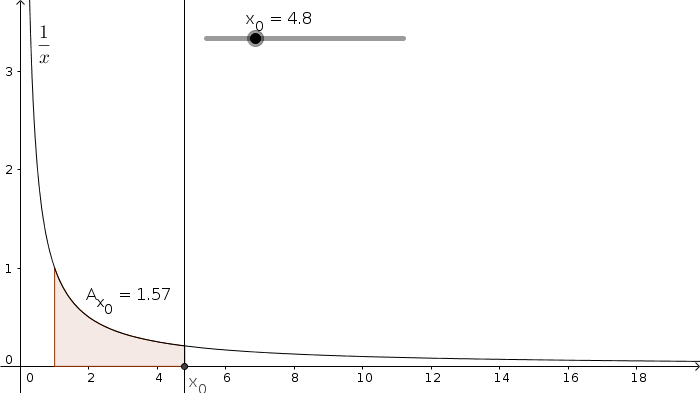
\includegraphics[width=12cm,keepaspectratio=true]{01_ln.png}
\end{center}


\begin{notice}{warning}{Aðvörun:}
Fallið \(\ln\) er bara skilgreint fyrir jákvæðar rauntölur
\end{notice}


\subsection{Setning}
\label{kafli04:setning}
Náttúrlegi logrinn er diffranlegur og afleiðan uppfyllir
\begin{equation*}
\begin{split}\frac{d}{dx}\ln x=\frac{1}{x}.\end{split}
\end{equation*}
Af þessu fylgir að logrinn er samfellt fall.


\subsection{Setning}
\label{kafli04:id1}
Fyrir allar tölur \(x,y>0\) gildir að:
\begin{enumerate}
\item {} 
\(\ln(1) = 0\)

\item {} 
\(\ln(xy)=\ln x+\ln y\)

\item {} 
\(\ln(1/x)=-\ln x\)

\item {} 
\(\ln(x/y)=\ln x-\ln y\)

\item {} 
\(\ln (x^r)=r\ln x\).

\end{enumerate}

\index{veldisvísisfallið}

\section{Veldisvísisfallið}
\label{kafli04:veldisvisisfalli}\label{kafli04:index-1}

\subsection{Setning}
\label{kafli04:id2}
Fallið \(\ln x\) er strangt vaxandi og þar með eintækt.


\subsection{Skilgreining: Veldisvísisfallið}
\label{kafli04:skilgreining-veldisvisisfalli}
\textit{Veldisvísisfallið}, \(\exp x\), er skilgreint sem andhverfa fallsins
\(\ln x\). Skilgreiningarsvæði \(\exp x\) er jafnt myndmengi
\(\ln x\) sem er \({{\mathbb  R}}\). Myndmengi \(\exp x\) er
jafnt skilgreiningarsvæði \(\ln x\) sem er bilið \((0,\infty)\).

\noindent{\hspace*{\fill}\sphinxincludegraphics[width=12cm]{{02_ln-exp}.png}\hspace*{\fill}}

\index{e}\index{veldisvísisfallið!e}

\subsection{Skilgreining: Talan \protect\(e\protect\)}
\label{kafli04:index-2}\label{kafli04:skilgreining-talan}
Skilgreinum töluna með \(e=\exp 1\).

Það þýðir að \(\ln(e)=1\), og talan \(e\) ákvarðast þess vegna
af því að flatarmál svæðisins milli \(x\)-ás og grafs
\(\frac 1x\) á bilinu \([1,e]\) sé 1.

\noindent{\hspace*{\fill}\sphinxincludegraphics[width=12cm]{{02_ln-e}.png}\hspace*{\fill}}

\begin{notice}{note}{Athugasemd:}
\textbf{Hver er munurinn á} \(e^x\) \textbf{og} \(\exp(x)\) \textbf{?}

\(e^x\) er aðeins skilgreint þegar \(x\) er ræð tala, en
\(\exp(x)\) er skilgreint fyrir allar rauntölur því logrinn,
\(\ln:(0,\infty)\to {{\mathbb  R}}\), er átækur.

Það er hins vegar hægt að sýna að
\begin{equation*}
\begin{split}\exp(x)=\lim_{r\to x, r\text{ ræð tala}} e^r.\end{split}
\end{equation*}
Því er eðlilegt að rita fyrir rauntölu \(x\), hvort sem hún er ræð
eða óræð, að \(e^x=\exp x\). Þannig að héðan í frá gerum við engan
greinarmun á \(e^x\) og \(\exp x\), við notum bara það sem lítur
betur út fagurfræðilega.
\end{notice}

\begin{notice}{note}{Athugasemd:}
Athugið að
\begin{equation*}
\begin{split}e^{\ln x}=x \mbox{ fyrir allar tölur }x>0\qquad \mbox{og}
\qquad \ln(e^x)=x  \mbox{ fyrir allar tölur }x.\end{split}
\end{equation*}\end{notice}


\subsection{Eiginleikar veldisvísisfallsins}
\label{kafli04:eiginleikar-veldisvisisfallsins}
Út frá eiginleikum lograns fáum við svo eftirfarandi
\begin{enumerate}
\item {} 
\(e^0=1\)

\item {} 
\(e^{x+y}=e^x e^y\)

\item {} 
\(e^{-x}=\frac{1}{e^x}\)

\item {} 
\(e^{x-y}=\frac{e^x}{e^y}\)

\item {} 
\(\left(e^x\right)^y=e^{xy}\)

\end{enumerate}

\begin{notice}{note}{Athugasemd:}
\textbf{Hænan eða eggið?} Hér höfum við nálgast \(\ln\) og \(\exp\)
þannig að við byrjum á að skilgreina \(\ln\) með heildi (flatarmáli)
og finnum svo andhverfu lograns, \(\exp\).

Einnig væri mögulegt að byrja á því að sýna að \(e^x\) sé vel
skilgreint, ekki bara fyrir ræð \(x\) heldur einnig óræð. Það myndum
við gera með því að nota markgildið
\(\exp(x)=\lim_{r\to x, r\text{ ræð tala}} e^r\)
hér að ofan, og taka þá \(e^x\) sem
skilgreiningu á \(\exp x\) og finna svo andhverfuna, \(\ln\).

Báðar þessar aðferðir hafa kosti og galla, en við notum þá fyrri vegna
þess að hún gefur myndræna framsetningu á logranum.
\end{notice}


\section{Önnur veldisvísisföll og lograr}
\label{kafli04:onnur-veldisvisisfoll-og-lograr}
\index{veldisvísisfallið!grunntala}

\subsection{Skilgreining}
\label{kafli04:skilgreining}\label{kafli04:index-3}
Fyrir tölu \(a>0\) og rauntölu \(x\) skilgreinum við
\begin{equation*}
\begin{split}a^x=e^{x\ln a}.\end{split}
\end{equation*}
\index{logri!grunntala}

\subsection{Skilgreining}
\label{kafli04:id3}\label{kafli04:index-4}
Andhverfa fallsins \(a^x\) er kölluð \emph{logri með grunntölu} \(a\)
og táknuð með \(\log_a x\). Fallið \(\log_a x\) er skilgreint
fyrir öll \(x>0\).


\subsection{Athugasemd}
\label{kafli04:athugasemd}\begin{equation*}
\begin{split}y =\log_a(x)\qquad \text{ þá og því aðeins að } \qquad x = a^y.\end{split}
\end{equation*}

\subsection{Setning}
\label{kafli04:id4}
Fyrir rauntölu \(a>0\) og allar rauntölur \(x,y\) gildir að:
\begin{enumerate}
\item {} 
\(a^0=1\)

\item {} 
\(a^1=a\)

\item {} 
\(a^{x+y}=a^xa^y\)

\item {} 
\(a^{-x}=\frac{1}{a^x}\)

\item {} 
\(a^{x-y}=\frac{a^x}{a^y}\)

\item {} 
\(\big(a^x\big)^y=a^{xy}\)

\item {} 
\((ab)^x=a^xb^x\) (hér er forsenda að \(b>0\)).

\end{enumerate}

Fyrir rauntölu \(a>0\) og allar rauntölur \(x,y\) gildir að:
\begin{enumerate}
\item {} 
\(\log_a 1=0\)

\item {} 
\(\log_a a = 1\)

\item {} 
\(\log_a(xy)=\log_a x+\log_a y\)

\item {} 
\(\log_a (1/x)=-\log_a x\)

\item {} 
\(\log_a (x/y)=\log_a x-\log_a y\)

\item {} 
\(\log_a (x^y)=y\log_a x\)

\item {} 
\(\log_a x=\frac{\log_b x}{\log_b a}\) (hér er forsenda að
\(b>0\)).

\end{enumerate}


\section{Eiginleikar veldisvísisfalla og logra}
\label{kafli04:eiginleikar-veldisvisisfalla-og-logra}

\subsection{Setning}
\label{kafli04:id5}\begin{enumerate}
\item {} 
\(\frac{d}{dx}\ln x=\frac 1x\)

\item {} 
\(\frac{d}{dx}e^x=e^x\)

\item {} 
\(\frac{d}{dx}a^x=(\ln a)a^x\)

\item {} 
\(\frac{d}{dx}\log_a x=\frac{1}{(\ln a)x}\)

\end{enumerate}


\subsection{Setning}
\label{kafli04:id6}
Ef \(a>0\) þá er
\begin{enumerate}
\item {} 
\(\lim_{x\to \infty} \frac{x^a}{e^x} = 0\)

\item {} 
\(\lim_{x\to \infty} \frac{\ln(x)}{x^a} = 0\)

\item {} 
\(\lim_{x\to -\infty} |x|^a e^x = 0\)

\item {} 
\(\lim_{x\to 0^+} x^a\, \ln(x) = 0\)

\end{enumerate}

\begin{notice}{note}{Athugasemd:}
Athugið að setningin að ofan gildir óháð því hversu stórt \(a\) er
(liðir 1 og 3) eða hversu lítið \(a\) er (liðir 2 og 4).

Með öðrum orðum:
\begin{itemize}
\item {} 
Þegar veldi og veldisvísisfall kljást, þá vinnur veldisvísisfallið.

\item {} 
Þegar veldi og logri kljást, þá vinnur veldið.

\end{itemize}
\end{notice}


\section{Andhverfur hornafalla}
\label{kafli04:andhverfur-hornafalla}

\subsection{Andhverfa sínus}
\label{kafli04:andhverfa-sinus}
Fallið \(\sin(x)\) skilgreint á öllum rauntalnaásnum er ekki eintækt
og á sér því ekki andhverfu.

Við getum hins vegar takmarkað okkur við hálfa lotu, þ.e. skoðum bara
\(x\in [-\frac \pi 2, \frac \pi 2]\). \(\sin(x)\) takmarkað við
þetta bil táknum við með \({{\text{Sin}}}(x)\).
\({{\text{Sin}}}\) er strangt vaxandi og því eintækt á þessu bili,
og hefur þar af leiðandi andhverfu.


\subsection{Skilgreining: arcsin}
\label{kafli04:skilgreining-arcsin}
\emph{Andhverfa sínussins}, táknuð \(\arcsin(x)\) (eða
\(\sin^{-1}(x)\)), er andhverfa \({{\text{Sin}}}\) og hefur því
myndmengið \([-\frac \pi 2,
\frac \pi 2]\) og skilgreiningarmengið \([-1,1]\).

\noindent{\hspace*{\fill}\sphinxincludegraphics[width=12cm]{{05_arcsin}.png}\hspace*{\fill}}


\subsection{Andhverfa kósínus}
\label{kafli04:andhverfa-kosinus}
Fallið \(\cos(x)\) skilgreint á öllum rauntalnaásnum er ekki eintækt
og á sér því ekki andhverfu.

Við getum hins vegar takmarkað okkur við hálfa lotu, þ.e. skoðum bara
\(x\in [0, \pi]\). \(\cos(x)\) takmarkað við þetta bil táknum
við með \({{\text{Cos}}}(x)\). \({{\text{Cos}}}\) er strangt
minnkandi og því eintækt á þessu bili, og hefur þar af leiðandi
andhverfu.


\subsection{Skilgreining: arccos}
\label{kafli04:skilgreining-arccos}
\emph{Andhverfa kósínussins}, táknuð \(\arccos(x)\) (eða
\(\cos^{-1}(x)\)), er andhverfa \({{\text{Cos}}}\) og hefur því
myndmengið \([0,\pi]\) og skilgreiningarmengið \([-1,1]\).

\noindent{\hspace*{\fill}\sphinxincludegraphics[width=12cm]{{05_arccos}.png}\hspace*{\fill}}


\subsection{Andhverfa tangens}
\label{kafli04:andhverfa-tangens}
Fallið \(\tan(x) = \frac{\sin(x)}{\cos(x)}\) skilgreint á
\(\{x \in {{\mathbb  R}}; x \neq \pi k + \frac \pi 2, k \in {{\mathbb Z}}\}\)
er ekki eintækt og á sér því ekki andhverfu.

Við getum hins vegar takmarkað okkur við eina lotu, þ.e. skoðum bara
\(x\in (-\frac \pi 2, \frac \pi 2)\). Athugið að hér eru endapunktar
bilsins ekki með. \(\tan(x)\) takmarkað við þetta bil táknum við með
\({{\text{Tan}}}(x)\). \({{\text{Tan}}}\) er strangt vaxandi og
því eintækt á þessu bili, og hefur þar af leiðandi andhverfu.


\subsection{Skilgreining: arctan}
\label{kafli04:skilgreining-arctan}
\emph{Andhverfa tangensins}, táknuð \(\arctan(x)\) (eða
\(\tan^{-1}(x)\)), er andhverfa \({{\text{Tan}}}\) og hefur því
myndmengið \((-\frac \pi 2,
\frac \pi 2)\) og skilgreiningarmengið \((-\infty,\infty)\). Þar að
auki þá er
\(\lim_{x\to \infty} \arctan(x) = \frac \pi 2\) og
\(\lim_{x\to -\infty} \arctan(x) = -\frac \pi 2\).

\noindent{\hspace*{\fill}\sphinxincludegraphics[width=12cm]{{05_arctan}.png}\hspace*{\fill}}


\subsection{Setning}
\label{kafli04:id7}\begin{enumerate}
\item {} 
\(\frac d{dx} \arcsin(x) = \frac 1{\sqrt{1-x^2}}\)

\item {} 
\(\frac d{dx} \arccos(x) = \frac {-1}{\sqrt{1-x^2}}\)

\item {} 
\(\frac d{dx} \arctan(x) = \frac 1{1+x^2}\)

\end{enumerate}


\section{Breiðbogaföll}
\label{kafli04:breibogafoll}

\subsection{Skilgreining: cosh og sinh}
\label{kafli04:skilgreining-cosh-og-sinh}
Við skilgreinum \textit{breiðbogasínus}, \(\sinh\), og \textit{breiðbogakósínus},
\(\cosh\), með eftirfarandi formúlum
\begin{equation*}
\begin{split}\begin{aligned}
\sinh(x) &= \frac{e^x - e^{-x}}2,\\
\cosh(x) &= \frac{e^x + e^{-x}}2.\end{aligned}\end{split}
\end{equation*}
\noindent{\hspace*{\fill}\sphinxincludegraphics[width=12cm]{{06_sinh-cosh}.png}\hspace*{\fill}}


\subsection{Setning}
\label{kafli04:id8}\begin{enumerate}
\item {} 
\(\frac d{dx} \sinh(x) = \cosh(x)\)

\item {} 
\(\frac d{dx} \cosh(x) = \sinh(x)\)

\end{enumerate}

\begin{notice}{warning}{Aðvörun:}
Það er enginn mínus í afleiðu \(\cosh\) eins og í afleiðu \(\cos\).
\end{notice}


\subsection{Setning}
\label{kafli04:id9}\begin{enumerate}
\item {} 
\(\sinh(0) = 0\) og \(\cosh(0) = 1\)

\item {} 
\(\cosh^2(x) - \sinh^2(x) = 1\)

\item {} 
\(\sinh(-x) = -\sinh(x)\)

\item {} 
\(\cosh(-x) = \cosh(x)\)

\item {} 
\(\sinh(x+y) = \sinh(x)\cosh(y) + \cosh(x)\sinh(y)\)

\item {} 
\(\cosh(x+y) = \cosh(x)\cosh(y) + \sinh(x)\sinh(y)\)

\item {} 
\(\cosh(2x) = \cosh^2(x) + \sinh^2(x) = 1+2\sinh^2(x) = 2\cosh^2(x)-1\)

\item {} 
\(\sinh(2x) = 2\sinh(x)\cosh(x)\)

\end{enumerate}


\subsection{Skilgreining: tanh}
\label{kafli04:skilgreining-tanh}
Við skilgreinum \textit{breiðbogatangens} með
\begin{equation*}
\begin{split}\tanh(x) = \frac{\sinh(x)}{\cosh(x)}\end{split}
\end{equation*}

\subsection{Setning}
\label{kafli04:id10}\begin{enumerate}
\item {} 
\(\tanh(x) = \frac{e^x-e^{-x}}{e^x+e^{-x}}\)

\item {} 
\(\frac d{dx} \tanh(x) = \frac{1}{\cosh^2(x)}\)

\item {} 
\(\lim_{x\to \infty} \tanh(x) = 1\)

\item {} 
\(\lim_{x\to -\infty} \tanh(x) = -1\)

\end{enumerate}


\section{Andhverfur breiðbogafalla}
\label{kafli04:andhverfur-breibogafalla}

\subsection{Andhverfa breiðbogasínussins og breiðbogatangensins}
\label{kafli04:andhverfa-breibogasinussins-og-breibogatangensins}
Af Setningum 4.6.1 (2) og 4.6.5 (2) sjáum við að afleiður \(\sinh\) og
\(\tanh\) eru jákvæðar og föllin því stranglega vaxandi. Þau eru þar
með eintæk og eiga sér andhverfur.


\subsection{Skilgreining}
\label{kafli04:id11}
\textit{Andhverfa breiðbogasínussins},
táknuð \({{\text{arsinh}}}(x)\) (eða
\(\sinh^{-1}(x)\)), er andhverfa \(\sinh\) og hefur myndmengið
\((-\infty,\infty)\) og skilgreiningarmengið
\((-\infty,\infty)\). Þar að auki þá er
\begin{equation*}
\begin{split}{{\text{arsinh}}}(x) = \ln\left(x+\sqrt{x^2+1}\right)\end{split}
\end{equation*}
\textit{Andhverfa breiðbogatangensins},
táknuð \({{\text{artanh}}}(x)\)
(eða \(\tanh^{-1}(x)\)), er andhverfa \(\tanh\) og hefur
myndmengið \((-\infty,\infty)\) og skilgreiningarmengið
\((-1,1)\). Þar að auki þá er
\begin{equation*}
\begin{split}{{\text{artanh}}}(x) = \frac 12 \ln\left(\frac{1+x}{1-x}\right)\end{split}
\end{equation*}

\subsection{Andhverfa breiðbogakósínussins}
\label{kafli04:andhverfa-breibogakosinussins}\label{kafli04:index-6}
Þar sem \(\cosh\) er ekki eintækt fall þá verðum við að beita
svipuðum aðferðum eins og þegar við fundum \(\arcsin\) til þess að
finna andhverfu þess.
Það er, við þurfum að takmarka skilgreiningarmengi
þess.

Táknum \(\cosh(x)\) takmarkað við bilið \([0,\infty)\) með
\({{\text{Cosh}}}(x)\). Fallið \({{\text{Cosh}}}\) er strangt
vaxandi og því eintækt á þessu bili, og á sér þar með andhverfu.


\subsection{Skilgreining}
\label{kafli04:id12}
\textit{Andhverfa breiðbogakósínussins}, táknuð \({{\text{arcosh}}}(x)\)
(eða \(\cosh^{-1}(x)\)), er andhverfa \({{\text{Cosh}}}\) og
hefur því myndmengið \([0,\infty)\) og skilgreiningarmengið
\([1,\infty)\). Þar að auki þá er
\begin{equation*}
\begin{split}{{\text{arcosh}}}(x) = \ln\left(x+\sqrt{x^2-1}\right)\end{split}
\end{equation*}
\noindent{\hspace*{\fill}\sphinxincludegraphics[width=12cm]{{07_arcosh}.png}\hspace*{\fill}}


\subsection{Í framtíðinni}
\label{kafli04:i-framtiinni}
Við höfum séð að veldisvísisfallið og logrinn tengjast breiðbogaföllunum
töluvert og það sama á við um hornaföllin. Seinna, nánar tiltekið í
Stærðfræðigreiningu III, þá sjáið þið að hornaföllin og breiðbogaföllin
eru bara mismunandi hliðar á veldisvísisfallinu.

\noindent{\hspace*{\fill}\sphinxincludegraphics[width=10cm]{{07_exp}.png}\hspace*{\fill}}


\chapter{Könnun falla}
\label{kafli05:konnun-falla}\label{kafli05::doc}
\begin{notice}{note}{Athugasemd:}
\textbf{Nauðsynleg undirstaða}
\begin{itemize}
\item {} 
{\hyperref[kafli03:vaxandiminnkandi]{\sphinxcrossref{\DUrole{std,std-ref}{vaxandi/minnkandi föll}}}}

\item {} 
{\hyperref[kafli03:afleidur]{\sphinxcrossref{\DUrole{std,std-ref}{afleiður}}}}

\item {} 
{\hyperref[kafli03:utgildi]{\sphinxcrossref{\DUrole{std,std-ref}{útgildi}}}}

\item {} 
ójöfnur

\end{itemize}
\end{notice}

\emph{``The Guide says there is an art to flying'', said Ford, ``or rather a knack.
The knack lies in learning how to throw yourself at the ground and miss.''}

- Douglas Adams, Life, the Universe and Everything


\bigskip\hrule{}\bigskip



\section{Inngangur}
\label{kafli05:inngangur}
\begin{notice}{warning}{Aðvörun:}
\textbf{Frávik frá bókinni}

Það sem á eftir kemur er eitt af fáum atriðum þar sem mín nálgun og
skilgreiningar eru frábrugðnar þeim í kennslubókinni eftir Adams.
\end{notice}


\subsection{Hver er munurinn?}
\label{kafli05:hver-er-munurinn}
\noindent\begin{tabulary}{\linewidth}{|L|L|}
\hline
\phantomsection\label{kafli05:figa}
\noindent{\hspace*{\fill}\sphinxincludegraphics[width=0.950\linewidth]{{01_f1}.png}\hspace*{\fill}}
&\phantomsection\label{kafli05:figb}
\noindent{\hspace*{\fill}\sphinxincludegraphics[width=0.950\linewidth]{{01_g1}.png}\hspace*{\fill}}
\\
\hline\end{tabulary}


Skoðum föllin tvö að ofan, þau eru augljóslega ekki eins, þannig að
spurningin er hvernig getum við lýst muninum á þeim?

Þau hugtök sem við höfum skoðað hingað til geta ekki greint á milli
þessara falla:
\begin{enumerate}
\item {} 
Þau hafa sama skilgreiningarmengið \([A,B]\)

\item {} 
Þau taka sömu gildin í endapunktunum

\item {} 
Þau hafa bæði hágildi í \(A\) og lággildi í \(B\)

\item {} 
Þau eru bæði samfelld og diffranleg

\item {} 
Þau eru bæði minnkandi (neikvæð afleiða)

\end{enumerate}


\subsection{Drögum sniðil}
\label{kafli05:drogum-sniil}
\noindent\begin{tabulary}{\linewidth}{|L|L|}
\hline
\phantomsection\label{kafli05:figa2}
\noindent{\hspace*{\fill}\sphinxincludegraphics[width=0.950\linewidth]{{01_f2}.png}\hspace*{\fill}}
&\phantomsection\label{kafli05:figb2}
\noindent{\hspace*{\fill}\sphinxincludegraphics[width=0.950\linewidth]{{01_g2}.png}\hspace*{\fill}}
\\
\hline\end{tabulary}


Ef við veljum nú tvo punkta á \([A,B]\) af handahófi, köllum þá
\(x_1\) og \(x_2\), og drögum línu (sniðil) í gegnum punktana á
gröfum \(f\) og \(g\) þá sjáum við að sniðillinn lendir fyrir
neðan \(g\) en ofan \(f\).

Athugum nú að sérhvern punkt á milli \(x_1\) og \(x_2\) getum við skrifað á
forminu
\(\alpha x_1 + (1-\alpha)x_2\), þar sem \(\alpha \in [0,1]\). En \(\alpha=0\)
gefur \(x_2\) og \(\alpha=1\) gefur \(x_1\).

Þá er
\(y\)-hnit punktsins á sniðlinum með þetta \(x\)-hnit gefið með
\begin{equation*}
\begin{split}\alpha f(x_1) + (1-\alpha) f(x_2), \qquad \alpha \in [0,1],\end{split}
\end{equation*}
á fyrri myndinni og
\begin{equation*}
\begin{split}\alpha g(x_1) + (1-\alpha) g(x_2), \qquad \alpha \in [0,1],\end{split}
\end{equation*}
á myndinni fyrir \(g\).

Ef graf \(f\) liggur fyrir neðan sniðilinn þá þýðir það að fallgildi
\(f\) í punktunum \(\alpha x_1 + (1-\alpha)x_2\) liggur fyrir
neðan punktinum á sniðlinum, það er
\begin{equation*}
\begin{split}f(\alpha x_1+(1-\alpha)x_2)\leq \alpha f(x_1)+(1-\alpha)f(x_2).\end{split}
\end{equation*}
Eins, ef graf \(g\) liggur fyrir ofan sniðilinn þá gildir að
\begin{equation*}
\begin{split}g(\alpha x_1+(1-\alpha)x_2)\geq \alpha g(x_1)+(1-\alpha)g(x_2).\end{split}
\end{equation*}
\noindent\begin{tabulary}{\linewidth}{|L|L|}
\hline
\phantomsection\label{kafli05:figa3}
\noindent{\hspace*{\fill}\sphinxincludegraphics[width=0.950\linewidth]{{01_f3}.png}\hspace*{\fill}}
&\phantomsection\label{kafli05:figb3}
\noindent{\hspace*{\fill}\sphinxincludegraphics[width=0.950\linewidth]{{01_g3}.png}\hspace*{\fill}}
\\
\hline\end{tabulary}



%\begin{center}
%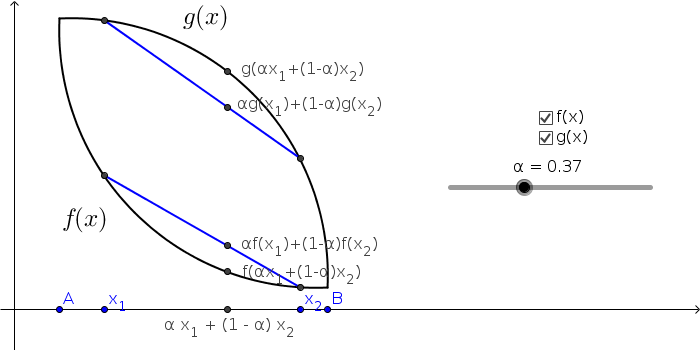
\includegraphics[width=12cm,keepaspectratio=true]{01_kupni.png}
%\end{center}



\bigskip\hrule{}\bigskip



\section{Kúpni}
\label{kafli05:kupni}
\index{kúpni}\index{fall!kúpt}\index{fall!hvelft}

\subsection{Skilgreining: Kúpt/hvelft}
\label{kafli05:index-0}\label{kafli05:skilgreining-kupt-hvelft}
Látum \(f:[a, b]\rightarrow {\mathbb  R}\) vera fall.
\begin{enumerate}
\item {} 
Segjum að fallið \(f\) sé \textit{kúpt} ef um
alla punkta \(x_1, x_2\in [a, b]\) og sérhverja tölu
\(0\leq
\alpha\leq 1\) gildir að
\begin{equation*}
\begin{split}f(\alpha x_1+(1-\alpha)x_2)\leq \alpha f(x_1)+(1-\alpha)f(x_2).\end{split}
\end{equation*}
\item {} 
Segjum að fallið \(f\) sé \textit{hvelft}
ef um alla punkta \(x_1, x_2\in [a, b]\) og sérhverja tölu
\(0\leq
\alpha\leq 1\) gildir að
\begin{equation*}
\begin{split}f(\alpha x_1+(1-\alpha)x_2)\geq \alpha f(x_1)+(1-\alpha)f(x_2).\end{split}
\end{equation*}
\end{enumerate}

\begin{notice}{note}{Athugasemd:}
Hér erum við komin með hugtak sem getur útskýrt muninn á myndunum í byrjun
kaflans, \(f\) er kúpt og \(g\) er hvelft.
\end{notice}


\bigskip\hrule{}\bigskip



\section{Auðkenning á kúpni með afleiðum}
\label{kafli05:aukenning-a-kupni-me-afleium}
\noindent\begin{tabulary}{\linewidth}{|L|L|}
\hline
\phantomsection\label{kafli05:id1}
\noindent{\hspace*{\fill}\sphinxincludegraphics[width=0.950\linewidth]{{01_f1}.png}\hspace*{\fill}}
&\phantomsection\label{kafli05:id2}
\noindent{\hspace*{\fill}\sphinxincludegraphics[width=0.950\linewidth]{{01_g1}.png}\hspace*{\fill}}
\\
\hline\end{tabulary}



\subsection{Athugasemd}
\label{kafli05:athugasemd}
Ef við skoðum afleiður fallanna \(f\) og \(g\) betur þá sjáum
við að:
\begin{enumerate}
\item {} 
Afleiða \(f\) er mjög neikvæð nálægt \(A\) og nálgast svo 0
í \(B\), það er afleiðan er vaxandi.

\item {} 
Afleiða \(g\) er u.þ.b. 0 í \(A\) og minnkar svo þegar við
nálgumst \(B\), það er afleiðan er minnkandi.

\end{enumerate}

Með öðrum orðum
\begin{equation*}
\begin{split}(f')' = f'' \geq 0 \qquad   \text{og} \qquad
    (g')' = g'' \leq 0.\end{split}
\end{equation*}

\subsection{Setning}
\label{kafli05:setning}
Fyrir tvídiffranlegt fall \(f\) þá er eftirfarandi jafngilt
\begin{enumerate}
\item {} 
\(f\) er kúpt

\item {} 
\(f'\) er vaxandi

\item {} 
\(f'' \geq 0\)

\end{enumerate}


\subsection{Setning}
\label{kafli05:id3}\label{kafli05:index-1}
Fyrir tvídiffranlegt fall \(g\) þá er eftirfarandi jafngilt
\begin{enumerate}
\item {} 
\(g\) er hvelft

\item {} 
\(g'\) er minnkandi

\item {} 
\(g'' \leq 0\)

\end{enumerate}

\begin{notice}{warning}{Aðvörun:}
Hvort fall er kúpt eða hvelft er \textbf{algjörlega óháð} því hvort það er
vaxandi eða minnkandi. Til dæmis er \(f(x) = x^2\) kúpt en það er
vaxandi þegar \(x>0\) og minnkandi þegar \(x<0\).
\end{notice}

\begin{notice}{warning}{Aðvörun:}
Föll eru ekki alltaf annað hvort kúpt eða hvelft alls staðar. Alveg
eins og það eru til föll sem eru sums staðar vaxandi og sums staðar
minnkandi, þá eru mörg föll sums staðar kúpt og sums staðar hveld.
Þetta á til dæmis við um hornaföllin.
\end{notice}


\bigskip\hrule{}\bigskip



\section{Beygjuskilapunktar}
\label{kafli05:beygjuskilapunktar}
\index{beygjuskilapunktar}

\subsection{Skilgreining}
\label{kafli05:index-2}\label{kafli05:skilgreining}
Punktur \((x_0, f(x_0))\) er sagður vera \textit{beygjuskilapunktur}
grafsins \(y=f(x)\) ef
\begin{enumerate}
\item {} 
grafið hefur snertilínu í \(x_0\), og

\item {} 
grafið er kúpt öðru megin við \(x_0\) og hvelft hinum megin við
\(x_0\).

\end{enumerate}


\subsection{Setning}
\label{kafli05:id4}
Ef fallið \(f\) er tvídiffranlegt þá er punkturinn \(x_0\)
beygjuskilapunktur fallsins \(f\) ef og aðeins ef
\(f''(x_0) =0\) og \(f''\) skiptir um formerki í \(x_0\).

\noindent{\hspace*{\fill}\sphinxincludegraphics[width=12cm]{{04_beygjuskilapunktur}.png}\hspace*{\fill}}

\index{útgildi!út frá annarri afleiðu}

\section{Útgildi}
\label{kafli05:utgildi}\label{kafli05:index-3}

\subsection{Hvar á að leita útgilda}
\label{kafli05:hvar-a-a-leita-utgilda}
{\hyperref[kafli03:utgildi]{\sphinxcrossref{\DUrole{std,std-ref}{Útgildi}}}}  skoðuðum við í kafla 3.5, en nú ætlum við að skoða
hvernig önnur afleiðan nýtist til að finna og flokka útgildi.

Punktar sem koma til greina fyrir staðbundin útgildi falls \(f\) eru
\begin{enumerate}
\item {} 
punktar \(x_0\) þar sem \(f'(x_0)=0\),

\item {} 
punktar \(x_0\) þar sem \(f'(x_0)\) er ekki skilgreint,

\item {} 
þeir endapunktar skilgreiningarmengisins þar sem fallið er
skilgreint.

\end{enumerate}


\subsection{Hágildi/lágildi út frá formerki afleiðu}
\label{kafli05:hagildi-lagildi-ut-fra-formerki-afleiu}
Látum \(x_0\) vera innri punkt á skilgreiningarsvæði \(f\).
Gerum ráð fyrir að \(f\) sé diffranlegt í öllum punktum í einhverju
bili utan um \(x_0\) og að \(f'(x_0)=0\).
\begin{enumerate}
\item {} 
Ef formerki \(f'\) breytist úr plús í mínus í \(x_0\)
(farið frá vinstri til hægri eftir rauntalnaásnum) þá er
staðbundið hágildi í \(x_0\).

\item {} 
Ef formerki \(f'\) breytist úr mínus í plús í \(x_0\) þá
er staðbundið lággildi í \(x_0\).

\item {} 
Ef formerki \(f'\) breytist ekki í \(x_0\) þá er hvorki
há- né lággildi í \(x_0\).

\end{enumerate}


\subsection{Útgildi og önnur afleiðan}
\label{kafli05:utgildi-og-onnur-afleian}\begin{enumerate}
\item {} 
Ef \(f'(x_0)=0\) og \(f''(x_0)<0\) þá er \(x_0\)
staðbundið hágildi.

\item {} 
Ef \(f'(x_0)=0\) og \(f''(x_0)>0\) þá er \(x_0\)
staðbundið lággildi.

\end{enumerate}

\begin{notice}{warning}{Aðvörun:}
Athugið að ef \(f''(x_0)=0\) þá getur \(x_0\) verið hvort sem er
staðbundið hágildi, staðbundið lággildi eða beygjuskilapunktur.
\end{notice}

\index{aðfellur}\index{aðfellur!lóðrétt}\index{aðfellur!lárétt}\index{aðfellur!skáfella}\index{skáfella|see{aðfellur}}

\section{Aðfellur}
\label{kafli05:afellur}\label{kafli05:index-4}

\subsection{Skilgreining: Lóðrétt aðfella}
\label{kafli05:skilgreining-lorett-afella}
Fallið \(f\) hefur \emph{lóðrétta aðfellu} í punktinum \(a\) ef
\(\lim_{x\to a^-} f(x) = \pm \infty\) og/eða
\(\lim_{x\to a^+} f(x) = \pm \infty\).
\begin{quote}

Aðfellan er þá línan \(x=a\).
\end{quote}

\noindent{\hspace*{\fill}\sphinxincludegraphics[width=12cm]{{06_lodfellur}.png}\hspace*{\fill}}

\emph{Fallið} \(\frac{1}{\sin(x)}\) \emph{hefur lóðréttar aðfellur í öllum punktum þar sem} \(\sin(x)=0\).


\subsection{Skilgreining: Lárétt aðfella}
\label{kafli05:skilgreining-larett-afella}
Fallið \(f\) hefur \emph{lárétta aðfellu} ef
\(\lim_{x\to \infty} f(x) = L\) og/eða
\(\lim_{x\to -\infty} f(x) = L\).

Aðfellan er þá línan \(y=L\).

\noindent{\hspace*{\fill}\sphinxincludegraphics[width=12cm]{{06_arctanadfellur}.png}\hspace*{\fill}}

\emph{Fallið} \(\arctan(x)\) \emph{hefur tvær láréttar aðfellur,} \(y=\frac{\pi}{2}\) \emph{og} \(y=\frac{-\pi}{2}\).


\subsection{Skáfella}
\label{kafli05:skafella}
Fallið \(f\) hefur \emph{skáfellu} ef til eru \(a\) og \(b\)
þannig að \(\lim_{x\to \infty} f(x) -ax-b = 0\) og/eða
\(\lim_{x\to -\infty} f(x) -ax-b= 0\).

Skáfellan er þá línan \(y=ax+b\).

\noindent{\hspace*{\fill}\sphinxincludegraphics[width=12cm]{{06_lodogskafellur}.png}\hspace*{\fill}}

\emph{Fallið} \(\frac{x^2}{2x-4}\) \emph{hefur skáfelluna} \(y=\frac{1}{2}x+1\) \emph{auk lóðréttu aðfellunnar} \(x=2\).


\bigskip\hrule{}\bigskip

\newpage

\section{Að teikna graf falls}
\label{kafli05:a-teikna-graf-falls}
Þegar teikna á graf fallsins \(f\) er gagnlegt að fara í gegnum atriðin á eftirfarandi lista:
\begin{enumerate}
\item {} 
Ákvarðið \(f'\) og \(f''\) og þáttið útkomurnar ef hægt er.

\item {} \begin{description}
\item[{Kannið \(f\) til að ákvarða skilgreiningarmengi þess auk eftirfarandi eiginleika:}] \leavevmode\begin{enumerate}
\item {} 
Lóðréttar aðfellur. (Leitið að rótum nefnara)

\item {} 
Láréttar aðfellur og skáfellur. (Finnið \(\lim_{x \to \pm\infty}f(x)\).)

\item {} 
Samhverfa (er \(f\) jafnstætt eða oddstætt?)

\item {} 
Skurðpunktar við ása (punktar með hnit \((x,0)\) eða \((0,y)\)), endapunktar skilgreiningamengisins eða aðrir punktar á grafinu þar sem einfalt er að reikna út bæði hnitin.

\end{enumerate}

\end{description}

\item {} \begin{description}
\item[{Kannið \(f'\) til að ákvarða eftirfarandi:}] \leavevmode\begin{enumerate}
\item {} 
Útgildispunkta.

\item {} 
Punktar þar sem \(f'\) er ekki skilgreint (sérstöðupunktar, endapunktar skilgreiningarmengis \(f\) og lóðréttar aðfellur)

\item {} 
Bilin þar sem \(f'\) er jákvætt
og neikvætt. Það er góð hugmynd að setja þessar upplýsingar fram í töflu. Á töfluna má svo líka merkja inn niðurstöður um hvar \(f\) er vaxandi og minnkandi og hvort útgildispunktar séu staðbundin hágildi eða lággildi.

\end{enumerate}

\end{description}

\item {} \begin{description}
\item[{Kannið \(f''\) til að ákvarða eftirfarandi:}] \leavevmode\begin{enumerate}
\item {} 
Punktar þar sem \(f''(x)=0\).

\item {} 
Punktar þar sem \(f''\) er ekki skilgreint (sérstöðupunktar, endapunktar skilgreiningarmengis \(f\) og lóðréttar aðfellur, e.t.v. auk fleiri punkta þar sem \(f'\) er skilgreint en ekki \(f''\).)

\item {} 
Bilin þar sem \(f''\) er jákvætt og neikvætt og \(f\) þar af leiðandi kúpt og hvelft. Hér er gagnlegt að útbúa töflu.

\item {} 
Beygjuskilapunktar.

\end{enumerate}

\end{description}

\end{enumerate}


\bigskip\hrule{}\bigskip

\newpage
\index{útgildisverkefni}

\section{Útgildisverkefni}
\label{kafli05:utgildisverkefni}\label{kafli05:index-5}

\subsection{Markmiðið}
\label{kafli05:markmii}
Útgildisverkefni snúast um það að hámarka eða lágmarka tiltekna stærð, t.d.
verð, rúmmál, lengd, ... . Þá þarf að finna (helst diffranlegt) fall fyrir stærðina
sem við höfum áhuga á hámarka/lágmarka en þó með þeim skorðum sem vandamálið setur okkur.

Til þess að þetta sé mögulegt má fallið bara vera háð einni breytu og
það þarf helst að vera diffranlegt.

Þá getum við fundið útgildi með þeim aðferðum sem við erum búin að koma
okkur upp.


\subsection{Að leysa útgildisvandamál}
\label{kafli05:a-leysa-utgildisvandamal}
Sjá einnig bls. 260 (8. útg.), 259 (7. útg.) eða 238 (6. útg.) í kennslubókinni.
\begin{enumerate}
\item {} 
Lesið vandamálið vandlega og áttið ykkur á því hvert það er og
hvað á að finna.

\item {} 
Teiknið mynd ef mögulegt er, hún gefur oft upplýsingar um skorður
sem hjálpa okkur að útbúa fallið.

\item {} 
Skilgreinið aukabreytur.

\item {} 
Skilgreinið fallið, sem fall af einni eða fleiri breytum.

\item {} 
Finnið skorður (jöfnur) sem hægt er að stinga inn í fallið

\item {} 
Skrifið fallið sem fall af einni breytu.

\item {} 
Finnið útgildi

\item {} 
Dragið ályktanir af niðurstöðunni, og athugið hvort hún sé
raunhæf miðað við verkefnið (rúmmál á ekki að vera neikvætt og
þess háttar).

\end{enumerate}


\subsection{Dæmi: Gosdós}
\label{kafli05:daemi-gosdos}
Hvert er hagkvæmasta formið á sívalningslaga gosdós?

\noindent{\hspace*{\fill}\sphinxincludegraphics[height=7cm]{{09_cylinder}.png}\hspace*{\fill}}


\subsection{Dæmi: Kassi}
\label{kafli05:daemi-kassi}
Hvernig er stærsti (mesta rúmmálið) loklausi kassinn sem hægt er búa til úr
örk sem er \(12 \times 12\)?

\noindent{\hspace*{\fill}\sphinxincludegraphics[width=12cm]{{09_kassi}.png}\hspace*{\fill}}


\chapter{Heildun}
\label{kafli06:heildun}\label{kafli06::doc}
\begin{notice}{note}{Athugasemd:}
\textbf{Nauðsynleg undirstaða}
\begin{itemize}
\item {} 
markgildi

\item {} 
afleiður

\item {} 
keðjureglan

\item {} 
reiknireglur fyrir afleiður

\end{itemize}
\end{notice}

\emph{It can be very dangerous to see things from somebody else's point of view without the proper training.}

- Douglas Adams, The Ultimate Hitchhiker's Guide : Five Complete Novels and One Story

\index{heildi!jákvæðs falls}\index{heildi}\index{heildismörk}\index{fall!heildanlegt}\index{flatarmál}

\bigskip\hrule{}\bigskip



\section{Heildun}
\label{kafli06:id1}

\subsection{Óformleg skilgreining á heildi jákvæðs falls}
\label{kafli06:oformleg-skilgreining-a-heildi-jakvaes-falls}
Látum \(f:[a,b]\rightarrow {{\mathbb  R}}\) vera fall þannig að
\(f(x)\geq 0\) fyrir öll \(x\in[a,b]\).

Þegar \textit{heildið} \(\int_a^b f(x)\,dx\) er skilgreint er útkoman úr því
flatarmál svæðisins sem liggur á milli \(x\)-ás og grafs fallsins
(og afmarkast til vinstri af línunni \(x=a\) og til hægri af línunni
\(x=b\)).

Ef heildið \(\int_a^b f(x)\,dx\) er skilgreint þá segjum við að
fallið \(f\) sé \textit{heildanlegt} yfir bilið \([a,b]\).

Tölurnar \(a\) og \(b\) kallast \textit{heildismörk} heildisins.


\subsection{Skilgreining}
\label{kafli06:skilgreining}
Látum \(f\) vera fall. Skilgreinum föllin \(f_+\) og
\(f_-\), sem bæði hafa sama skilgreiningarsvæði og \(f\), með
\begin{equation*}
\begin{split}f_+(x)=\left\{\begin{array}{ll} f(x) & \mbox{ef }f(x)\geq 0,\\
  0 & \mbox{ef }f(x)<0, \end{array} \right. \qquad
  f_-(x)=\left\{\begin{array}{ll} 0 & \mbox{ef }f(x)\geq 0,\\
  -f(x) & \mbox{ef }f(x)<0. \end{array}\right.\end{split}
\end{equation*}
Athugið að \(f(x)=f_+(x)-f_-(x)\).

\noindent{\hspace*{\fill}\sphinxincludegraphics[width=12cm]{{01_fplusminus}.png}\hspace*{\fill}}


\subsection{Óformleg skilgreining á heildi falls}
\label{kafli06:oformleg-skilgreining-a-heildi-falls}
Takmarkað fall \(f\) er \emph{heildanlegt} yfir bilið \([a, b]\) ef
bæði föllin \(f_+\) og \(f_-\) eru heildanleg yfir bilið
\([a,
b]\). Ef fallið \(f\) er heildanlegt þá skilgreinum við heildi þess
með formúlunni
\begin{equation*}
\begin{split}\int_a^b f(x)\,dx=\int_a^b f_+(x)\,dx-\int_a^b f_-(x)\,dx.\end{split}
\end{equation*}
\begin{notice}{note}{Athugasemd:}
Flatarmálið sem er undir \(x\)-ás reiknast neikvætt.
\end{notice}


\section{Undir- og yfirsummur}
\label{kafli06:undir-og-yfirsummur}

\subsection{Dæmi: Að finna heildi}
\label{kafli06:daemi-a-finna-heildi}
Hvernig getum við fundið flatarmálið \(\int_a^b f(x)\, dx\)?

\textbf{Svar:} Við þurfum að nálga flatarmálið með formum sem hafa þekkt
flatarmál, til dæmis rétthyrningum.

\index{undirsumma}\index{heildun!undirsumma}

\subsection{Skilgreining: Undirsumma}
\label{kafli06:skilgreining-undirsumma}\label{kafli06:index-1}
Skiptum bilinu \([a,b]\) í \(n\) parta. Á hverjum parti komum
við fyrir rétthyrning sem liggur undir grafi fallsins, þ.e. hæðin á
honum er lággildi fallsins á þessum tiltekna parti.

\noindent{\hspace*{\fill}\sphinxincludegraphics[width=12cm]{{03_undirsumma}.png}\hspace*{\fill}}

Látum \(u_k\) vera flatarmál rétthyrninganna, þar sem
\(k=1,\ldots,n\).

Við köllum flatarmál allra rétthyrninganna \textit{undirsummu} fyrir heildið og
táknum hana með \(U(n)\), það er \(U(n) = \sum_{k=1}^n u_k\).

Þá er augljóslega \(U(n) \leq \int_a^b f(x)\, dx\).

Þegar \(n\) stækkar þá fáum við betri og betri nálgun á heildinu.

\index{yfirsumma}\index{heildun!yfirsumma}

\subsection{Skilgreining: Yfirsumma}
\label{kafli06:skilgreining-yfirsumma}\label{kafli06:index-2}
Skiptum bilinu \([a,b]\) í \(n\) parta. Á hverjum parti komum
við fyrir rétthyrning sem er þannig að hæðin á honum er hágildi fallsins
á þessum tiltekna parti.

\noindent{\hspace*{\fill}\sphinxincludegraphics[width=12cm]{{03_yfirsumma}.png}\hspace*{\fill}}

Táknum flatarmál hans með \(y_k\), þar sem \(k=1,\ldots,n\). Við
köllum summu flatarmáls allra rétthyrninganna \textit{yfirsummu} fyrir heildið
og táknum hana með \(Y(n)\), það er \(Y(n) = \sum_{k=1}^n y_k\).

Þá fæst að \(\int_a^b f(x)\, dx \leq Y(n)\).

Þegar \(n\) stækkar þá fáum við betri og betri nálgun á heildinu.


\subsection{Skilgreining: Heildi}
\label{kafli06:skilgreining-heildi}
Ef til er \textbf{nákvæmlega ein} tala \(I\) þannig að
\begin{equation*}
\begin{split}U(n) \leq I \leq Y(n),\end{split}
\end{equation*}
fyrir allar undirsummur \(U(n)\) og yfirsummur \(Y(n)\) þá er
fallið \(f\) heildanlegt á \([a,b]\) og
\begin{equation*}
\begin{split}I = \int_a^b f(x)\, dx.\end{split}
\end{equation*}

\begin{center}
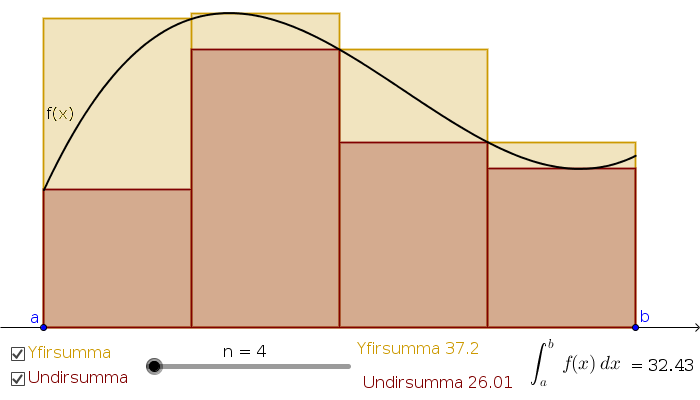
\includegraphics[width=12cm,keepaspectratio=true]{./03_undirogyfirsumma.png}
\end{center}


\begin{notice}{note}{Athugasemd:}
Við sögðum ekkert um það hvernig við skiptum bilinu \([a,b]\) í
\(n\) parta. Það má gera hvernig sem er, það er ekki nauðsynlegt að
þeir séu allir jafn stórir. Eina krafan er að stærð allra parta stefni á
0 þegar \(n\to \infty\).
\end{notice}

\begin{notice}{note}{Athugasemd:}
Við erum ekki bundin af því að skoða rétthyrninga sem með hæð sem er
há/lággildi fallsins á hverjum parti, t.d. má taka miðgildið á hverjum
parti, gildið í hægri endapunkti eða gildið í vinstri endapunkti.

Niðurstaðan þegar \(n\to \infty\) verður hins vegar alltaf sú sama,
þ.e. við nálgumst heildið.
\end{notice}

\begin{notice}{note}{Athugasemd:}
Einnig er mögulegt að nálga heildið með öðrum formum en rétthyrningum,
t.d.trapisum, og hentar það hugsanlega betur í
tölulegum útreikningum.
\end{notice}


\section{Eiginleikar heildisins}
\label{kafli06:eiginleikar-heildisins}

\subsection{Setning}
\label{kafli06:setning}\begin{enumerate}
\item {} 
Ef fallið \(f\) er samfellt á bilinu \([a, b]\) þá er
\(f\) heildanlegt yfir bilið \([a, b]\).

\item {} 
Einhalla fall skilgreint á bili \([a,b]\) er heildanlegt.

\end{enumerate}


\subsection{Setning}
\label{kafli06:id2}
Látum \(f\) vera fall sem er heildanlegt yfir bilið \([a, b]\).
Þá er
\begin{equation*}
\begin{split}\Big|\int_a^b f(x)\,dx\Big|\leq \int_a^b |f(x)|\,dx.\end{split}
\end{equation*}

\subsection{Skilgreining: Heildismörkunum snúið við}
\label{kafli06:skilgreining-heildismorkunum-snui-vi}
Ef fallið \(f\) er heildanlegt yfir bilið \([a,b]\) (hér er
\(a<b\)) þá skilgreinum við
\begin{equation*}
\begin{split}\int_b^a f(x)\,dx=-\int_a^b f(x)\,dx.\end{split}
\end{equation*}

\subsection{Setning}
\label{kafli06:id3}\begin{enumerate}
\item {} 
\(\int_a^a f(x)\,dx=0\).

\item {} 
\(\int_a^b f(x)\,dx=\int_a^c f(x)\,dx+\int_c^b f(x)\,dx\)

(Hér er náttúrlega forsenda að öll heildin séu skilgreind.)

\end{enumerate}


\subsection{Setning}
\label{kafli06:id4}
Látum \(f\) og \(g\) vera föll sem eru heildanleg yfir bilið
\([a,b]\) og látum \(A\) og \(B\) vera fasta. Þá er
\begin{equation*}
\begin{split}\int_a^b Af(x)+Bg(x)\,dx=A\int_a^b f(x)\,dx+B\int_a^b g(x)\,dx.\end{split}
\end{equation*}
Með öðrum orðum, heildun er línuleg aðgerð.


\subsection{Setning}
\label{kafli06:id5}
Látum \(f\) vera fall sem er heildanlegt yfir bilið \([a, b]\).
Gerum ráð fyrir að um öll \(x\in [a, b]\) gildi að
\(f(x)\geq 0\). Þá er
\begin{equation*}
\begin{split}\int_a^b f(x)\,dx\geq 0.\end{split}
\end{equation*}

\subsection{Fylgisetning}
\label{kafli06:fylgisetning}\begin{enumerate}
\item {} 
Látum \(f\) og \(g\) vera föll sem eru heildanleg yfir
bilið \([a, b]\). Gerum ráð fyrir að um öll \(x\in [a, b]\)
gildi að \(f(x)\leq g(x)\). Þá er
\begin{equation*}
\begin{split}\int_a^b f(x)\,dx\leq \int_a^b g(x)\,dx.\end{split}
\end{equation*}
\item {} 
Látum \(f\) vera fall sem er heildanlegt yfir bilið
\([a, b]\). Ef \(m\) og \(M\) eru fastar þannig að um
öll \(x\in [a, b]\) gildir að \(m\leq f(x)\leq M\) þá er
\begin{equation*}
\begin{split}m(b-a)= \int_a^b m\,dx \leq  \int_a^b f(x)\,dx \leq \int_a^b M\,dx =M(b-a).\end{split}
\end{equation*}
\end{enumerate}


\subsection{Setning}
\label{kafli06:id6}
Látum \(f\) vera fall sem er heildanlegt yfir bil \([-a, a]\).
\begin{enumerate}
\item {} 
Ef fallið \(f\) er oddstætt þá er
\begin{equation*}
\begin{split}\int_{-a}^a f(x)\,dx=0.\end{split}
\end{equation*}
\item {} 
Ef fallið \(f\) er jafnstætt þá er
\begin{equation*}
\begin{split}\int_{-a}^a f(x)\,dx=2\int_0^a f(x)\,dx.\end{split}
\end{equation*}
\end{enumerate}

\index{fall!meðalgildi}

\subsection{Skilgreining}
\label{kafli06:id7}\label{kafli06:index-3}
Látum \(f\) vera fall sem er heildanlegt yfir bilið \([a, b]\).
\textit{Meðalgildi} fallsins \(f\) á bilinu \([a, b]\) er skilgreint
sem
\begin{equation*}
\begin{split}\bar{f}=\frac{1}{b-a}\int_{a}^b f(x)\,dx.\end{split}
\end{equation*}
\index{milligildissetning!fyrir heildi}

\subsection{Setning: Meðalgildissetning fyrir heildi}
\label{kafli06:setning-mealgildissetning-fyrir-heildi}\label{kafli06:index-4}
Gerum ráð fyrir að fallið \(f\) sé \textbf{samfellt} á bilinu
\([a, b]\). Þá er til punktur \(c\) í bilinu \([a, b]\)
þannig að
\begin{equation*}
\begin{split}\int_a^b f(x)\,dx=(b-a)f(c).\end{split}
\end{equation*}
Það er að segja, til er punktur \(c\) í bilinu \([a, b]\) þannig
að \(f(c)=\bar{f}\).


\section{Undirstöðusetning stærðfræðigreiningarinnar}
\label{kafli06:undirstousetning-staerfraeigreiningarinnar}
\index{fall!skilgreint með heildi}

\subsection{Skilgreining og setning: Fall skilgreint með heildi}
\label{kafli06:index-5}\label{kafli06:skilgreining-og-setning-fall-skilgreint-me-heildi}
Látum \(f\) vera fall sem er heildanlegt yfir bil \([a, b]\).
Fyrir \(x\in[a, b]\) skilgreinum við \(F(x)=\int_a^x f(t)\,dt\).
Fallið \(F\) er samfellt á \([a, b]\).

\begin{notice}{warning}{Aðvörun:}
Athugið að \(t\) er breytan sem er heildað með tilliti til, en
\(x\) er haldið föstu á meðan. \(t\) hverfur svo þegar búið er
að reikna heildið.
\end{notice}

\index{undirstöðusetning stærðfræðigreiningar}\index{fyrri hluti}

\subsection{Setning: Undirstöðusetning stærðfræðigreiningar, fyrri hluti}
\label{kafli06:undirstodusetning-fyrri}\label{kafli06:index-6}\label{kafli06:setning-undirstousetning-staerfraeigreiningar-fyrri-hluti}
Gerum ráð fyrir að fallið \(f\) sé samfellt á bili \(I\) og
\(a\) sé punktur í \(I\). Fyrir \(x\) í \(I\)
skilgreinum við \(F(x)=\int_a^x f(t)\,dt\). Þá er fallið \(F\)
diffranlegt og
\begin{equation*}
\begin{split}F'(x)=f(x)\end{split}
\end{equation*}
fyrir öll \(x\in I\).

\index{stofnfall}

\section{Stofnföll}
\label{kafli06:stofnfoll}\label{kafli06:index-7}

\subsection{Skilgreining: Stofnfall}
\label{kafli06:skilgreining-stofnfall}
Látum \(f\) vera fall sem er skilgreint á bili \(I\). Fall
\(G\) kallast \textit{stofnfall} fyrir \(f\) á
bilinu \(I\) ef \(G'(x)=f(x)\) fyrir öll \(x\) í \(I\).


\subsection{Fylgisetning}
\label{kafli06:id8}
Látum \(f\) vera samfellt fall skilgreint á bili \(I\). Þá er
til stofnfall fyrir \(f\)
samkvæmt {\hyperref[kafli06:undirstodusetning\string-fyrri]{\sphinxcrossref{\DUrole{std,std-ref}{fyrri hluta undirstöðustöðusetningarinnar}}}}.


\subsection{Hjálparsetning}
\label{kafli06:hjalparsetning}
Ef \(F\) og \(G\) eru hvor tveggja stofnföll fyrir \(f\) á
bilinu \(I\), þá er til fasti \(C\) þannig að
\(F(x)=G(x)+C\) fyrir öll \(x\) í \(I\).

\textbf{Sönnun}: Þar sem
\begin{equation*}
\begin{split}\frac{d}{dx}(G(x) - F(x)) = G'(x) - F'(x) = f(x) - f(x) = 0\end{split}
\end{equation*}
fyrir öll \(x\in I\) þá er \(G(x)-F(x) = C\) fasti.

\index{undirstöðusetning stærðfræðigreiningar}\index{seinni hluti}

\subsection{Setning: Undirstöðusetning stærðfræðigreiningar, seinni hluti}
\label{kafli06:index-8}\label{kafli06:setning-undirstousetning-staerfraeigreiningar-seinni-hluti}
Ef \(f\) er samfellt fall á bilinu \(I\) og \(G\) er
eitthvert stofnfall fyrir \(f\) þá er
\begin{equation*}
\begin{split}\int_a^b f(t)\,dt=G(b)-G(a).\end{split}
\end{equation*}
\begin{notice}{note}{Athugasemd:}
Það skiptir ekki máli hvaða stofnfall er valið í setningunni að ofan,
heildið er alltaf það sama.
\end{notice}


\subsection{Ritháttur}
\label{kafli06:rithattur}
Þegar \(F\) er stofnfall fyrir \(f\) þá ritum við
\begin{equation*}
\begin{split}\int_a^b f(x)\,dx=F(x)\,\bigg|_a^b= F(b)-F(a),\end{split}
\end{equation*}
eða
\begin{equation*}
\begin{split}\int_a^b f(x)\,dx=\left[F(x)\right]_a^b= F(b)-F(a).\end{split}
\end{equation*}

\bigskip\hrule{}\bigskip



\section{Aðferðir við að reikna stofnföll}
\label{kafli06:aferir-vi-a-reikna-stofnfoll}
Skilgreiningin á heildi með undir- og yfirsummum er gagnleg til að útskýra
og sanna eiginleika heilda en hún er ekki mjög góð til þess að reikna
heildi. Því er nauðsynlegt að koma sér upp tólum sem henta betur til þess.
Ef þau duga ekki þá þurfum við að grípa til tölulegra reikninga.


\subsection{Verkfærin}
\label{kafli06:verkfaerin}
Helstu tæknilegu aðferðirnar við að finna stofnföll eru:
\begin{enumerate}
\item {} 
\textit{Innsetning} / breytuskipti.

\item {} 
\textit{Hlutheildun}.

\item {} 
\textit{Stofnbrotaliðun}.

\end{enumerate}


\subsection{Athugasemd}
\label{kafli06:athugasemd}
Gerum ráð fyrir að \(F\) sé stofnfall \(f\), þ.e.
\begin{equation*}
\begin{split}F(x)=\int f(t)\,dt.\end{split}
\end{equation*}
Svo að
\begin{equation*}
\begin{split}F'(x)=f(x).\end{split}
\end{equation*}
Látum nú \(g\) vera fall og skoðum fallið \(F\circ g\). Þá fæst
samkvæmt {\hyperref[kafli03:kedjuregla]{\sphinxcrossref{\DUrole{std,std-ref}{keðjureglunni}}}} að
\begin{equation*}
\begin{split}\frac{d}{dx}F(g(x))=F'(g(x))g'(x) = f(g(x))g'(x),\end{split}
\end{equation*}
eða, með því að heilda beggja vegna jafnaðarmerkisins,
\begin{equation*}
\begin{split}F(g(x))+C = \int f(g(x))g'(x)\,dx.\end{split}
\end{equation*}
\index{heildun!innsetning}

\subsection{Innsetning}
\label{kafli06:index-9}\label{kafli06:innsetning}
Ef við viljum reikna \(\int f(g(x))g'(x)\, dx\) þá dugar okkur að
geta fundið \(\int f(x)\, dx\).


\subsection{Notkun á innsetningu}
\label{kafli06:notkun-a-innsetningu}
Setjum \(u=g(x)\). Þá er
\begin{equation*}
\begin{split}\frac{du}{dx}=g'(x)\qquad \text{eða} \qquad du=g'(x)\,dx.\end{split}
\end{equation*}
Svo
\begin{equation*}
\begin{split}\underbrace{\int f(g(x))g'(x)\,dx}_{\text{Viljum finna}}  =
\int f(u)\,du
\underbrace{=}_{\text{Getum reiknað}} F(u)+C  =
\underbrace{F(g(x))+C}_{\text{Svarið}}.\end{split}
\end{equation*}
\begin{notice}{warning}{Aðvörun:}
Ef við breytum heildi með tilliti til \(x\) í heildi með tilliti til
annarar breytistærðar \(u\) þá verða \textbf{öll} \(x\) að hverfa úr
heildinu við breytinguna.
\end{notice}


\subsection{Notkun á innsetningu með mörkum}
\label{kafli06:notkun-a-innsetningu-me-morkum}
Með mörkum þá verður innsetningin svona
\begin{equation*}
\begin{split}\begin{aligned}
  \int_a^b f(g(x))g'(x)\, dx  &=&
  \int_{x=a}^{x=b} f(u)\, du  =
  [F(u)]_{x=a}^{x=b}    \\ &=&
  [F(g(x))]_{x=a}^{x=b}     =
  F(g(b)) - F(g(a)).\end{aligned}\end{split}
\end{equation*}
Ef \(A=g(a)\) og \(B=g(b)\) þá getum við eins skrifað þetta
svona
\begin{equation*}
\begin{split}\begin{aligned}
\int_a^b f(g(x))g'(x)\, dx  &=&
\int_{x=a}^{x=b} f(u)\, du  =
\int_{A}^{B} f(u)\, du    \\ &=&
[F(u)]_A^B      =
F(B) - F(A).\end{aligned}\end{split}
\end{equation*}
\index{heildun!öfug innsetning}

\subsection{Öfug innsetning}
\label{kafli06:ofug-innsetning}\label{kafli06:index-10}
Reiknum \(\int f(x)\, dx\), með því að finna hugsanlega flóknara
heildi sem við getum reiknað
\begin{equation*}
\begin{split}\int f(g(u))g'(u)\, du.\end{split}
\end{equation*}
\begin{notice}{warning}{Aðvörun:}
Athugið að hér þurfum við að finna heppilegt \(g\). Það
er ekki alltaf augljóst hvaða \(g\) er hægt að nota.
\end{notice}


\subsection{Notkun á öfugri innsetningu}
\label{kafli06:notkun-a-ofugri-innsetningu}
Setjum \(x=g(u)\). Þá er
\begin{equation*}
\begin{split}\frac{dx}{du}=g'(u)\qquad\quad dx=g'(u)\,du.\end{split}
\end{equation*}
Sem gefur að
\begin{equation*}
\begin{split}\underbrace{\int f(x)\,dx}_{\text{Viljum finna}}  =
\int f(g(u))g'(u)\,du \underbrace{=}_{\text{Getum reiknað}} F(u) + C
= \underbrace{F(g^{-1}(x)) + C}_{\text{Svarið}}.\end{split}
\end{equation*}

\subsection{Öfug innsetning með mörkum}
\label{kafli06:ofug-innsetning-me-morkum}
Við öfuga innsetningu þarf að passa að breyta mörkunum. Það er
\begin{equation*}
\begin{split}\begin{aligned}
\int_a^b f(x)\,dx    &= \int_{x=a}^{x=b} f(g(u))g'(u)\,du  \\
&= [F(u)]_{x=a}^{x=b} = [F(g^{-1}(x))]_a^b = F(g^{-1}(b)) - F(g^{-1}(a)).\end{aligned}\end{split}
\end{equation*}
Eða ef \(a=g(A)\) og \(b=g(B)\) (það er \(g^{-1}(a) = A\) og
\(g^{-1}(b) = B\)),
\begin{equation*}
\begin{split}\int_a^b f(x)\,dx  = \int_A^B f(g(u))g'(u)\,du= [F(u)]_A^B = F(B) - F(A).\end{split}
\end{equation*}
\index{heildun!hlutheildun}

\subsection{Hlutheildun}
\label{kafli06:hlutheildun}\label{kafli06:index-11}
Munum að ef \(u\) og \(v\) eru föll þá er
\((u\cdot v)' = u'\cdot v + u \cdot v'\).

Notum Undirstöðusetningu stærðfræðigreiningarinnar og heildum beggja
vegna jafnaðarmerkisins, þá fæst
\begin{equation*}
\begin{split}u(x)v(x) = \int (u(x)v(x))'\, dx = \int u'(x)v(x)\, dx + \int u(x)v'(x)\, dx.\end{split}
\end{equation*}
Það er
\begin{equation*}
\begin{split}\int u'(x)v(x)\, dx = u(x)v(x) -  \int u(x)v'(x)\, dx.\end{split}
\end{equation*}

\subsection{Hlutheildun með mörkum}
\label{kafli06:hlutheildun-me-morkum}
Eða með mörkum
\begin{equation*}
\begin{split}\int_a^b u'(x)v(x)\, dx = [u(x)v(x)]_a^b -  \int_a^b u(x)v'(x)\, dx.\end{split}
\end{equation*}
(Athugið að þá verða engin \(x\) í svarinu.)

\index{heildun!stofnbrotaliðun}\index{stofnbrotaliðun}

\subsection{Stofnbrotaliðun}
\label{kafli06:stofnbrotaliun}\label{kafli06:index-12}
Viljum heilda rætt fall \(\frac{P(x)}{Q(x)}\) þar sem \(P(x)\)
og \(Q(x)\) eru margliður. Stofnbrotaliðun gengur út á það að skrifa ræða fallið
\(\frac{P(x)}{Q(x)}\) sem summu af liðum á forminu
\begin{equation*}
\begin{split}\frac{1}{ax+b}, \quad \frac{x}{x^2+bx+c} \quad\text{ og }\quad \frac{1}{x^2+bx+c},\end{split}
\end{equation*}
því svona liði getum við heildað hvern fyrir sig.

Nánar er fjallað um stofnbrotaliðun í kafla 6.2 í kennslubókinni.

\index{heildi!óeiginleg}

\section{Óeiginleg heildi}
\label{kafli06:index-14}\label{kafli06:oeiginleg-heildi}

\subsection{Skilgreining: Óeiginleg heildi I}
\label{kafli06:skilgreining-oeiginleg-heildi-i}
Látum \(f\) vera samfellt fall á bilinu \([a, \infty)\).
Skilgreinum
\begin{equation*}
\begin{split}\int_a^\infty f(x)\,dx=\lim_{R\rightarrow\infty} \int_a^R f(x)\,dx.\end{split}
\end{equation*}
Fyrir fall \(f\) sem er samfellt á bili \((-\infty, b]\)
skilgreinum við
\begin{equation*}
\begin{split}\int_{-\infty}^b f(x)\,dx=\lim_{R\rightarrow-\infty} \int_R^b f(x)\,dx.\end{split}
\end{equation*}
Heildi eins og þau hér að ofan kallast \textit{óeiginlegt heildi}.

Í báðum tilvikum segjum við að óeiginlega heildið sé samleitið ef
markgildið er til, en ósamleitið ef markgildið er ekki til.

\begin{notice}{warning}{Aðvörun:}
Ef \(f\) stefnir ekki á 0 þegar \(x\to \infty\) þá
er heildið ekki samleitið. En jafnvel þó fallið stefni á
0 þá er ekki víst að heildið sé samleitið, samanber
eftirfarandi dæmi.
\end{notice}


\subsection{Dæmi}
\label{kafli06:daemi}
Heildið \(\int_1^\infty \frac{1}{x^p}\,dx\) er samleitið ef
\(p>1\) en ósamleitið ef \(p\leq 1\).

Ef \(p>1\) þá er
\begin{equation*}
\begin{split}\int_1^\infty \frac{1}{x^p}\,dx=\frac{1}{p-1}.\end{split}
\end{equation*}

\subsection{Skilgreining: Óeiginleg heildi I, framhald}
\label{kafli06:skilgreining-oeiginleg-heildi-i-framhald}
Látum \(f\) vera fall sem er samfellt á öllum rauntalnaásnum.

Heildi af gerðinni \(\int_{-\infty}^\infty f(x)\,dx\) er sagt
samleitið ef bæði heildin \(\int_{-\infty}^0 f(x)\,dx\) og
\(\int_0^\infty f(x)\,dx\) eru samleitin og þá er
\begin{equation*}
\begin{split}\int_{-\infty}^\infty f(x)\,dx=\int_{-\infty}^0 f(x)\,dx +
  \int_0^\infty f(x)\,dx.\end{split}
\end{equation*}
\begin{notice}{note}{Athugasemd:}
Það skiptir ekki máli í hvaða punkti heildinu er skipt í tvennt, það má
velja aðra tölu heldur en 0, útkoman verður alltaf sú sama.
\end{notice}


\subsection{Skilgreining: Óeiginleg heildi II}
\label{kafli06:skilgreining-oeiginleg-heildi-ii}
Látum \(f\) vera samfellt fall á bilinu \((a, b]\) og hugsanlega
ótakmarkað í grennd við \(a\). Skilgreinum
\begin{equation*}
\begin{split}\int_a^b f(x)\,dx=\lim_{c\rightarrow a^+} \int_c^b f(x)\,dx.\end{split}
\end{equation*}
Fyrir fall \(f\) sem er samfellt á bili \([a, b)\) og hugsanlega
ótakmarkað í grennd við \(b\) þá skilgreinum við
\begin{equation*}
\begin{split}\int_a^b f(x)\,dx=\lim_{c\rightarrow b^-} \int_a^c f(x)\,dx.\end{split}
\end{equation*}
Í báðum tilvikum segjum við að óeiginlega heildið sé samleitið ef
markgildið er til en ósamleitið ef markgildið er ekki til.


\subsection{Dæmi}
\label{kafli06:id9}
Heildið \(\int_0^1 \frac{1}{x^p}\,dx\) er samleitið ef \(p<1\)
en ósamleitið ef \(p\geq 1\). Ef \(p<1\) þá er
\begin{equation*}
\begin{split}\int_0^1
\frac{1}{x^p}\,dx=\frac{1}{1-p}.\end{split}
\end{equation*}

\subsection{Skilgreining}
\label{kafli06:id10}
Látum \(f\) vera samfellt fall á bili \((a,\infty)\) og
ótakmarkað í grennd við \(a\). Látum \(c\) vera einhverja tölu
þannig að \(a<c<\infty\).

Heildið \(\int_a^\infty f(x)\,dx\) er sagt vera samleitið ef bæði
heildin \(\int_a^c f(x)\,dx\) og \(\int_c^\infty f(x)\,dx\) eru
samleitin og þá er
\begin{equation*}
\begin{split}\int_{a}^\infty f(x)\,dx=\int_{a}^c f(x)\,dx + \int_c^\infty f(x)\,dx.\end{split}
\end{equation*}
\begin{notice}{note}{Athugasemd:}
Það er sama hvað tala \(c\) er valin hér að ofan, útkoman verður
alltaf sú sama.
\end{notice}


\begin{center}
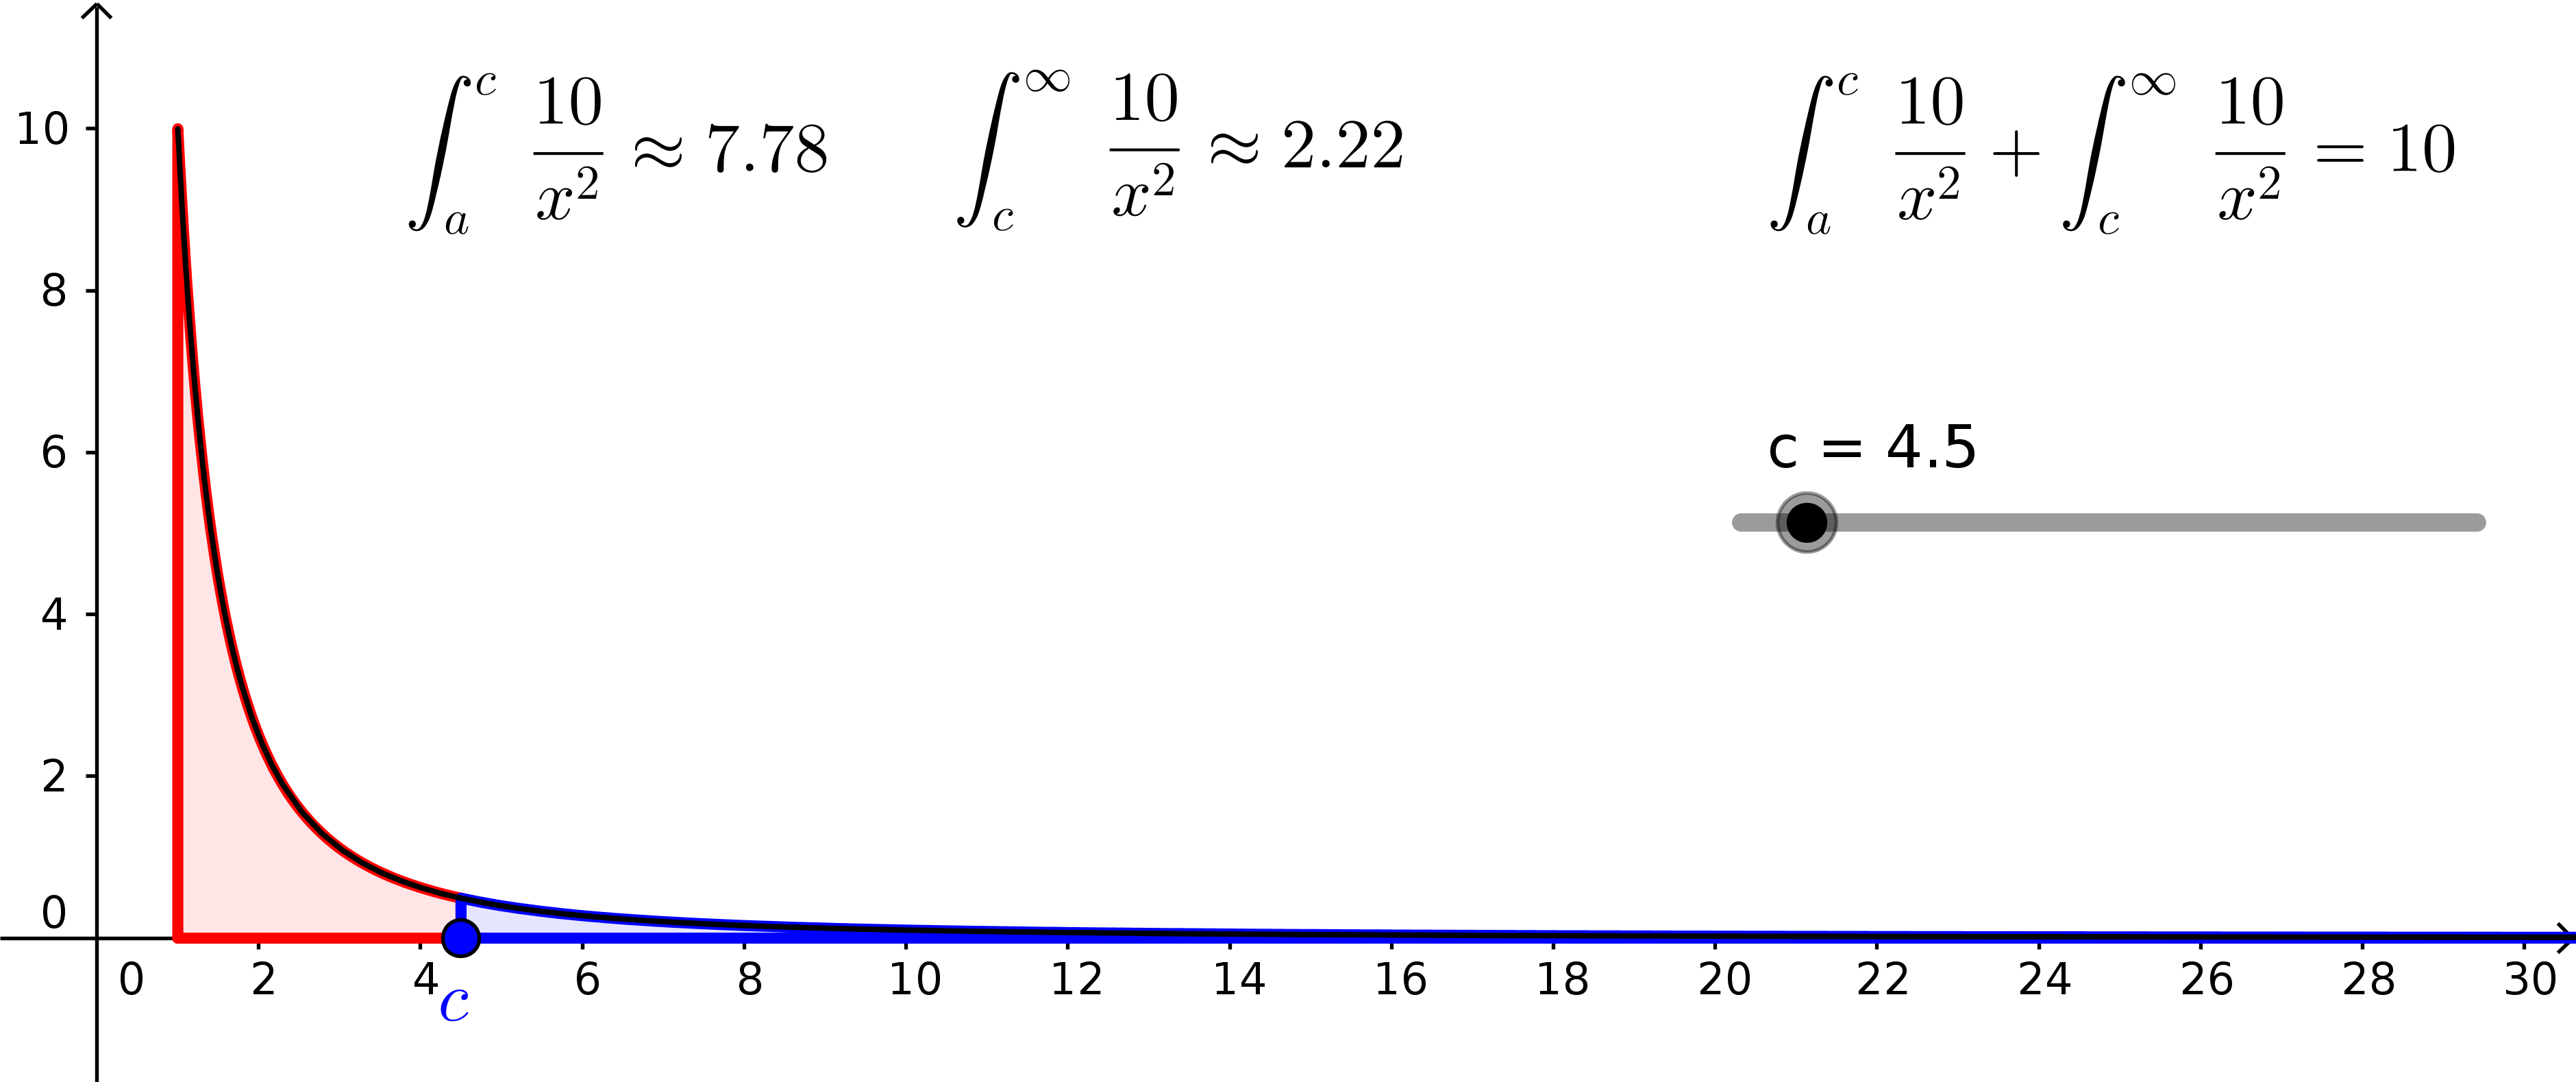
\includegraphics[width=12cm,keepaspectratio=true]{07_samleitidheildi.png}
\end{center}



\subsection{Setning}
\label{kafli06:id11}
Látum \(-\infty\leq a<b\leq \infty\). Gerum ráð fyrir að föllin
\(f\) og \(g\) séu samfelld á \((a, b)\) og að um öll
\(x\in (a, b)\) gildi að \(0\leq f(x)\leq g(x)\).
\begin{enumerate}
\item {} 
Ef heildið \(\int_a^b g(x)\,dx\) er samleitið þá er heildið
\(\int_a^b f(x)\,dx\) líka samleitið og
\begin{equation*}
\begin{split}\int_a^b f(x)\,dx \leq \int_a^b g(x)\,dx.\end{split}
\end{equation*}
\item {} 
Ef heildið \(\int_a^b f(x)\,dx\) er ósamleitið þá er heildið
\(\int_a^b g(x)\,dx\) líka ósamleitið.

\end{enumerate}


\chapter{Rúmmál, massi og massamiðja}
\label{kafli07:rummal-massi-og-massamija}\label{kafli07::doc}
\emph{The fact that we live at the bottom of a deep gravity well, on the surface of a
gas covered planet going around a nuclear fireball 90 million miles away and think
this to be normal is obviously some indication of how skewed our perspective tends to be.}

- Douglas Adams, The Salmon of Doubt: Hitchhiking the Galaxy One Last Time

\index{rúmmál}

\section{Rúmmál, lengd og flatarmál}
\label{kafli07:rummal-lengd-og-flatarmal}\label{kafli07:index-1}

\subsection{Rúmmál rúmskika}
\label{kafli07:rummal-rumskika}
Rúmskiki \(D\) liggur á milli plananna \(x=a\) og \(x=b\).
Táknum með \(A(x)\) flatarmál þversniðs \(D\) við plan sem sker
\(x\)-ásinn í \(x\) og er hornrétt á \(x\)-ás. Ef fallið
\(A(x)\) er heildanlegt yfir bilið \([a, b]\) þá er rúmmál
\(D\) jafnt og
\begin{equation*}
\begin{split}V=\int_a^b A(x)\,dx.\end{split}
\end{equation*}
\index{rúmmál!keilu}

\subsection{Rúmmál keilu}
\label{kafli07:rummal-keilu}\label{kafli07:index-2}
Látum \(F\) vera takmarkaðan samanhangandi bút af plani og látum
\(T\) vera punkt sem liggur ekki í planinu. Látum \(A\) tákna
flatarmál \(F\) og \(h\) tákna fjarlægð topppunktsins frá
planinu sem grunnflöturinn liggur í. \textit{Keila} með grunnflöt \(F\) og
topppunkt \(T\) er rúmskiki sem afmarkast af grunnfletinum \(F\)
og öllum strikum sem liggja frá punktum á jaðri \(F\) til \(T\).
Rúmmál keilunnar er
\begin{equation*}
\begin{split}V=\frac{1}{3}hA=\frac{1}{3}(\mbox{hæð})(\mbox{flatarmál
grunnflatar}).\end{split}
\end{equation*}
Formúlan gildir óháð lögun grunnflatarins \(F\).

\index{rúmmál!snúðs}\index{snúið um x-ás}

\subsection{Rúmmál snúðs, snúið um \protect\(x\protect\)-ás}
\label{kafli07:rummal-snus-snui-um-as}\label{kafli07:index-3}
Látum \(f\) vera samfellt fall á bili \([a, b]\). Rúmskikinn sem
myndast þegar svæðinu sem afmarkast af \(x\)-ás, grafinu
\(y=f(x)\) og línunum \(x=a\) og \(x=b\) er snúið
\(360^\circ\) um \(x\)-ás hefur rúmmálið
\begin{equation*}
\begin{split}V=\pi\int_a^b f(x)^2\,dx.\end{split}
\end{equation*}
Sjá  \href{https://www.geogebra.org/m/40798}{3D volume by rotation of a function} (https://www.geogebra.org/m/40798)
eftir \href{https://www.geogebra.org/material/show/id/40798}{George Katehos} (https://www.geogebra.org/material/show/id/40798) (CC-BY-SA).

\index{rúmmál!snúðs með gati}

\subsection{Rúmmál snúðs með gati}
\label{kafli07:rummal-snus-me-gati}\label{kafli07:index-4}
Látum \(f\) og \(g\) vera tvö samfelld föll skilgreind á bilinu
\([a, b]\). Gerum ráð fyrir að um öll \(x\in [a, b]\) gildi að
\(0\leq f(x)\leq
g(x)\). Þegar svæðinu milli grafa \(f\) og \(g\) er snúið
\(360^\circ\) um \(x\)-ás fæst rúmskiki sem hefur rúmmálið
\begin{equation*}
\begin{split}V=\pi\int_a^b g(x)^2-f(x)^2\,dx.\end{split}
\end{equation*}
\index{rúmmál!snúðs}\index{snúið um y-ás}

\subsection{Rúmmál snúðs, snúið um \protect\(y\protect\)-ás}
\label{kafli07:index-5}\label{kafli07:id1}
Látum \(f\) vera samfellt fall skilgreint á bili \([a, b]\), með
\(a<b\). Gerum ráð fyrir að \(f(x)\geq 0\) fyrir öll
\(x\in [a, b]\). Rúmmál rúmskikans sem fæst með að snúa svæðinu sem
afmarkast af \(x\)-ás, grafinu \(y=f(x)\) og línunum \(x=a\)
og \(x=b\) um \(360^\circ\) um \(y\)-ás er
\begin{equation*}
\begin{split}V=2\pi\int_a^b xf(x)\,dx.\end{split}
\end{equation*}
\index{fall!lengd grafs}
Sjá \href{https://www.geogebra.org/b/75281\#material/18475}{Solids and volumes of revolution (rotation about y\_axis)} (https://www.geogebra.org/b/75281\#material/18475)
eftir \href{https://www.geogebra.org/b/75281\#material/18475}{George Katehos} (https://www.geogebra.org/b/75281\#material/18475) (CC-BY-SA).


\subsection{Lengd grafs}
\label{kafli07:lengd-grafs}
Látum \(f\) vera samfellt fall skilgreint á bili \([a, b]\).
Lengd grafsins \(y=f(x)\) milli \(x=a\) og \(x=b\) er
skilgreind sem
\begin{equation*}
\begin{split}s=\int_a^b\sqrt{1+(f'(x))^2}\,dx.\end{split}
\end{equation*}
\index{flatarmál!yfirborðsflatarmál snúðs}\index{snúið um x-ás}

\subsection{Yfirborðsflatarmál snúðs, snúið um \protect\(x\protect\)-ás}
\label{kafli07:yfirborsflatarmal-snus-snui-um-as}\label{kafli07:index-7}
Látum \(f\) vera samfellt fall skilgreint á bili \([a, b]\).
Grafinu \(y=f(x)\) er snúið \(360^\circ\) um \(x\)-ás og
myndast við það flötur. Flatarmál flatarins er gefið með formúlunni
\begin{equation*}
\begin{split}S=2\pi\int_a^b|f(x)|\sqrt{1+(f'(x))^2}\,dx.\end{split}
\end{equation*}
\index{flatarmál!yfirborðsflatarmál snúðs}\index{snúið um y-ás}

\subsection{Yfirborðsflatarmál snúðs, snúið um \protect\(y\protect\)-ás}
\label{kafli07:id3}\label{kafli07:index-8}
Látum \(f\) vera samfellt fall skilgreint á bili \([a, b]\).
Grafinu \(y=f(x)\) er snúið \(360^\circ\) um \(y\)-ás og
myndast við það flötur. Flatarmál flatarins er gefið með formúlunni
\begin{equation*}
\begin{split}S=2\pi\int_a^b|x|\sqrt{1+(f'(x))^2}\,dx.\end{split}
\end{equation*}
\index{massi}

\section{Massi}
\label{kafli07:index-9}\label{kafli07:massi}
\index{massi!vírs}\index{massi!massafrymi}

\subsection{Massi vírs}
\label{kafli07:massi-virs}\label{kafli07:index-10}
Vír liggur eftir ferli \(y=f(x)\) þar sem \(a\leq x\leq b\).
Efnisþéttleiki (eðlisþyngdin) í punkti \((x, f(x))\) er gefinn sem
\(\delta(x)\). \emph{Massafrymi} vírsins (massi örbúts af lengd
\(ds\)) er
\begin{equation*}
\begin{split}dm
= \delta(x)\, ds
=\delta(x)\sqrt{1+(f'(x))^2}\, dx,\end{split}
\end{equation*}
og massi alls vírsins er
\begin{equation*}
\begin{split}m=\int_a^b \delta(x)\,ds=\int_a^b \delta(x)\sqrt{1+(f'(x))^2}\, dx.\end{split}
\end{equation*}
\index{massi!plötu}

\subsection{Massi plötu}
\label{kafli07:index-11}\label{kafli07:massi-plotu}\label{kafli07:id4}
Plata afmarkast af \(x\)-ás, grafinu \(y=f(x)\) og línunum
\(x=a\) og \(x=b\). Á línu sem er hornrétt á \(x\)-ás og
sker \(x\)-ásinn í \(x\) er efnisþéttleikinn fastur og gefinn
með \(\delta(x)\).

Flatarmál örsneiðar milli lína hornréttra á \(x\)-ás sem skera ásinn
í \(x\) og \(x+dx\) er \(dA=f(x)\,dx\).

Massafrymi fyrir plötuna (massi örsneiðarinnar) er
\begin{equation*}
\begin{split}dm =\delta(x)dA = \delta(x) f(x)\,dx,\end{split}
\end{equation*}
og massi allrar plötunnar er
\begin{equation*}
\begin{split}m=\int_a^b \delta(x)f(x)\,dx.\end{split}
\end{equation*}
\index{massi!rúmskika}

\subsection{Massi rúmskika}
\label{kafli07:index-12}\label{kafli07:massi-rumskika}
Rúmskiki \(D\) liggur á milli plananna \(x=a\) og \(x=b\).
Táknum með \(A(x)\) flatarmál þversniðs \(D\) við plan sem sker
\(x\)-ásinn í \(x\) og er hornrétt á \(x\)-ás. Gerum ráð
fyrir að efnisþéttleikinn sé fastur á hverju þversniði, og að á
þversniði \(D\) við plan sem sker \(x\)-ásinn í \(x\) og er
hornrétt á \(x\)-ás sé efnisþéttleikinn gefinn með
\(\delta(x)\).

Rúmmálsfrymi (rúmmál örsneiðar úr \(D\) sem liggur á milli tveggja
plana sem eru hornrétt á \(x\)-ásinn og skera \(x\)-ásinn í
\(x\) og \(x+dx\)) er \(dV=A(x)\, dx\).

Massafrymi (massi örsneiðarinnar) er
\begin{equation*}
\begin{split}dm=\delta(x)\, dV = \delta(x) A(x)\, dx,\end{split}
\end{equation*}
og massi rúmskikans \(D\) er þá
\begin{equation*}
\begin{split}m=\int_a^b \delta(x)A(x)\, dx.\end{split}
\end{equation*}
\index{massi!massamiðja}\index{massi!vægi}

\section{Massamiðja}
\label{kafli07:index-13}\label{kafli07:massamija}

\subsection{Skilgreining: Massamiðja punktmassa}
\label{kafli07:skilgreining-massamija-punktmassa}
Punktmassar \(m_1, m_2, \ldots, m_n\) eru staðsettir í punktunum
\(x_1,
x_2, \ldots, x_n\) á \(x\)-ásnum.

\textit{Vægi} kerfisins um punktinn \(x=0\) er skilgreint sem
\begin{equation*}
\begin{split}M_{x=0}=\sum_{i=1}^n x_im_i,\end{split}
\end{equation*}
og \textit{massamiðja} kerfisins er
\begin{equation*}
\begin{split}\overline{x}=\frac{M_{x=0}}{m} = \frac{\sum_{i=1}^n x_im_i}{\sum_{i=1}^n m_i}.\end{split}
\end{equation*}

\subsection{Skilgreining: Massamiðja}
\label{kafli07:skilgreining-massamija}
Ef massi er dreifður samkvæmt þéttleika falli \(\delta(x)\) um bil
\([a, b]\) á \(x\)-ásnum þá er massi og vægi um punktinn
\(x=0\) gefið með formúlunum
\begin{equation*}
\begin{split}m=\int_a^b \delta(x)\,dx
\qquad\mbox{ og }\qquad
M_{x=0}= \int_a^b x\delta(x)\,dx.\end{split}
\end{equation*}
Massamiðjan er gefin með formúlunni
\begin{equation*}
\begin{split}\overline{x}=\frac{M_{x=0}}{m}   =
\frac{\int_a^b x\delta(x)\,dx}{\int_a^b \delta(x)\,dx}.\end{split}
\end{equation*}
\index{massi!massamiðja plötu}

\subsection{Skilgreining: Massamiðja plötu}
\label{kafli07:index-14}\label{kafli07:skilgreining-massamija-plotu}
Skoðum plötu af sömu gerð og í {\hyperref[kafli07:massi\string-plotu]{\sphinxcrossref{\DUrole{std,std-ref}{7.2.2}}}}.

Vægi plötunnar um \(y\)- og \(x\)-ása eru gefin með formúlunum
\begin{equation*}
\begin{split}M_{x=0}=\int_a^b x\delta(x)f(x)\,dx
\qquad\mbox{og}\qquad
M_{y=0}=\frac{1}{2}\int_a^b \delta(x)f(x)^2\,dx,\end{split}
\end{equation*}
og hnit massamiðju plötunnar, \((\overline{x}, \overline{y})\), eru
gefin með jöfnunum
\begin{equation*}
\begin{split}\overline{x}=\frac{M_{x=0}}{m}=
\frac{\int_a^b x\delta(x)f(x)\,dx}{\int_a^b \delta(x)f(x)\,dx}\end{split}
\end{equation*}
og
\begin{equation*}
\begin{split}\overline{y}=\frac{M_{y=0}}{m}=
\frac{\frac{1}{2}\int_a^b \delta(x)f(x)^2\,dx}{\int_a^b
\delta(x)f(x)\,dx}.\end{split}
\end{equation*}
\index{setning Pappusar}

\subsection{Setning Pappusar, I}
\label{kafli07:setning-pappusar-i}\label{kafli07:index-15}
Látum \(R\) vera svæði sem liggur í plani öðrum megin við línu
\(L\). Látum \(A\) tákna flatarmál \(R\) og
\(\overline{r}\) tákna fjarlægð massamiðju \(R\) frá \(L\).

Þegar svæðinu \(R\) er snúið \(360^\circ\) um \(L\) myndast
snúðskiki með rúmmál
\begin{equation*}
\begin{split}V=2\pi\overline{r}A.\end{split}
\end{equation*}

\subsection{Setning Pappusar, II}
\label{kafli07:setning-pappusar-ii}
Látum \(C\) vera lokaðan feril sem liggur í plani og er allur öðrum
megin við línu \(L\). Látum \(s\) tákna lengd \(C\) og
\(\overline{r}\) tákna fjarlægð massamiðju \(C\) frá \(L\).
Þegar ferlinum \(C\) er snúið \(360^\circ\) um \(L\) myndast
snúðflötur með flatarmál
\begin{equation*}
\begin{split}S=2\pi\overline{r}s.\end{split}
\end{equation*}

\chapter{Diffurjöfnur}
\label{kafli08:diffurjofnur}\label{kafli08::doc}
\emph{Now, the invention of the scientific method and science is, I'm sure
we'll all agree, the most powerful intellectual idea, the most powerful
framework for thinking and investigating and understanding and challenging
the world around us that there is, and that it rests on the premise that
any idea is there to be attacked and if it withstands the attack then it
lives to fight another day and if it doesn't withstand the attack then
down it goes.}

-- Douglas Adams

\index{diffurjafna}\index{afleiðujafna|see{diffurjafna}}\index{deildajafna|see{diffurjafna}}\index{diffurjafna!stig}

\section{Diffurjöfnur}
\label{kafli08:index-0}\label{kafli08:id1}

\subsection{Skilgreining: Diffurjafna}
\label{kafli08:skilgreining-diffurjafna}\label{kafli08:diffurjafna}
Ritum \(y=y(x)\) sem fall af \(x\).

\textit{Diffurjafna} er jafna á forminu
\begin{equation*}
\begin{split}F(x, y, y', y'', \ldots, y^{(n)})=0\end{split}
\end{equation*}
þar sem \(F\) er fall (formúla) í \(n+1\) breytistærð.

Jafnan er sögð vera af \(n\)-ta \emph{stigi} ef hæsta afleiða \(y\)
sem kemur fyrir í formúlu er \(n\).

Að leysa diffurjöfnu felur í sér að skrifa \(y\) sem fall
af \(x\), þ.e. finna formúlu fyrir \(y\).

\begin{notice}{note}{Athugasemd:}
Deildajafna, afleiðujafna og diffurjafna eru samheiti yfir
sama hlutinn.
\end{notice}


\subsection{Dæmi}
\label{kafli08:daemi}
Það að finna stofnfall fyrir gefið fall \(f\) er jafngilt því að leysa
fyrsta stigs diffurjöfnuna
\begin{equation*}
\begin{split}y'(x) = f(x),\end{split}
\end{equation*}
eða með framsetningunni úr {\hyperref[kafli08:diffurjafna]{\sphinxcrossref{\DUrole{std,std-ref}{skilgreiningunni}}}} hér
að ofan,
\begin{equation*}
\begin{split}F(x,y') = f(x) - y'(x) = 0.\end{split}
\end{equation*}
\index{diffurjafna!aðgreinanleg}

\subsection{Skilgreining: Aðgreinanleg diffurjafna}
\label{kafli08:skilgreining-agreinanleg-diffurjafna}\label{kafli08:index-1}
Fyrsta stigs diffurjafna sem má rita á forminu
\begin{equation*}
\begin{split}\frac{dy}{dx}=f(x)g(y)\end{split}
\end{equation*}
kallast \emph{aðgreinanleg}. Það er, þátta má hægri hliðina
þannig að annar þátturinn er bara fall af \(x\) og hinn þátturinn er
bara fall af \(y\).

Umritum jöfnuna yfir á formið
\begin{equation*}
\begin{split}\frac{dy}{g(y)}=f(x)\,dx.\end{split}
\end{equation*}
\begin{notice}{warning}{Aðvörun:}
Það má ekkert \(x\) koma fyrir í vinstri hliðinni og
ekkert \(y\) má koma fyrir í hægri hliðinni.
\end{notice}

Síðan heildum við báðar hliðar og reiknum stofnföllin hægra og vinstra
megin í jöfnunni
\begin{equation*}
\begin{split}\int\frac{dy}{g(y)}=\int f(x)\,dx.\end{split}
\end{equation*}
og munum eftir að setja inn heildunarfasta (einn er nóg). Þá höfum við
jöfnu sem lýsir sambandi \(x\) og \(y\), og inniheldur engar
afleiður af \(y\). Út frá þeirri jöfnu má fá upplýsingar um
eiginleika lausnarinnar \(y\). Stundum er hægt að einangra \(y\)
og fá þannig formúlu fyrir lausn diffurjöfnunar.


\subsection{Dæmi um aðgreinanlega diffurjöfnu}
\label{kafli08:daemi-um-agreinanlega-diffurjofnu}
Ef við skoðum diffurjöfnuna
\begin{equation*}
\begin{split}y' = x\exp(x-y)\end{split}
\end{equation*}
þá sjáum við að hún er aðgreinanleg því með því að skrifa \(\exp(x-y) = \exp (x) \exp(-y)\) og
margfalda í gegn með \(\exp (y)\) þá fæst
\begin{equation*}
\begin{split}\exp(y)\, y' = x\exp x.\end{split}
\end{equation*}
Hér eru öll \(y\) vinstra megin og öll \(x\) hægra megin.
Heildum nú beggja vegna og munum að það er nóg að setja einn heildunarfasta
\begin{equation*}
\begin{split}\exp{y} + C = \int \exp y \, dy = \int x\exp x\, dx = x\exp x - \exp x.\end{split}
\end{equation*}
Reynum nú að einangra \(y\) til þess að geta skrifað út formúlu fyrir lausninni.
Byrjum á að færa heildunarfastann yfir og tökum svo logrann af báðum hliðum
\begin{equation*}
\begin{split}y = \ln(x\exp x - \exp x - C).\end{split}
\end{equation*}
\index{diffurjafna!línuleg}

\section{Línulegar fyrsta stigs diffurjöfnur}
\label{kafli08:index-2}\label{kafli08:linulegar-fyrsta-stigs-diffurjofnur}
\index{diffurjafna!hliðruð}\index{diffurjafna!óhliðruð}

\subsection{Skilgreining: Línuleg diffurjafna}
\label{kafli08:skilgreining-linuleg-diffurjafna}\label{kafli08:index-3}
Diffurjafna á forminu
\begin{equation*}
\begin{split}a_n(x)y^{(n)}+a_{n-1}(x)y^{(n-1)}+\cdots+a_1(x)y'+a_0(x)y=f(x)\end{split}
\end{equation*}
kallast \textit{línuleg diffurjafna}. Hún er \(n\)-ta stigs ef
\(a_n(x)\) er ekki fastafallið \(0\).

Ef \(f\) er fastafallið \(0\) þá er jafnan sögð \textit{óhliðruð}
en ef \(f\) er ekki fastafallið \(0\) þá er hún
sögð \textit{hliðruð}.

\index{diffurjafna!fyrsta stigs}

\subsection{Línulegar fyrsta stigs diffurjöfnur}
\label{kafli08:id2}\label{kafli08:index-4}
Almenna línulega fyrsta stigs jöfnu má rita á forminu
\begin{equation*}
\begin{split}y'+p(x)y=q(x).\end{split}
\end{equation*}
Samsvarandi óhliðruð jafna er
\begin{equation*}
\begin{split}y'+p(x)y=0.\end{split}
\end{equation*}
Skilgreinum \(\mu(x)=\int p(x)\,dx\) (eitthvert stofnfall). Þá er
\begin{equation*}
\begin{split}y(x)=e^{-\mu(x)}\int e^{\mu(x)}q(x)\,dx\end{split}
\end{equation*}
lausn á diffurjöfnunni.

\begin{notice}{warning}{Aðvörun:}
Þegar þið reiknið \(\mu(x)=\int p(x)\,dx\) þá megið þið sleppa
heildunarfastanum, en \textbf{ekki} þegar þið reiknið heildið
\(\int e^{\mu(x)}q(x)\,dx\).
\end{notice}

\index{diffurjafna!annars stigs}
\textbf{Sönnun}

Setjum
\begin{equation*}
\begin{split}y(x)=e^{-\mu(x)}\int e^{\mu(x)}q(x)\,dx\end{split}
\end{equation*}
inn í vinstri hlið diffurjöfnunnar, ef út kemur hægri hliðin \(q(x)\) þá
höfum við sýnt að þetta er lausn.

Athugum fyrst að
\begin{equation*}
\begin{split}\begin{aligned}
y'(x) &=e^{-\mu(x)}(-\mu'(x)) \int e^{\mu(x)}q(x)\, dx + e^{-\mu(x)} \frac{d}{dx} \int e^{\mu(x)}q(x)\,dx \\
&= -e^{-\mu(x)}p(x)\int e^{\mu(x)}q(x)\, dx +  e^{-\mu(x)} e^{\mu(x)}q(x) = -p(x)y(x) + q(x).
\end{aligned}\end{split}
\end{equation*}
Ef við setjum þetta inn í diffurjöfnuna fæst
\begin{equation*}
\begin{split}y'(x) + p(x)y(x) = -p(x)y(x) + q(x) + p(x)y(x) = q(x),\end{split}
\end{equation*}
þannig að \(y\) skilgreint eins og hér að ofan er greinilega lausn á diffurjöfnunni.


\section{Línulegar annars stigs diffurjöfnur með fastastuðla}
\label{kafli08:linulegar-annars-stigs-diffurjofnur-me-fastastula}

\subsection{Skilgreining}
\label{kafli08:skilgreining}
\emph{Línuleg annars stigs diffurjafna með fastastuðla} er diffurjafna á
forminu
\begin{equation*}
\begin{split}ay''+by'+cy=f(x)\end{split}
\end{equation*}
þar sem \(a, b\) og \(c\) eru fastar.

Jafnan er sögð \emph{óhliðruð} ef fallið \(f(x)\) er
fastafallið 0.

\index{diffurjafna!kennijafna}

\subsection{Skilgreining: Kennijafna}
\label{kafli08:skilgreining-kennijafna}\label{kafli08:index-6}
Jafnan \(ar^2+br+c=0\) kallast \textit{kennijafna}
diffurjöfnunnar \(ay''+by'+cy=0\).


\subsection{Setning}
\label{kafli08:setning}
Ef föllin \(y_1(x)\) og \(y_2(x)\) eru lausnir á diffurjöfnunni
\(ay''+by'+cy=0\) þá er fallið
\begin{equation*}
\begin{split}y(x)=Ay_1(x)+By_2(x),\end{split}
\end{equation*}
þar sem \(A\) og \(B\) eru fastar, líka lausn.

Ef \(y_2(x)\) er ekki fastamargfeldi af \(y_1(x)\) þá má skrifa
\textbf{sérhverja} lausn \(y(x)\) á diffurjöfnunni \(ay''+by'+cy=0\)
á forminu
\begin{equation*}
\begin{split}y(x)=Ay_1(x)+By_2(x),\end{split}
\end{equation*}
þar sem \(A\) og \(B\) eru fastar.


\subsection{Setning}
\label{kafli08:id3}\label{kafli08:stigs-ohlidrud}
Ef leysa á annars stigs óhliðraða diffurjöfnu með fastastuðla
\begin{equation*}
\begin{split}ay''+by'+cy=0\end{split}
\end{equation*}
þá geta komið upp þrjú tilvik.
\begin{description}
\item[{Tilvik I}] \leavevmode
\emph{Kennijafnan} \(ar^2+br+c=0\) \emph{hefur tvær ólíkar rauntölulausnir}
\(r_1\) og \(r_2\).

Þá er fallið
\begin{equation*}
\begin{split}y(x)=Ae^{r_1x}+Be^{r_2x}\end{split}
\end{equation*}
alltaf lausn sama hvernig fastarnir \(A\) og \(B\) eru
valdir og sérhverja lausn má rita á þessu formi.

\item[{Tilvik II}] \leavevmode
\emph{Kennijafnan} \(ar^2+br+c=0\) \emph{hefur bara eina rauntölulausn}
\(k=-\frac{b}{2a}\).

Þá er fallið
\begin{equation*}
\begin{split}y(x)=Ae^{kx}+Bxe^{kx}\end{split}
\end{equation*}
alltaf lausn sama hvernig fastarnir \(A\) og \(B\) eru
valdir og sérhverja lausn má rita á þessu formi.

\item[{Tilvik III}] \leavevmode
\emph{Kennijafnan} \(ar^2+br+c=0\) \emph{hefur engar rauntölulausnir.}

Setjum \(k=-\frac{b}{2a}\) og
\(\omega=\frac{\sqrt{4ac-b^2}}{2a}\).

Rætur kennijöfnunnar eru \(r_1=k+i\omega\) og
\(r_2=k-i\omega\).

Þá er fallið
\begin{equation*}
\begin{split}y(x)=Ae^{kx}\cos(\omega x)+Be^{kx}\sin(\omega x)\end{split}
\end{equation*}
alltaf lausn sama hvernig fastarnir \(A\) og \(B\) eru
valdir og sérhverja lausn má rita á þessu formi.

\end{description}


\subsection{Setning}
\label{kafli08:id4}
Látum \(y_{\rm p}(x)\) vera einhverja lausn á hliðruðu jöfnunni
\begin{equation*}
\begin{split}ay''+by'+cy=f(x).\end{split}
\end{equation*}
Látum \(y_1(x)\) og \(y_2(x)\) vera lausnir sem fást úr {\hyperref[kafli08:stigs\string-ohlidrud]{\sphinxcrossref{\DUrole{std,std-ref}{8.3.4}}}} á
óhliðruðu jöfnunni
\begin{equation*}
\begin{split}ay''+by'+cy=0.\end{split}
\end{equation*}
Sama hvernig fastarnir \(A\) og \(B\) eru valdir þá er fallið
\begin{equation*}
\begin{split}y(x)=Ay_1(x)+By_2(x)+y_{\rm p}(x)\end{split}
\end{equation*}
alltaf lausn á diffurjöfnunni \(ay''+by'+cy=f(x)\) og sérhverja
lausn má skrifa á þessu formi.


\section{Ágiskanir}
\label{kafli08:agiskanir}
Við höfum skoðað aðferðir til að leysa aðgreinanlegar diffurjöfnur,
línulegar fyrsta stigs diffurjöfnur og óhliðraðar línulegar
annars stigs diffurjöfnur með fastastuðla. Þessar jöfnur eru
samt bara pínulítið brot af öllum mögulegum diffurjöfnum og ef við
veljum diffurjöfnu af ``handahófi'' þá getum við yfirleitt ekki
leyst hana auðveldlega.

Þrátt fyrir þetta er ástæðulaust að gefast upp og fyrir ákveðinn flokk
af diffurjöfnum þá getum við stundum giskað á lausn, en þetta eru
\textbf{hliðraðar} línulegar annars stigs diffurjöfnur með fastastuðla.

\index{diffurjafna!ágiskun}\index{diffurjafna!sérlausn}

\subsection{Ágiskun}
\label{kafli08:agiskun}\label{kafli08:id5}\label{kafli08:index-7}
Lausn á hliðruðu jöfnu \(ay''+by'+cy=f(x)\) kallast \emph{sérlausn}.
Stundum, ef \(f\) er ekki of flókið, þá er mögulegt að giska á sérlausn.

Látum \(P_n(x)\) standa fyrir einhverja \(n\)-ta stigs margliðu
og látum \(A_n(x)\) og \(B_n(x)\) tákna \(n\)-ta stigs
margliður með óákveðnum stuðlum.
\begin{itemize}
\item {} 
Ef \(f(x)=P_n(x)\) þá er giskað á \(y_{\rm p}(x)=x^mA_n(x)\).

\item {} 
Ef \(f(x)=P_n(x)e^{rx}\) þá er giskað á
\(y_{\rm p}(x)=x^mA_n(x)e^{rx}\).

\item {} 
Ef \(f(x)=P_n(x)e^{rx}\sin(kx)\) þá er giskað á
\(y_{\rm p}(x)=x^me^{rx}[A_n(x)\cos(kx)+B_n(x)\sin(kx)]\).

\item {} 
Ef \(f(x)=P_n(x)e^{rx}\cos(kx)\) þá er giskað á
\(y_{\rm p}(x)=x^me^{rx}[A_n(x)\cos(kx)+B_n(x)\sin(kx)]\).

\end{itemize}

Hér táknar \(m\) minnstu töluna af tölunum 0, 1, 2 sem tryggir að
enginn liður í ágiskuninni sé lausn á óhliðruðu jöfnunni
\(ay''+by'+cy=0\).

Ef við erum búin að finna sérlausn \(y_p\) og almenna lausn
\(y\) á óhliðruðu jöfnunni \(ay''+by'+cy=0\), þá er
\(y+y_p\) áfram lausn á hliðruðu jöfnunni. Reyndar er \textbf{sérhver}
lausn á óhliðruðu jöfnunni á forminu \(y+y_p\), bara
með mismundandi \(A\) og \(B\) í \(y\).


\section{Samantekt}
\label{kafli08:index-8}\label{kafli08:samantekt}

\subsection{Aðskiljanlegar jöfnur}
\label{kafli08:askiljanlegar-jofnur}
Jöfnur sem hægt er að rita á forminu
\begin{equation*}
\begin{split}\frac{dy}{dx} = f(x)g(y),\end{split}
\end{equation*}
má leysa með því að heilda og einangra \(y\) út úr
\begin{equation*}
\begin{split}\int \frac 1{g(y)}\, dy = \int f(x)\, dx.\end{split}
\end{equation*}

\subsection{Línulegar fyrsta stigs jöfnur}
\label{kafli08:linulegar-fyrsta-stigs-jofnur}
Lausn við jöfnu á forminu
\begin{equation*}
\begin{split}y'(x) + p(x)y = q(x)\end{split}
\end{equation*}
er gefin með
\begin{equation*}
\begin{split}y(x) = e^{-\mu(x)} \int e^{\mu(x)} q(x)\, dx,\end{split}
\end{equation*}
þar sem \(\mu(x) = \int p(x)\, dx\).


\subsection{Línulegar annars stigs jöfnur með fastastuðla}
\label{kafli08:linulegar-annars-stigs-jofnur-me-fastastula}
Lausn á \(ay''+by'+cy=0\) er gefin með
\begin{description}
\item[{Tilvik I}] \leavevmode
\(y(x)=Ae^{r_1x}+Be^{r_2x}\)
ef kennijafnan hefur tvær ólíkar rauntölulausnir \(r_1\) og
\(r_2\).

\item[{Tilvik II}] \leavevmode
\(y(x)=Ae^{kx}+Bxe^{kx}\)
ef kennijafnan \(ar^2+br+c=0\) hefur bara eina tvöfalda rauntölulausn
\(k=-\frac{b}{2a}\).

\item[{Tilvik III}] \leavevmode
\(y(x)=Ae^{kx}\cos(\omega x)+Be^{kx}\sin(\omega x)\)
ef kennijafnan \(ar^2+br+c=0\) hefur engar rauntölulausnir,
bara tvinntölulausnir \(r_1=k+i\omega\) og
\(r_2=k-i\omega\), þar sem
\(k=-\frac{b}{2a}\) og \(\omega=\frac{\sqrt{4ac-b^2}}{2a}\).

\end{description}

Lausn á liðruðu jöfnunni  á \(ay''+by'+cy=f(x)\) er mögulega hægt að finna
með {\hyperref[kafli08:agiskun]{\sphinxcrossref{\DUrole{std,std-ref}{ásgiskun}}}}. Sérhver lausn á óhliðruðu jöfnunni \(ay''+by'+cy=f(x)\)
er svo á forminu \(y+y_p\) þar sem \(y\) er
lausn á óhliðruðu jöfnunni.


\chapter{Runur og raðir}
\label{kafli09:runur-og-rair}\label{kafli09::doc}
\emph{Would it save you a lot of time if I just gave up and went mad now?}

- Douglas Adams, The Hitchhiker's Guide to the Galaxy

\index{runa}

\section{Runur}
\label{kafli09:index-0}\label{kafli09:runur}

\subsection{Skilgreining: Runa}
\label{kafli09:skilgreining-runa}
\emph{Runa} er raðaður listi af tölum.

Runa hefur fyrsta stak en ekkert síðasta stak. Stökin í runu eru oft
númeruð með náttúrlegu tölunum \(1, 2, 3, \ldots\). Stökin eru þá
\begin{equation*}
\begin{split}a_1, a_2, a_3, a_4, a_5, \ldots\end{split}
\end{equation*}
Runur eru táknaðar með \(\{a_n\}_{n\in {{{\mathbb  N}}}}\),
\(\{a_n\}_{n=1}^\infty\) eða bara \(\{a_n\}\).

Oft er runa gefin með formúlu, \(a_n = f(n)\). Til dæmis
\(a_n = 3n + n^2\).

\index{runa!takmörkuð}

\subsection{Skilgreining}
\label{kafli09:skilgreining}\label{kafli09:index-1}
Runa \(\{a_n\}\) er sögð \emph{takmörkuð að neðan} ef til er tala
\(m\) þannig að
\begin{equation*}
\begin{split}m\leq a_n\end{split}
\end{equation*}
fyrir allar náttúrlegar tölur \(n\).

Runan er sögð \emph{takmörkuð að ofan} ef til er tala \(M\) þannig að
\begin{equation*}
\begin{split}a_n\leq M\end{split}
\end{equation*}
fyrir allar náttúrlegar tölur \(n\).

Runa sem er bæði takmörkuð að ofan og neðan er sögð \emph{takmörkuð}.

\index{runa!vaxandi/minnkandi}\index{runa!einhalla}

\subsection{Skilgreining}
\label{kafli09:index-2}\label{kafli09:id1}
Runa \(\{a_n\}\) er sögð
\begin{enumerate}
\item {} 
\emph{vaxandi} ef \(a_n\leq a_{n+1}\) fyrir öll \(n\),

\item {} 
\emph{stranglega vaxandi} ef \(a_n< a_{n+1}\) fyrir öll \(n\),

\item {} 
\emph{minnkandi} ef \(a_n\geq a_{n+1}\) fyrir öll \(n\),

\item {} 
\emph{stranglega minnkandi} ef \(a_n> a_{n+1}\) fyrir öll
\(n\).

\end{enumerate}

Runa kallast \emph{einhalla} ef hún er annaðhvort vaxandi eða minnkandi.

\index{runa!víxlmerkjaruna}

\subsection{Skilgreining: Víxlmerkjaruna}
\label{kafli09:skilgreining-vixlmerkjaruna}\label{kafli09:index-3}
\emph{Víxlmerkjaruna} er runa þannig að formerki skiptast á, annaðhvort
\(+, -, +, -, \ldots\) eða \(-, +, -, +, \ldots\).

Einnig má lýsa þessu þannig að runa \(\{a_n\}\) sé víxlmerkjaruna ef
\(a_na_{n+1}<0\) fyrir öll \(n\).

\index{runa!samleitin}

\subsection{Skilgreining}
\label{kafli09:id2}\label{kafli09:index-4}
Segjum að \(\{a_n\}\) sé \emph{samleitin} að tölu \(L\) (eða \emph{stefni
á} \(L\)) ef fyrir sérhverja tölu \(\epsilon>0\) má finna
náttúrlega tölu \(N\) þannig að ef \(n\geq N\) þá er
\begin{equation*}
\begin{split}|a_n-L|<\epsilon.\end{split}
\end{equation*}
Ritað \(\lim_{n\rightarrow \infty}a_n=L\) og talan \(L\) kallast
\emph{markgildi rununnar}.

Sagt er að runa sé \emph{samleitin} ef \(\lim_{n\rightarrow \infty}a_n\)
er skilgreint, en annars er runan sögð \emph{ósamleitin}.


\subsection{Setning}
\label{kafli09:setning}
Látum \(f\) vera fall skilgreint á \({{\mathbb  R}}\) og látum
\(\{a_n\}\) vera runu þannig að \(a_n=f(n)\) fyrir öll
\(n\). Ef \(\lim_{x\rightarrow
\infty}f(x)=L\) þá er \(\lim_{n\rightarrow\infty}a_n=L\).

\begin{notice}{warning}{Aðvörun:}
Þetta gildir ekki í hina áttina, runan getur verið
samleitin án þess að fallið sé það.
\end{notice}


\subsection{Setning}
\label{kafli09:id3}
Látum \(\{a_n\}\) vera runu. Eftirfarandi tvö skilyrði eru jafngild:
\begin{enumerate}
\item {} 
\(\lim_{n\rightarrow\infty}a_n=L\),

\item {} 
fyrir sérhvert \(\epsilon>0\) eru aðeins endanlega margir liðir
rununnar \(\{a_n\}\) utan við bilið
\((L-\epsilon, L+\epsilon)\).

\end{enumerate}


\subsection{Fylgisetning}
\label{kafli09:fylgisetning}
Samleitin runa er takmörkuð.


\subsection{Setning}
\label{kafli09:id4}
Gerum ráð fyrir að runurnar \(\{a_n\}\) og \(\{b_n\}\) séu
samleitnar. Þá gildir:
\begin{enumerate}
\item {} 
\(\lim_{n\rightarrow\infty}(a_n\pm b_n)=
\lim_{n\rightarrow\infty}a_n\pm\lim_{n\rightarrow\infty}b_n\),

\item {} 
\(\lim_{n\rightarrow\infty}ca_n=
c\lim_{n\rightarrow\infty}a_n\), þar sem \(c\) er fasti,

\item {} 
\(\lim_{n\rightarrow\infty}(a_n b_n)=
(\lim_{n\rightarrow\infty}a_n)(\lim_{n\rightarrow\infty}b_n)\),

\item {} 
ef \(\lim_{n\rightarrow\infty}b_n\neq 0\) þá er
\(\lim_{n\rightarrow\infty}\frac{a_n}{b_n}=
\frac{\lim_{n\rightarrow\infty}a_n}{\lim_{n\rightarrow\infty}b_n}\),

\item {} 
ef \(a_n\leq b_n\) fyrir öll \(n\) sem eru nógu stór, þá
er
\begin{equation*}
\begin{split}\lim_{n\rightarrow\infty}a_n\leq\lim_{n\rightarrow\infty}b_n,\end{split}
\end{equation*}
(frasinn \emph{fyrir öll} \(n\) \emph{sem eru nógu stór} þýðir að til er
einhver tala \(N\) þannig að skilyrðið gildir fyrir öll
\(n\geq N\)),

\item {} 
(Klemmuregla) ef \(a_n\leq c_n\leq b_n\) fyrir öll \(n\)
sem eru nógu stór og
\(\lim_{n\rightarrow\infty}a_n=L=\lim_{n\rightarrow\infty}b_n\)
þá er runan \(\{c_n\}\) samleitin og
\begin{equation*}
\begin{split}\lim_{n\rightarrow\infty}c_n=L.\end{split}
\end{equation*}
\end{enumerate}


\subsection{Setning}
\label{kafli09:id5}
Takmörkuð einhalla (vaxandi eða minnkandi) runa er samleitin.

\index{röð}

\section{Raðir}
\label{kafli09:index-5}\label{kafli09:rair}

\subsection{Skilgreining: Röð}
\label{kafli09:skilgreining-ro}
Látum \(a_1, a_2, \ldots\) vera gefna runu. \textit{Röðin}
\begin{equation*}
\begin{split}\sum_{n=1}^\infty a_n  = a_1+a_2+a_3+\cdots\end{split}
\end{equation*}
er skilgreind sem formleg summa liðanna \(a_1, a_2, a_3, \ldots\).

\index{röð!samleitin}

\subsection{Skilgreining}
\label{kafli09:id6}\label{kafli09:index-6}
Fáum í hendurnar röð \(\sum_{n=1}^\infty a_n\) þar sem
\(a_1, a_2, \ldots\) eru tölur. Skilgreinum
\begin{equation*}
\begin{split}s_n=a_1+a_2+\cdots+a_n\end{split}
\end{equation*}
sem summa fyrstu \(n\) liða raðarinnar. Segjum að röðin
\(\sum_{n=1}^\infty a_n\) sé \textit{samleitin með summu} \(s\) ef
\begin{equation*}
\begin{split}\lim_{n\rightarrow\infty}s_n=s.\end{split}
\end{equation*}
Það er að segja, röðin er samleitin með summu \(s\) ef
\begin{equation*}
\begin{split}\lim_{n\rightarrow \infty}(a_1+a_2+\cdots+a_n)=s.\end{split}
\end{equation*}
Ritum þá
\begin{equation*}
\begin{split}\sum_{n=1}^\infty a_n=s.\end{split}
\end{equation*}

\subsection{Setning}
\label{kafli09:id7}
Ef \(A=\sum_{n=1}^\infty a_n\) og \(B=\sum_{n=1}^\infty b_n\),
þ.e. báðar raðirnar eru samleitnar, þá gildir að
\begin{enumerate}
\item {} 
ef \(c\) er fasti þá er \(\sum_{n=1}^\infty ca_n=cA\),

\item {} 
\(\sum_{n=1}^\infty (a_n\pm b_n)=A\pm B\),

\item {} 
ef \(a_n\leq b_n\) fyrir öll \(n\) þá er \(A\leq B\).

\end{enumerate}


\subsection{Setning}
\label{kafli09:id8}
Ef röð \(\sum_{n=1}^\infty a_n\) er samleitin þá er
\begin{equation*}
\begin{split}\lim_{n\rightarrow\infty}a_n=0.\end{split}
\end{equation*}

\subsection{Athugasemd}
\label{kafli09:athugasemd}
Ef \(\lim_{n \to \infty} a_n = 0\) þá ekki víst að röðin
\(\sum_{n=1}^\infty a_n\) sé samleitin.

\index{röð!kvótaröð}

\subsection{Dæmi: Kvótaröð}
\label{kafli09:daemi-kvotaro}\label{kafli09:index-7}
Röðin
\begin{equation*}
\begin{split}\sum_{n=0}^\infty a^n\end{split}
\end{equation*}
kallast \emph{kvótaröð}. Hún er samleitin ef \(-1<a<1\) og þá er
\begin{equation*}
\begin{split}\sum_{n=0}^\infty a^n = \frac{1}{1-a}.\end{split}
\end{equation*}
\index{röð!kíkisröð}

\subsection{Dæmi: Kíkisröð}
\label{kafli09:daemi-kikisro}\label{kafli09:index-8}
Röðin
\begin{equation*}
\begin{split}\sum_{n=1}^\infty \frac{1}{n(n-1)}\end{split}
\end{equation*}
kallast \emph{kíkisröð}. Hún er samleitin og
\begin{equation*}
\begin{split}\sum_{n=1}^\infty \frac{1}{n(n-1)} =1.\end{split}
\end{equation*}
\index{röð!samleitnipróf}

\section{Samleitnipróf fyrir raðir}
\label{kafli09:index-9}\label{kafli09:samleitniprof-fyrir-rair}

\subsection{Setning}
\label{kafli09:id9}
Ef \(\lim_{n\rightarrow\infty}a_n\) er ekki til eða
\(\lim_{n\rightarrow\infty}a_n\neq 0\) þá er röðin
\(\sum_{n=1}^\infty a_n\) ekki samleitin.


\subsection{Setning: Samleitnipróf I}
\label{kafli09:setning-samleitniprof-i}
Gerum ráð fyrir að \(a_n\geq 0\) fyrir allar náttúrlegar tölur
\(n\). Röðin \(\sum_{n=1}^\infty a_n\) er þá annaðhvort
samleitin eða ósamleitin að \(\infty\) (þ.e.a.s. hlutsummurnar
\(s_n=a_1+\cdots+a_n\) stefna á \(\infty\) þegar \(n\)
stefnir á \(\infty\).)


\subsection{Setning: Samleitnipróf II – Samanburðarpróf}
\label{kafli09:setning-samleitniprof-ii-samanburarprof}
Gerum ráð fyrir að \(0\leq a_n\leq b_n\) fyrir allar náttúrlegar
tölur \(n\).
\begin{enumerate}
\item {} 
Ef \(\sum_{n=1}^\infty b_n\) er samleitin þá er
\(\sum_{n=1}^\infty a_n\) líka samleitin.

\item {} 
Ef \(\sum_{n=1}^\infty a_n\) er ósamleitin þá er
\(\sum_{n=1}^\infty b_n\) líka ósamleitin.

\end{enumerate}


\subsection{Setning: Samleitnipróf III – Heildispróf}
\label{kafli09:setning-samleitniprof-iii-heildisprof}
Látum \(f\) vera \textbf{jákvætt, samfellt} og \textbf{minnkandi} fall sem er
skilgreint á bilinu \([1, \infty)\). Fyrir sérhverja náttúrlega tölu
\(n\) setjum við \(a_n=f(n)\). Þá eru röðin
\(\sum_{n=1}^\infty a_n\) og óeiginlega heildið
\(\int_1^\infty f(x)\,dx\) annaðhvort bæði samleitin eða bæði
ósamleitin.


\subsection{Fylgisetning}
\label{kafli09:id10}
Röðin \(\sum_{n=1}^\infty\frac{1}{n^{p}}\) er samleitin ef
\(p>1\) en ósamleitin ef \(p\leq 1\).


\subsection{Setning: Samleitnipróf IV – Markgildissamanburðarpróf}
\label{kafli09:setning-samleitniprof-iv-markgildissamanburarprof}
Gerum ráð fyrir að \(a_n\geq 0\) og \(b_n\geq 0\) fyrir allar
náttúrlegar tölur \(n\) og
\(\lim_{n\rightarrow\infty}\frac{a_n}{b_n}=L\), þar sem \(L\) er
tala eða \(\infty\).
\begin{enumerate}
\item {} 
Ef \(L<\infty\) og röðin \(\sum_{n=1}^\infty b_n\) er
samleitin þá er röðin \(\sum_{n=1}^\infty a_n\) líka samleitin.

\item {} 
Ef \(L>0\) og röðin \(\sum_{n=1}^\infty b_n\) er ósamleitin
þá er röðin \(\sum_{n=1}^\infty a_n\) líka ósamleitin.

\end{enumerate}


\subsection{Setning: Samleitnipróf V – Kvótapróf}
\label{kafli09:setning-samleitniprof-v-kvotaprof}
Gerum ráð fyrir að \(a_n>0\) fyrir öll \(n\) og að markgildið
\(\rho=\lim_{n\rightarrow\infty}\frac{a_{n+1}}{a_n}\) sé skilgreint
eða að það sé \(\infty\).
\begin{enumerate}
\item {} 
Ef \(0\leq\rho<1\) þá er röðin \(\sum_{n=1}^\infty a_n\)
samleitin.

\item {} 
Ef \(1<\rho\leq \infty\) þá er röðin
\(\sum_{n=1}^\infty a_n\) ósamleitin.

\item {} 
Ef \(\rho=1\) þá er ekkert hægt að fullyrða um hvort röðin
\(\sum_{n=1}^\infty a_n\) er samleitin eða ósamleitin, hvor
tveggja kemur til greina og nota þarf aðrar aðferðir til að skera
úr um það.

\end{enumerate}


\subsection{Setning: Samleitnipróf VI – Rótarpróf}
\label{kafli09:setning-samleitniprof-vi-rotarprof}
Gerum ráð fyrir að \(a_n>0\) fyrir öll \(n\) og að markgildið
\(\sigma=\lim_{n\rightarrow\infty}\sqrt[n]{a_n}\) sé skilgreint eða
að það sé \(\infty\).
\begin{enumerate}
\item {} 
Ef \(0\leq\sigma<1\) þá er röðin \(\sum_{n=1}^\infty a_n\)
samleitin.

\item {} 
Ef \(1<\sigma\leq \infty\) þá er röðin
\(\sum_{n=1}^\infty a_n\) ósamleitin.

\item {} 
Ef \(\sigma=1\) þá er ekkert hægt að fullyrða um hvort röðin
\(\sum_{n=1}^\infty a_n\) er samleitin eða ósamleitin, hvor
tveggja kemur til greina og nota þarf aðrar aðferðir til að skera
úr um það.

\end{enumerate}


\subsection{Setning: Samleitnipróf VII – Víxlmerkjaraðapróf}
\label{kafli09:setning-samleitniprof-vii-vixlmerkjaraaprof}\label{kafli09:vixlmerkjaprof}
Gerum ráð fyrir að
\begin{enumerate}
\item {} 
\(a_n\geq 0\) fyrir öll \(n\) (frekar jákvæðir liðir),

\item {} 
\(a_{n+1}\leq a_n\) fyrir öll \(n\) (frekar minnkandi),

\item {} 
\(\lim_{n\rightarrow\infty} a_n=0\) (stefnir á 0).

\end{enumerate}

Þá er víxlmerkjaröðin
\begin{equation*}
\begin{split}\sum_{n=1}^\infty (-1)^{n-1}a_n=a_1-a_2+a_3-a_4+\cdots\end{split}
\end{equation*}
samleitin.


\subsection{Fylgisetning}
\label{kafli09:id11}
Gerum ráð fyrir að runa \(\{a_n\}\) uppfylli skilyrðin sem gefin eru
í setningunni á undan {\hyperref[kafli09:vixlmerkjaprof]{\sphinxcrossref{\DUrole{std,std-ref}{(9.3.9)}}}}.

Látum \(s_n\) tákna summu \(n\) fyrstu liða raðarinnar
\(\sum_{n=1}^\infty (-1)^{n-1}a_n\) og táknum summu raðarinnar með
\(s\). Þá gildir að \(|s-s_n|\leq |a_{n+1}|\).

\index{röð!alsamleitni}

\section{Alsamleitni}
\label{kafli09:alsamleitni}\label{kafli09:index-10}

\subsection{Skilgreining}
\label{kafli09:id12}
Röð \(\sum_{n=1}^\infty a_n\) er sögð vera \emph{alsamleitin} ef röðin
\(\sum_{n=1}^\infty |a_n|\) er samleitin.


\subsection{Setning}
\label{kafli09:id13}
Röð sem er alsamleitin er samleitin.


\subsection{Athugasemd}
\label{kafli09:id14}
Til eru samleitnar raðir, t.d. röðin
\(\sum_{n=1}^\infty \frac{(-1)^{n-1}}{n}\), sem eru ekki
alsamleitnar.

\index{röð!skilyrt samleitni}

\subsection{Skilgreining}
\label{kafli09:index-11}\label{kafli09:id15}
Samleitin röð sem er ekki alsamleitin er sögð vera
\emph{skilyrt samleitin}, það er \(\sum_{n=1}^\infty a_n\) er samleitin
en röðin \(\sum_{n=1}^\infty |a_n|\) er ósamleitin.


\subsection{Setning: Umröðun}
\label{kafli09:setning-umroun}
Dæmi um umröðun á liðum raðar \(\sum_{n=1}^\infty a_n\) er
\begin{equation*}
\begin{split}a_{10}+a_9+\cdots+a_1+a_{100}+a_{99}+\cdots+a_{11}+
a_{1000}+a_{999}+\cdots.\end{split}
\end{equation*}\begin{enumerate}
\item {} 
Ef röðin \(\sum_{n=1}^\infty a_n\) er alsamleitin þá skiptir
engu máli hvernig liðum raðarinnar er umraðað, summan verður alltaf
sú sama.

\item {} 
Ef röðin \(\sum_{n=1}^\infty a_n\) er skilyrt samleitin og
\(L\) einhver rauntala, eða \(\pm\infty\) þá er hægt að
umraða liðum raðarinnar þannig að summan eftir umröðun verði
\(L\).

\end{enumerate}

\begin{notice}{note}{Athugasemd:}
Með öðrum orðum:
Liðum skilyrt samleitinnar raðar má umraða þannig að summan getur orðið
hvað sem er, það jskiptir því máli í hvaða röð við leggjum saman.
\end{notice}


\chapter{Veldaraðir}
\label{kafli10:veldarair}\label{kafli10::doc}
\emph{What to do if you find yourself stuck in a crack in the ground underneath
a giant boulder you can't move, with no hope of rescue. Consider how lucky
you are that life has been good to you so far. Alternatively, if life hasn't
been good to you so far, which given your current circumstances seems more
likely, consider how lucky you are that it won't be troubling you much longer.}

-- Douglas Adams, The Original Hitchhiker Radio Scripts

\index{veldaröð}\index{röð!veldaröð}

\section{Veldaraðir}
\label{kafli10:id1}\label{kafli10:index-1}

\subsection{Skilgreining}
\label{kafli10:skilgreining}
Röð á forminu
\begin{equation*}
\begin{split}\sum_{n=0}^\infty a_n(x-c)^n=a_0+a_1(x-c)+a_2(x-c)^2+\cdots\end{split}
\end{equation*}
kallast \textit{veldaröð} með \textit{miðju} í punktinum \(c\).


\subsection{Setning}
\label{kafli10:setning-samleitnigeisli}\label{kafli10:setning}
Um sérhverja veldaröð \(\sum_{n=0}^\infty a_n(x-c)^n\) gildir eitt
af þrennu:
\begin{enumerate}
\item {} 
Röðin er aðeins samleitin fyrir \(x=c\).

\item {} 
Til er jákvæð tala \(R\) þannig að veldaröðin er alsamleitin
fyrir öll \(x\) þannig að \(|x-c|<R\) og ósamleitin fyrir
öll \(x\) þannig að \(|x-c|>R\).

\item {} 
Röðin er samleitin fyrir allar rauntölur \(x\).

\end{enumerate}

\index{veldaröð!samleitnigeisli}\index{veldaröð!miðja}\index{veldaröð!samleitnibil}

\subsection{Skilgreining: Miðja og samleitnigeisli}
\label{kafli10:skilgreining-mija-og-samleitnigeisli}\label{kafli10:index-2}
Látum \(\sum_{n=0}^\infty a_n(x-c)^n\) vera veldaröð.
\begin{enumerate}
\item {} 
Talan \(c\) kallast \emph{miðja} eða \emph{samleitnimiðja}
veldaraðarinnar.

\item {} 
Í tilviki 2. í setningunni hér á undan er röðin alsamleitin á opna bilinu
\((c-R, c+R)\) og ósamleitin fyrir utan lokaða bilið
\([c-R, c+R]\).

Talan \(R\) er kölluð \textit{samleitnigeisli} raðarinnar.

Mögulegt er að röðin sé samleitin (alsamleitin eða skilyrt
samleitin) í öðrum eða báðum punktunum \(x=c-R\) og
\(x=c+R\) (þetta þarf að athuga sérstaklega).

Í tilfelli 1. í setningunni þegar röðin er bara samleitin fyrir \(x=c\)
setjum við \(R=0\) og í tilfelli 3. þegar röðin er
samleitin fyrir allar rauntölur \(x\) þá setjum við
\(R=\infty\).

\item {} 
\textit{Samleitnibil} veldaraðarinnar
\(\sum_{n=0}^\infty a_n(x-c)^n\) er mengi allra gilda
\(x\) þannig að röðin er samleitin. Setning hér á undan sýnir að
:þetta mengi er alltaf bil.
\begin{itemize}
\item {} 
Þegar samleitnigeilsinn er 0 er samleitnibilið \(\{c\}\).

\item {} 
Þegar samleitnigeislinn er \(R>0\) þá koma fjórir möguleikar
til greina eftir því hvort röðin er
samleitin í hvorugum, öðrum eða báðum punktunum \(x=c-R\) og
\(x=c+R\). Samleitnibilið getur verið
\((c-R, c+R)\), \([c-R, c+R)\), \((c-R, c+R]\) eða \([c-R, c+R]\).

\item {} 
Þegar samleitnigeislinn er \(\infty\) þá er samleitnibilið \((-\infty, \infty)\).

\end{itemize}

\end{enumerate}

\index{veldaröð!samleitnipróf}

\section{Samleitnipróf}
\label{kafli10:samleitniprof}\label{kafli10:index-3}

\subsection{Setning}
\label{kafli10:id2}
Látum \(\sum_{n=0}^\infty a_n(x-c)^n\) vera veldaröð.
\begin{enumerate}
\item {} 
\textit{Kvótapróf}: Gerum ráð fyrir að
\(L=\lim_{n\rightarrow\infty}\left|\frac{a_{n+1}}{a_n}\right|\)
sé til eða \(\infty\).

Þá hefur veldaröðin \(\sum_{n=0}^\infty a_n(x-c)^n\)
samleitnigeisla
\begin{equation*}
\begin{split}R= \left\{\begin{array}{ll}
\infty & \mbox{ef }L=0,\\
\frac{1}{L} & \mbox{ef }0<L<\infty,\\
0 & \mbox{ef }L=\infty.\\
\end{array} \right.\end{split}
\end{equation*}
\item {} 
\textit{Rótarpróf}: Gerum ráð fyrir að
\(L=\lim_{n\rightarrow\infty}\sqrt[n]{|a_n|}\) sé til eða
\(\infty\). Þá hefur veldaröðin
\(\sum_{n=0}^\infty a_n(x-c)^n\) samleitnigeisla
\begin{equation*}
\begin{split}R= \left\{\begin{array}{ll}
\infty & \mbox{ef }L=0,\\
\frac{1}{L} & \mbox{ef }0<L<\infty,\\
0 & \mbox{ef }L=\infty.\\
\end{array}
\right.\end{split}
\end{equation*}
\end{enumerate}

\index{setning Abels}

\subsection{Setning Abels}
\label{kafli10:setning-abels}\label{kafli10:index-4}
Fallið \(f\) skilgreint á samleitnibili með
\begin{equation*}
\begin{split}f(x)=\sum_{n=0}^\infty a_n(x-c)^n\end{split}
\end{equation*}
er samfellt á öllu samleitnibili veldaraðarinnar.

Ef samleitnigeislinn er \(0<R<\infty\) og röðin er samleitin í
punktinum \(x=c+R\) þá er
\begin{equation*}
\begin{split}\lim_{x\rightarrow (c+R)^-}f(x)=f(c+R)=\sum_{n=0}^\infty
a_n((c+R)-c)^n=\sum_{n=0}^\infty a_nR^n.\end{split}
\end{equation*}
Eins ef röðin er samleitin í punktinum \(x=c-R\) þá er
\begin{equation*}
\begin{split}\lim_{x\rightarrow (c-R)^+}f(x)=f(c-R)=\sum_{n=0}^\infty
a_n((c-R)-c)^n=\sum_{n=0}^\infty a_n(-R)^n.\end{split}
\end{equation*}

\subsection{Setning: Diffrað lið fyrir lið}
\label{kafli10:setning-diffra-li-fyrir-li}
Látum \(\sum_{n=0}^\infty a_n(x-c)^n=a_0+a_1(x-c)+a_2(x-c)^2+a_3(x-c)^3+\cdots\)
vera veldaröð með miðju í \(c\) og samleitnigeisla \(R\).

Fyrir \(x\in(c-R, c+R)\) skilgreinum við
\begin{equation*}
\begin{split}f(x)=\sum_{n=0}^\infty a_n(x-c)^n.\end{split}
\end{equation*}
Fallið \(f\) er diffranlegt og
\begin{equation*}
\begin{split}f'(x)=\sum_{n=1}^\infty na_n(x-c)^{n-1}=a_1+2a_2(x-c)+3a_3(x-c)^2+\cdots\end{split}
\end{equation*}
og röðin fyrir \(f'(x)\) er samleitin fyrir öll
\(x\in(c-R, c+R)\).

Þetta þýðir að við getum diffrað veldaraðir lið fyrir lið.

Þar sem diffranleg föll eru samfelld þá fæst eftirfarandi.


\subsection{Fylgisetning}
\label{kafli10:fylgisetning}
Fallið \(f\) er samfellt á \((c-R, c+R)\).


\subsection{Setning: Heildað lið fyrir lið}
\label{kafli10:setning-heilda-li-fyrir-li}
Látum
\(\sum_{n=0}^\infty a_n(x-c)^n=a_0+a_1(x-c)+a_2(x-c)^2+a_3(x-c)^3+\cdots\)
vera veldaröð með miðju í \(c\) og samleitnigeisla \(R\).

Fyrir \(x\in(c-R, c+R)\) skilgreinum við
\(f(x)=\sum_{n=0}^\infty a_n(x-c)^n\).

Fallið \(f\) hefur stofnfall
\begin{equation*}
\begin{split}\begin{gathered}
F(x)=\sum_{n=0}^\infty \frac{a_n}{n+1}(x-c)^{n+1} \\
=a_0(x-c)+\frac{a_1}{2}(x-c)^2+\frac{a_2}{3}(x-c)^3+
\frac{a_3}{4}(x-c)^4+\cdots\end{gathered}\end{split}
\end{equation*}
og röðin fyrir \(F(x)\) er samleitin fyrir öll
\(x\in(c-R, c+R)\).

Þetta þýðir að við getum heildað veldaraðir lið fyrir lið.


\subsection{Setning}
\label{kafli10:id3}
Látum \(\sum_{n=0}^\infty a_n(x-c)^n=a_0+a_1(x-c)+a_2(x-c)^2+a_3(x-c)^3+\cdots\)
vera veldaröð með miðju í \(c\) og samleitnigeisla \(R\).

Fyrir \(x\in(c-R, c+R)\) skilgreinum við
\begin{equation*}
\begin{split}f(x)=\sum_{n=0}^\infty a_n(x-c)^n.\end{split}
\end{equation*}
Fallið \(f\) er \(k\)-sinnum diffranlegt fyrir \(k=1, 2, 3, \ldots\) og
\begin{equation*}
\begin{split}a_k=\frac{f^{(k)}(c)}{k!}.\end{split}
\end{equation*}
\index{veldaröð!fágað fall}\index{fall!fágað}

\subsection{Skilgreining: Fágað fall}
\label{kafli10:skilgreining-faga-fall}\label{kafli10:index-5}
Fall \(f\) þannig að til er veldaröð
\(\sum_{n=0}^\infty a_n(x-c)^n\) með samleitnigeisla \(R>0\)
þannig að
\begin{equation*}
\begin{split}f(x)=\sum_{n=0}^\infty a_n(x-c)^n\end{split}
\end{equation*}
fyrir öll \(x\in(c-R, c+R)\) kallast \emph{fágað} (raunfágað) í punktinum
\(c\).


\subsection{Athugasemd}
\label{kafli10:athugasemd}
Dæmi um raunfáguð föll eru margliður, ræð föll, hornaföll, veldisföll og
lograr.

\index{Taylorröð}\index{veldaröð!Taylorröð}\index{Taylorröð!Maclaurinröð}

\section{Taylorraðir}
\label{kafli10:taylorrair}\label{kafli10:index-6}

\subsection{Skilgreining: Taylorröð}
\label{kafli10:skilgreining-taylorro}
Gerum ráð fyrir að fall \(f(x)\) sé óendanlega oft diffranlegt í
punktinum \(x=c\), (það er \(f^{(k)}(c)\) er til fyrir
\(k=0, 1, 2, \ldots\)).

Veldaröðin
\begin{equation*}
\begin{split}\begin{aligned}
\sum_{n=0}^\infty \frac{f^{(n)}(c)}{n!}(x-c)^n = & f(c)+f'(c)(x-c)+
\frac{f''(c)}{2}(x-c)^2 \\ & + \frac{f'''(c)}{3!}(x-c)^3
+ \frac{f^{(4)}(c)}{4!}(x-c)^4 + \cdots \end{aligned}\end{split}
\end{equation*}
kallast \emph{Taylorröð} með miðju í \(x=c\) fyrir \(f(x)\).

Ef svo vill til að \(c=0\) þá er oft talað um \emph{Maclaurinröð}.


\begin{center}
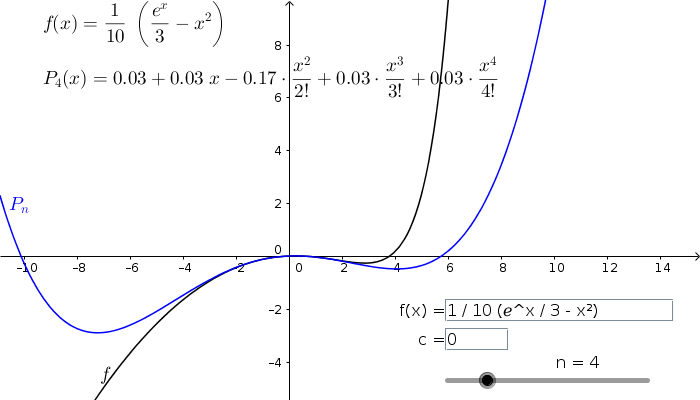
\includegraphics[width=12cm,keepaspectratio=true]{03_Taylorrod.png}
\end{center}



\subsection{Setning}
\label{kafli10:id4}
Taylormargliða með miðju í \(c\) fyrir \(f\) er skilgreind sem
margliðan
\begin{equation*}
\begin{split}\begin{aligned}
  P_n(x)& =\sum_{n=0}^n \frac{f^{(k)}(c)}{n!}(x-c)^n \\
  &=f(c)+f'(c)(x-c)+ \frac{f''(c)}{2}(x-c)^2+\cdots+\frac{f^{(n)}(c)}{n!}(x-c)^n.\end{aligned}\end{split}
\end{equation*}
Skekkjan í \(n\)-ta stigs Taylornálgun er
\(R_n(x)=f(x)-P_n(x)\).

Til er tala \(X\) sem liggur á milli \(c\) og \(x\) þannig
að
\begin{equation*}
\begin{split}R_n(x)=\frac{f^{(n+1)}(X)}{(n+1)!}(x-c)^{n+1}.\end{split}
\end{equation*}

\subsection{Setning}
\label{kafli10:id5}
Gerum ráð fyrir að \(f\) sé fall sem er óendanlega oft diffranlegt í
punktinum \(c\).

Fyrir fast gildi á \(x\) þá er Taylorröðin
\begin{equation*}
\begin{split}\sum_{n=0}^\infty \frac{f^{(n)}(c)}{n!}(x-c)^n\end{split}
\end{equation*}
samleitin með summu \(f(x)\) ef og aðeins ef
\begin{equation*}
\begin{split}\lim_{n\rightarrow\infty}R_n(x)=0.\end{split}
\end{equation*}
\index{Taylorröð!tvíliðuröð}

\subsection{Dæmi: Tvíliðuröðin}
\label{kafli10:daemi-tviliuroin}\label{kafli10:index-7}
Fyrir \(x\) þannig að \(|x|<1\) og rauntölu \(r\) gildir að
\begin{equation*}
\begin{split}\begin{aligned}
(1+x)^r =& 1+rx+\frac{r(r-1)}{2!}x^2+ \frac{r(r-1)(r-2)}{3!}x^3 \\
&+\frac{r(r-1)(r-2)(r-3)}{4!}x^4+\cdots\\
=& 1+ \sum_{n=1}^\infty \frac{r(r-1)(r-2)\cdots(r-n+1)}{n!}x^n.\end{aligned}\end{split}
\end{equation*}

\subsection{Athugasemd}
\label{kafli10:id6}
Ef \(r \in {{\mathbb  N}}\) þá gefur summan að ofan einfaldlega
stuðlanna þegar búið er að margfalda upp úr svigum, og summan er því
endanleg, því þegar \(n \geq r+1\) þá verða stuðlarnir 0.

Ef hins vegar \(r\notin {{\mathbb  N}}\) þá er enginn stuðlanna 0.


\subsection{Taylorraðir nokkra falla}
\label{kafli10:taylorrair-nokkra-falla}\begin{equation*}
\begin{split}\begin{aligned}
e^x&=\sum_{n=0}^\infty\frac{x^n}{n!}
    =1+x+\frac{x^2}{2}+\frac{x^3}{3!}
    +\cdots
  &\mbox{fyrir öll }x\\
\sin x&=  \sum_{n=0}^\infty\frac{(-1)^n}{(2n+1)!}x^{2n+1}
    =x-\frac{x^3}{3!}+\frac{x^5}{5!}-\frac{x^7}{7!}+\cdots
    &\mbox{fyrir öll }x\\
\cos x&=  \sum_{n=0}^\infty\frac{(-1)^n}{(2n)!}x^{2n}
    =1-\frac{x^2}{2!}+\frac{x^4}{4!}-\frac{x^6}{6!}+\cdots
    &\mbox{fyrir öll }x\\
\frac{1}{1-x}&=\sum_{n=0}^\infty x^n
    =1+x+x^2+x^3+\cdots
&\mbox{fyrir }-1<x<1\\
\frac{1}{(1-x)^2}&=\sum_{n=1}^\infty nx^{n-1}
    =1+2x+3x^2+4x^3+\cdots
&\mbox{fyrir }-1<x<1\\
\ln(1+x)&=  \sum_{n=1}^\infty\frac{(-1)^{n-1}}{n}x^n
    =x-\frac{x^2}{2}+\frac{x^3}{3}-\frac{x^4}{4}+\cdots
    &\mbox{fyrir }-1<x\leq 1\\
\tan^{-1} x&=  \sum_{n=0}^\infty\frac{(-1)^n}{2n+1}x^{2n+1}
    =x-\frac{x^3}{3}+\frac{x^5}{5}-\frac{x^7}{7}+\cdots
    &\mbox{fyrir }-1\leq x\leq 1\\\\
\sinh x&=  \sum_{n=0}^\infty\frac{x^{2n+1}}{(2n+1)!}
    =x+\frac{x^3}{3!}+\frac{x^5}{5!}+\frac{x^7}{7!}+\cdots
    &\mbox{fyrir öll } x\\
\cosh x&=  \sum_{n=0}^\infty\frac{x^{2n}}{(2n)!}
    =1+\frac{x^2}{2!}+\frac{x^4}{4!}+\frac{x^6}{6!}+\cdots
    &\mbox{fyrir öll } x\\\end{aligned}\end{split}
\end{equation*}
\emph{I may not have gone where I intended to go, but I think I have ended up where I needed to be.}

-- Douglas Adams, The Long Dark Tea-Time of the Soul


\chapter{Viðauki}
\label{vidauki:viauki}\label{vidauki::doc}
\emph{The story so far:
In the beginning the Universe was created.
This has made a lot of people very angry and been widely regarded as a bad move.}

-- Douglas Adams, The Restaurant at the End of the Universe
\begin{itemize}
%\item {} 
%\DUrole{xref,std,std-ref}{genindex}

\item {} 
  Þessa skrá (pdf) má finna á \\ \url{http://notendur.hi.is/bsm/stae104/Stae104.pdf}
  %Pdf-útgafa af þessum nótum kemur fljótlega

\item{} Rafræna útgáfu af þessum nótum má finna á \\
  \url{http://notendur.hi.is/bsm/stae104/}

\item {} 
GeoGebru skrárnar sem eru notaðar má finna á \\
\url{http://notendur.hi.is/bsm/stae104/Stae104_geogebra.zip}

\item {} 
Námskeiðið á Uglu \\
\url{https://ugla.hi.is/kv/index2.php?sid=219\&namsknr=09101120166}

\item {} 
Námskeiðið á Piazza \\ \url{http://piazza.com/hi.is/fall2016/st104g/home}.

\end{itemize}
\newpage

\bigskip\hrule{}\bigskip



\section{Kennsluáætlun}
\label{vidauki:kennsluaaetlun}
\emph{Reality is frequently inaccurate.}

-- Douglas Adams, The Restaurant at the End of the Universe

\begin{longtable}{c|l|l|l}
\hline
Dags.&
Efni&
Nótur&
Adams Calculus\\
\hline


22.08.16&
1.~Tölur~og~föll&
1.1-1.4&
P.1,~P.2,~P.4,P.5,~P.6,~P.7~\\
24.08.16&
2.~Markgildi~og~samfelldni&
2.1-2.3&
1.2,~1.5~\\
\hline
29.08.16&
3. Markgildi~og~samfelldni&
2.4-2.6&
1.3\\
31.08.16&
3. Markgildi~og~samfelldni&
2.7-2.8&
1.4\\
\hline

05.09.16&
3.~Afleiður&
3.1-3.3&
2.1,~2.2,~2.3\\
07.09.16&
3.~Afleiður&
3.4-3.6&
2.4,~2.5,~2.6
\\
\hline

12.09.16&
3.~Afleiður&
3.7-3.10&
2.8,~2.9,~3.1\\
14.09.16&
3.~Afleiður&
3.11-3.13&
2.7,~4.3,~4.9,~4.10
\\
\hline
19.09.16&
4.~Torræð~föll&
4.1-4.4&
3.2,~3.3,~3.4\\
21.09.16&
4.~Torræð~föll&
4.5-4.7&
3.5,~3.6\\
\hline
26.09.16&
5.~Könnun~falla&
5.1-5.3&
4.5~\\
28.09.16&
5.~Könnun~falla&
5.4-5.6&
4.4,~4.6~\\
\hline
03.10.16&
5.~Könnun~falla&
5.7-5.8&
4.6,~4.8
\\
-&
\textbf{Próf~úr~lesnu~efni}&
-&
-\\
05.10.16&
6.Heildun&
6.1-6.3&
5.1,~5.2,~5.3,~5.4
\\
\hline
10.10.16&
6.~Heildun&
6.4-6.5&
5.5,~2.10\\
12.10.16&
6.~Heildun&
6.6&
5.6,~6.1,~6.2,~6.3,~6.4
\\
\hline

17.10.16&
6.~Heildun&
6.7&
6.5~\\
19.10.16&
7.~Rúmmál,~massi~og~massamiðjur&
7.1&
7.1,~7.2,~7.3\\

\hline

24.10.16&
7.~Rúmmál,~massi~og~massamiðjur&
7.2-7.3&
7.4,~7.5\\
26.10.16&
8.~Diffurjöfnur&
8.1-8.2&
7.9,~18.1,~18.2\\

\hline

31.10.16&
8.~Diffurjöfnur&
8.3-8.5&
3.7,~18.4,~18.5\\
02.11.16&
Hagnýtingar&
ítarefni&
-\\
-&
\textbf{Próf~úr~heimadæmum}&
-&
-\\

\hline

07.11.16&
9.~Runur~og~raðir&
9.1-9.2&
9.1,~9.2\\
09.11.16&
9.~Runur~og~raðir&
9.3-9.4&
9.2,~9.3\\

\hline

14.11.16&
10.~Veldaraðir&
10.1&
9.3,~9.5\\
16.11.16&
10.~Veldaraðir&
10.2&
9.5\\

\hline

21.11.16&
10.~Veldaraðir&
10.3&
9.6\\
23.11.16&
Samantekt~og~prófundirbúningur&
gamalt~próf&
\\
\hline
\end{longtable}


Kaflanúmer í Adam’s Calculus miðast við 8. útgáfu kennslubókarinnar.


\bigskip\hrule{}\bigskip

\newpage
 
\section{Skipulag námskeiðsins}
\label{vidauki:skipulag-namskeisins}
\emph{You know,'' said Arthur, ``it's at times like this, when I'm trapped in a
Vogon airlock with a man from Betelgeuse, and about to die of asphyxiation
in deep space that I really wish I'd listened to what my mother told me when I was young.''}

\emph{``Why, what did she tell you?''}

\emph{``I don't know, I didn't listen.”}

-- Douglas Adams, The Hitchhiker's Guide to the Galaxy

\textbf{Námsefni:} Viðfangsefni námskeiðsins er stærðfræðigreining í einni
breytistærð; markgildi, samfelldni, diffrun, heildun, diffurjöfnur,
runar og raðir, ásamt hagnýtingum á þessum hlutum.

\textbf{Kennslubók:} Kennslubókin er \emph{Calculus: A Complete Course}, eftir
Robert Adams, 8. útgáfa. Við munum fara í gegnum kafla 1-7, 9 og
18. Einnig er hægt að nota 7. eða 6. útgáfu, þær eru að mestu leyti eins og sú 8.

\textbf{Fyrirlestrar:} Fyrirlestrar eru á mánudögum 8:20-9:50 og á
10:00-11:30 miðvikudögum.

\textbf{Dæmablöð og dæmatímar:} Fyrir hverja viku er gefið út dæmablað sem
verður sett í \emph{Verkefna} möppuna á Uglunni. Á dæmablaðinu eru sett fyrir
skiladæmi og dæmi fyrir dæmatíma.

\textbf{Skiladæmi:} Í hverri viku, nema þegar próf eru, þá eru sett fyrir
skiladæmi. Skiladæmunum á að skila fyrir 16:00 á fimmtudögum í hólf
dæmatímakennara, en þau eru staðsett í andyri VRII. Lausnirnar eiga að
vera snyrtilega uppsettar, ekki í möppu og merktar nafni ykkar og
dæmatímakennara á \textbf{fremstu síðu}. Ég mun setja lausnir við
skiladæmunum í möppuna \emph{Lausnir} á Uglunni.

Frekari leiðbeiningar um frágang og framsetningu skiladæma er að finna
hér fyrir neðan.

\begin{center}\textbf{Til að öðlast próftökurétt þarf að skila
að minnsta kosti 7 af 10 heimadæmum.}
\end{center}
Undanþágur frá þessari reglu fást eingöngu fyrir atbeina Náms- og starfsráðgjafar Háskólans.

Heimadæmin eru einstaklingsverkefni og ef tveir eða fleiri nemendur skila
eins verkefnum þá verða skil ekki gefin skil fyrir.

\textbf{Námsmat:} Á misserinu verða tvö stutt próf, annað úr lesnu efni og
hitt úr skiladæmum. Þessi próf gilda hvort um sig 15\% af lokaeinkunn, en
þó eingöngu til hækkunar. Fyrra prófið verður 3. október og verður þá
spurt úr lesnu efni; skilgreiningum, setningum og sönnunum. Seinna
prófið er 2. nóvember og verður þá spurt um dæmi og atriði sem hafa
komið fyrir á skiladæmunum.

Svindl á prófunum verður
tilkynnt deildarforseta og sett í
farveg innan sviðsins (sbr.
\href{http://www.hi.is/adalvefur/reglur\_fyrir\_haskola\_islands\#51}{51. gr. rgl. 569/2009 HÍ} (http://www.hi.is/adalvefur/reglur\_fyrir\_haskola\_islands\#51)).

Lokaprófið er þriggja tíma skriflegt próf og gildir það 70\% á móti
misserisprófunum tveimur. Nauðsynlegt og nægjanlegt er að fá 5 á
lokaprófinu til þess að standast námskeiðið. Engin hjálpargögn eru
leyfileg í prófinu, en með því fylgir formúlublað.
Vasareiknar eru ekki leyfðir í prófinu.

\textbf{Viðtalstímar:} Ég er með skrifstofu á þriðju hæð í Tæknigarði,
herbergi 325, og verð með viðtalstíma á milli 10:00 og 12:00 á
mánudögum. Ef þið viljið finna mig utan þess tíma væri gott að þið
hefðuð samband fyrst með tölvupósti, netfangið mitt er \href{mailto:bsm@hi.is}{bsm@hi.is}. Einnig
má senda fyrirspurnir í tölvupósti.


\bigskip\hrule{}\bigskip

\newpage

\section{Frágangur skiladæma}
\label{vidauki:fragangur-skiladaema}
\emph{A learning experience is one of those things that says,
`You know that thing you just did? Don't do that.}

-- Douglas Adams, The Salmon of Doubt
\begin{itemize}
\item {} 
Skrifið upp \textbf{dæmið} og lausnina snyrtilega

\item {} 
Vísið í setningar sem þið notið

\item {} 
Notið ekki rökfræðitákn eins og \(\Leftarrow\),
\(\Rightarrow\), \(\Leftrightarrow\), \(\wedge\),
\(\vee\)

\item {} 
Textinn á að vera samfelldur og læsilegur (lesið hann sjálf yfir)

\item {} 
Skýrt svar/niðurstaða

\emph{“Forty-two!” yelled Loonquawl. “Is that all you’ve got to show for
seven and a half million years’ work?”}

\emph{“I checked it very thoroughly,” said the computer, “and that quite
definitely is the answer. I think the problem, to be quite honest with
you, is that you’ve never actually known what the question is.”}

-Douglas Adams, The Hitchhiker's Guide to the Galaxy

\end{itemize}


\bigskip\hrule{}\bigskip

\newpage

\section{Ítarefni}
\label{vidauki:itarefni}
\emph{I refuse to answer that question on the grounds that I don't know the answer.}

-- Douglas Adams

Fyrir nánari útlistun á hugtökunum sem við fjöllum um þá er hægt að skoða,
auk kennslubókarinnar,
\begin{itemize}
\item {} 
\href{http://stae.is}{http://stæ.is} (http://stae.is) (hugtakasafn og orðaskrá)

\item {} 
\url{http://planetmath.org}

\item {} 
\url{http://mathworld.wolfram.com}

\item {} 
\url{http://en.wikipedia.org} (ath. enska útgáfan)

\item {} 
\url{http://tutor-web.net/math}

\end{itemize}


\subsection{Forrit}
\label{vidauki:forrit}\begin{itemize}
\item {} 
GeoGebra \url{http://www.geogebra.org}

\item {} 
WolframAlpha \url{http://www.wolframalpha.com}

\item {} 
Matlab \url{http://www.mathworks.com}
(sjá \url{https://notendur.hi.is/~jonasson/matlab/})

\item {} 
Octave \url{http://www.gnu.org/software/octave/} (opið og ókeypis, svipað og Matlab)

\item {} 
Sage \url{http://www.sagemath.org/}  (opið og ókeypis, byggt á Python)

\item {} 
Mathematica \url{http://www.wolfram.com/mathematica/}

\end{itemize}
\newpage

\bigskip\hrule{}\bigskip



\section{Að læra stærðfræði}
\label{vidauki:a-laera-staerfraei}
\emph{Eftir Rögnvald G. Möller}


\subsection{Að lesa}
\label{vidauki:a-lesa}
Í fyrirlestrum gefst aðeins
tími til að fara yfir helstu atriði námsefnisins og verðið þið að
að kynna ykkur stóran hluta þess upp á eigin spýtur. Sumir nemendur
hafa farið í gegnum framhaldsskóla með því
læra utan að reikniaðferðir og vart reynt að skilja námsefnið.  Hættan
við þessa námsaðferð er að allt fari
í einn graut, og
nemendur geti ekki yfirfært þekkingu sína á önnur svipuð verkefni.
Því held ég að léttasta leiðin í gegnum stærðfræðinámskeiðin í námi
ykkar sé að skilja efnið.  Skilningur á efninu fæst með því að rýna í
skilgreiningar og reglur, skoða sannanir og tengja við dæmi.
Þið \{bf verðið\} að lesa
kennslubókina og kynna ykkur efni fyrirlestra.
Stór hluti þess sem þið munuð fást við í
háskólanámi ykkar er aðeins skiljanlegur þegar notað er tungumál
stærðfræðinnar.  Ef þið leggið það á ykkur að verða læs á tungumál
stærðfræðinnar þá munið þið njóta þess í öllu ykkar námi.


\subsection{Að reikna}
\label{vidauki:a-reikna}
Dæmaskammtarnir eru stórir.  Mörg dæmanna eru hugsuð
sem léttar reikniæfingar.
Önnur dæmi eru til að æfa
meðferð hugtaka og að hjálpa ykkur að skilja
skilgreiningarnar.  Það er ekki nóg að læra niðurstöður, reglur og
reikniaðferðir: til að geta beitt þeim af öryggi þarf að hafa góðan
skilning á þeim grundvallarhugtökunum.

Til að hafa fullt gagn af dæmatímunum þurfið þið að reyna við dæmin
áður en þið mætið í dæmatímann.
Ég hvet ykkur eindregið til að vinna saman í náminu.  Þannig getur
maður fengið hjálp þegar maður er strand og
einnig skerpir fátt skilning manns  jafn mikið og að útskýra
fyrir öðrum.  Námið verður  skemmtilegra og þannig
léttara.


\subsection{Einbeiting}
\label{vidauki:einbeiting}
Meiri árangur næst í náminu ef þið eruð einbeitt.
Það er hægt að blekkja sjálfan sig í að halda að maður hafi verið að
læra allan daginn þegar í raun var deginum eitt í spjall við félagana,
netvafr, fésbókar stúss, msn, tölvuleiki, hlusta á ipodinn, og
svo framvegis.


\subsection{Frágangur skiladæma}
\label{vidauki:id1}
Leggið áherslu á vandaða og agaða framsetningu á lausnum
skiladæmanna.  Það að setja lausnina skýrt og skipulega fram er
nauðsynlegt til að maður sjálfur skilji lausnina til hlítar.

Líkt og venjulegt tal- og ritmál þá hefur mál stærðfræðinnar sína
málfræði, t.d. krefst táknið ``\(=\)'' þess að sitthvoru megin við
það standi stærðir eða stærðtákn, og ef fullyrðing sem er sett fram er
rétt þá eru þessar stærðir jafnar. Sitthvoru megin við táknið
``\(\Rightarrow\)'' varða að standa fullyrðingar, og þegar það er
notað rétt þá er fullyrðing hægra megin afleiðing fullyrðingarinnar
vinstra megin, þ.e.a.s. alltaf þegar fullyrðing vinstra megin er sönn þá
er fullyrðingin hægrra megin líka sönn.

Táknin ``\(\Rightarrow\)'', ``\(\Leftrightarrow\)'' eru hentug
þegar útreikningar eru sýndir á töflu, en mín ráðlegging er að nota þau
sem minnst. Þau eru ekki notuð í kennslubókinni, ekki heldur í
lausnaheftinu, og atvinnustærðfræðingar nota þessi tákn ekki í sínum
skrifum. Í löngum útreikngum er oft hægt að nota ``\(=\)'' í stað
leiðingaörva. Engin ástæða er heldur til að nota táknin
``\(\vee\)'', ``\(\wedge\)'' því orðin ``eða'' og ``og'' eru mun
skýrari; það eina sem táknin hafa fram yfir orðin er tilgerðin.

Gott er að hafa eftirfarandi reglur í huga þegar gengið er frá lausnum
verkefna:
\begin{enumerate}
\item {} 
Textinn á að vera ein samfelld heild sem fullnægir sömu kröfum og
gerðar eru til annars ritaðs máls. Stærðfræðiformúla eða stærðtákn á
aldrei að koma fyrir eitt sér, heldur alltaf að vera felt inn í samfellt
mál.

\item {} 
Uppsetningin á að vera aðlaðandi og frágangur snyrtilegur.

\item {} 
Allar fullyrðingar skulu studdar ljósum rökum.

\item {} 
Svara þarf því sem spurt er um! Það þarf að koma skýrt fram hvert
svarið er.

\end{enumerate}




\chapter{Orðaskrá}
\label{ordaskra:oraskra}\label{ordaskra::doc}
\emph{andhverfanlegur} : invertible

\emph{andhverfur breiðbogakósínus} : inverse hyperbolic cosine


\emph{andhverfur breiðbogasínus} : area-hyperbolic sine

\emph{andhverfur breiðbogatangens} : inverse hyperbolic tangent


\emph{bakmengi} : codomain

\emph{bil} : interval


\emph{breiðbogakósínus} : hyperbolic cosine


\emph{breiðbogasínus} : hyperbolic sine


\emph{breiðbogatangens} : hyperbolic tangent


\emph{diffranlegur} : differentiable


\emph{diffurjafna} : differential equation


\emph{efra mark} : least upper bound

\emph{eintækur} : injective

\emph{fall} : function


\emph{gagntækur} : bijective

\emph{gildi} : image

\emph{heilda} : integrate


\emph{heildanlegur} : integrable


\emph{heildismark} : limit of integration


\emph{heiltala} : integer

\emph{hliðruð línuleg diffurjafna} : inhomogeneous linear differential equation

\emph{hlutheildun} : integration by parts

\emph{hvelft fall} : concave function


\emph{hverfipunktur} : flex point

\emph{innri punktur} : inner point

\emph{innsetning} : change of variables

\emph{jafnstæður} : even


\emph{jaðarpunktur} : boundary point

\emph{keila} : cone


\emph{kennijafna} : characteristic equation


\emph{kúpt fall} : convex function


\emph{línuleg diffurjafna} : linear differential equation


\emph{meðalgildi} : average value

\emph{meðalgildissetning} : mean value theorem


\emph{miðja} : centre

\emph{myndmengi} : actual range

\emph{náttúrleg tala} : natural number


\emph{náttúrlegur logri} : natural logarithm


\emph{rauntala} : real number


\emph{ræð tala} : rational number


\emph{rótarpróf} : root test


\emph{röð} : infinite series

\emph{samfelldni} : continuity


\emph{samfellt fall} : continuous function


\emph{samleitin röð} : convergent series


\emph{samleitnibil} : interval of convergence


\emph{samleitnigeisli} : radius of convergence


\emph{samsemdarvörpun} : identity mapping


\emph{samskeyting} : composite


\emph{skilgreiningarmengi} : argument domain

\emph{snertill} : tangent line

\emph{staðbundið hágildi} : local maximum

\emph{staðbundið lággildi} : local minimum

\emph{staðbundið útgildi} : extremum in the small

\emph{stofnbrotaliðun} : expansion in partial fractions

\emph{stofnfall} : antiderivative

\emph{tvinntala} : complex number


\emph{tölugildi} : absolute value

\emph{undirsumma} : lower sum


\emph{veldaröð} : power series


\emph{veldisvísisfall} : exponential function


\emph{vægi} : moment

\emph{vörpun} : mapping

\emph{yfirsumma} : upper sum


\emph{átækur} : onto

\emph{óeiginlegt heildi} : improper integral


\emph{óræð tala} : irrational number


\chapter{Atriðaskrá}
\printindex
\end{document}
